%%%%%%%%%%%%%%%%%%%%%%%%%%%%%%%%%%%%%%%%%%%%%%%%%%%%%%%%%%%%%%%%%%%%%%%%%%%%%%%%
%% Plantilla de memoria en LaTeX para la EIF - Universidad Rey Juan Carlos
%%
%% Por Gregorio Robles <grex arroba gsyc.urjc.es>
%%     Grupo de Sistemas y Comunicaciones
%%     Escuela de Ingeniería de Fuenlabrada
%%     Universidad Rey Juan Carlos
%% (muchas ideas tomadas de Internet, colegas del GSyC, antiguos alumnos...
%%  etc. Muchas gracias a todos)
%%
%% La última versión de esta plantilla está siempre disponible en:
%%     https://github.com/gregoriorobles/plantilla-memoria
%%
%% Para obtener PDF, ejecuta en la shell:
%%   make
%% (las imágenes deben ir en PNG o JPG)

%%%%%%%%%%%%%%%%%%%%%%%%%%%%%%%%%%%%%%%%%%%%%%%%%%%%%%%%%%%%%%%%%%%%%%%%%%%%%%%%

\documentclass[a4paper, 12pt]{book}
%\usepackage[T1]{fontenc}

\usepackage[a4paper, left=2.5cm, right=2.5cm, top=3cm, bottom=3cm]{geometry}
\usepackage{times}
\usepackage[utf8]{inputenc}
\usepackage[spanish]{babel} % Comenta esta línea si tu memoria es en inglés
\usepackage{url}
%\usepackage[dvipdfm]{graphicx}
\usepackage{graphicx}
\usepackage{float}  %% H para posicionar figuras
\usepackage[nottoc, notlot, notlof, notindex]{tocbibind} %% Opciones de índice
\usepackage{latexsym}  %% Logo LaTeX
\usepackage{booktabs}
% Escribe el título y el nombre del autor / autora para que se use bien
% en otras partes de la plantilla
% Dependiendo de las partes de la plantilla, a veces aparecerán tal
% cual los escribas, a veces totalmente en mayúsculas, a veces de otras
% formas
\title{ANÁLISIS DEL USO DE LENGUAJES DE PROGRAMACIÓN MINORITARIOS EN PROYECTOS DE SOFTWARE LIBRE}
\author{Raúl Gómez Cantador}

% Guarda el título, el autor y la fecha en variables
\makeatletter
\let\thetitle\@title
\let\theauthor\@author
\let\thedate\@date
\makeatother

\renewcommand{\baselinestretch}{1.5}  %% Interlineado

\begin{document}

\renewcommand{\refname}{Bibliografía}  %% Renombrando
\renewcommand{\appendixname}{Apéndice}


%%%%%%%%%%%%%%%%%%%%%%%%%%%%%%%%%%%%%%%%%%%%%%%%%%%%%%%%%%%%%%%%%%%%%%%%%%%%%%%%
% PORTADA

\begin{titlepage}
  \begin{center}
    \includegraphics[scale=0.6]{img/URJ_logo_Color_POS.png}

    \vspace{1.75cm}

    \LARGE
    ESCUELA DE INGENIERÍA DE FUENLABRADA
    \vspace{1cm}

    \LARGE
    GRADO EN INGENIERÍA EN SISTEMAS AUDIOVISUALES Y MULTIMEDIA

    \vspace{1cm}
    \LARGE
    \textbf{TRABAJO FIN DE GRADO}

    \vspace{2cm}

    \Large
    \MakeUppercase{\thetitle}

    \vspace{2cm}

    \large
    Autor : \theauthor \\
    Tutor : Dr. Gregorio Robles Martínez\\
    \vspace{1cm}

    \large
    Curso académico 2024/2025

  \end{center}
\end{titlepage}

\newpage
\mbox{}
\thispagestyle{empty} % para que no se numere esta pagina



%%%%%%%%%%%%%%%%%%%%%%%%%%%%%%%%%%%%%%%%%%%%%%%%%%%%%%%%%%%%%%%%%%%%%%%%%%%%%%%%
%%%% Para firmar
\clearpage
\pagenumbering{gobble}
\chapter*{}

\vspace{-4cm}
\begin{center}
  \LARGE
  \textbf{Trabajo Fin de Grado/Máster}

  \vspace{1cm}
  \large
  \thetitle

  \vspace{0.8cm}
  \large
  \textbf{Autor :} \theauthor \\
  \textbf{Tutor :} Dr. Gregorio Robles Martínez

\end{center}

\vspace{0.8cm}
La defensa del presente Proyecto Fin de Carrera se realizó el día \qquad$\;\,$ de diciembre \newline de 2024, siendo calificada por el siguiente tribunal:


\vspace{0.5cm}
\textbf{Presidente:}

\vspace{1cm}
\textbf{Secretario:}

\vspace{1cm}
\textbf{Vocal:}


\vspace{1cm}
y habiendo obtenido la siguiente \textbf{Calificación:}


\vspace{1cm}
\begin{flushright}
  Fuenlabrada, a \qquad$\;\,$ de diciembre de 2024
\end{flushright}

\vspace{1cm}

%% Licencia de publicación en abierto elegida
%% Ver detalles en https://ofilibre.urjc.es/guias/tfg-abierto/
\includegraphics[scale=0.6]{img/by-sa}
%\includegraphics[scale=0.6]{img/by}

%% Poner el año adecuado
\noindent©2024 \theauthor  \\
Algunos derechos reservados  \\
Este documento se distribuye bajo la licencia ``Atribución-CompartirIgual 4.0 Internacional'' de Creative Commons, disponible en \\
\url{https://creativecommons.org/licenses/by-sa/4.0/deed.es}


%%%%%%%%%%%%%%%%%%%%%%%%%%%%%%%%%%%%%%%%%%%%%%%%%%%%%%%%%%%%%%%%%%%%%%%%%%%%%%%%
%%%% Dedicatoria

\chapter*{}
\pagenumbering{Roman} % para comenzar la numeracion de paginas en numeros romanos
\begin{flushright}
  \textit{Dedicado a \\
    mi familia.}
\end{flushright}

%%%%%%%%%%%%%%%%%%%%%%%%%%%%%%%%%%%%%%%%%%%%%%%%%%%%%%%%%%%%%%%%%%%%%%%%%%%%%%%%
%%%% Agradecimientos

\chapter*{Agradecimientos}
%\addcontentsline{toc}{chapter}{Agradecimientos} % si queremos que aparezca en el índice
\markboth{AGRADECIMIENTOS}{AGRADECIMIENTOS} % encabezado 

Con este proyecto doy prácticamente el carpetazo final a mi paso por la universidad. Han sido seis años que por algunas épocas se han hecho muy cuesta arriba.  Sin embargo, me quedo con todos aquellos momentos buenos que he pasado, que son infinitamente mayores que los malos. Quiero agradecer a todas las personas que me han ayudado a lo largo de todo este proceso y en especial a los amigos que he hecho durante el camino.

También, quiero agradecer a Gregorio, mi tutor, por ser tan flexible conmigo. Aunque por mi parte no haya sido muy organizado durante la realización del proyecto y me haya faltado constancia, siempre que he recurrido a ti para hacer cualquier tutoría, has sacado algún tiempo para ayudarme, incluso siendo algunas de ellas bastante tarde. ¡Muchas gracias, Gregorio!

Por último, quiero agradecer sobre todo, a mi familia. Siempre que los necesito están ahí y me apoyan en todo lo que hago. Gracias por decirme aquello que necesito oír, y no lo que quiero, siempre.

%%%%%%%%%%%%%%%%%%%%%%%%%%%%%%%%%%%%%%%%%%%%%%%%%%%%%%%%%%%%%%%%%%%%%%%%%%%%%%%%
%%%% Resumen

\chapter*{Resumen}
%\addcontentsline{toc}{chapter}{Resumen} % si queremos que aparezca en el índice
\markboth{RESUMEN}{RESUMEN} % encabezado

Este proyecto consiste en la creación de una herramienta que permite realizar el análisis de uso de los lenguajes minoritarios en repositorios públicos de GitHub. Entendemos los lenguajes minoritarios por aquellos que representan un porcentaje pequeño de uso en un repositorio y que es usado por un grupo pequeño de usuarios. El objetivo que tiene es que el usuario que utilice esta herramienta pueda ver cómo es el uso de estos lenguajes minoritarios en el repositorio que escoja, los usuarios que han contribuido y en qué cantidad.

Para ello se ha realizado un programa en Python que se encarga de producir estos análisis recolectando los datos de la participación histórica de los repositorios a través de los commits mediante el uso de la librería Perceval y otros datos como el número de ficheros o las tecnología usadas en los repositorios. Además, para hacer la representación de los análisis se ha realizado también una aplicación web cliente-servidor para que la visualización de estos sea mucho más cómoda y sencilla de usar para un usuario cualquiera. Esta aplicación se ha construido con HTML, CSS y JavaScript con uso de la librería Bootstrap y con la librería Flask para la gestión del servidor. Además se ha creado una base de datos SQLite3 donde se almacenan los datos de los repositorios analizados, la información de uso de todos los lenguajes y la información de todos los usuarios que hayan participado en alguno de los proyectos.

Puede ser un proyecto útil para desarrolladores que quieran conocer cómo funcionan los lenguajes con menor uso en repositorios, sobre todo, dirigido a aquellos repositorios muy grandes y con bastante tiempo detrás, donde es difícil obtener esta información. 

%%%%%%%%%%%%%%%%%%%%%%%%%%%%%%%%%%%%%%%%%%%%%%%%%%%%%%%%%%%%%%%%%%%%%%%%%%%%%%%%
%%%% Resumen en inglés

\chapter*{Summary}
%\addcontentsline{toc}{chapter}{Summary} % si queremos que aparezca en el índice
\markboth{SUMMARY}{SUMMARY} % encabezado

This project consists of the creation of a tool that allows the analysis of the use of minority languages in public repositories on GitHub. We understand minority languages as those that represent a small percentage of use in a repository and that are used by a small group of users. The aim is that the user who uses this tool can see how these minority languages are used in the repository he/she chooses, the users who have contributed and in what quantity.

To do this, a Python program has been created that is responsible for producing these analyses by collecting data on the historical participation of the repositories through commits using the Perceval library and other data such as the total number of files or the technologies used in the repositories. In addition, a client-server web application has also been developed to represent the analyses so the visualisation of these analyses is much more comfortable and easy to use for any user. This application has been built with HTML, CSS and JavaScript using the Bootstrap library and the Flask library for server management. Also, a SQLite3 database has been created where the data of the analysed repositories, the usage information of all the languages and the information of all the users who have participated in any of the projects stored.

It can be a useful project for developers who want to know how the lesser-used languages work in repositories, especially for very large repositories with a long time behind them, where it is difficult to obtain this information. 


%%%%%%%%%%%%%%%%%%%%%%%%%%%%%%%%%%%%%%%%%%%%%%%%%%%%%%%%%%%%%%%%%%%%%%%%%%%%%%%%
%%%%%%%%%%%%%%%%%%%%%%%%%%%%%%%%%%%%%%%%%%%%%%%%%%%%%%%%%%%%%%%%%%%%%%%%%%%%%%%%
% ÍNDICES %
%%%%%%%%%%%%%%%%%%%%%%%%%%%%%%%%%%%%%%%%%%%%%%%%%%%%%%%%%%%%%%%%%%%%%%%%%%%%%%%%

% Las buenas noticias es que los índices se generan automáticamente.
% Lo único que tienes que hacer es elegir cuáles quieren que se generen,
% y comentar/descomentar esa instrucción de LaTeX.

%%%% Índice de contenidos
\tableofcontents
%%%% Índice de figuras
\cleardoublepage
\addcontentsline{toc}{chapter}{Lista de figuras} % para que aparezca en el indice de contenidos
\listoffigures % indice de figuras
%%%% Índice de tablas
%\cleardoublepage
%\addcontentsline{toc}{chapter}{Lista de tablas} % para que aparezca en el indice de contenidos
%\listoftables % indice de tablas


%%%%%%%%%%%%%%%%%%%%%%%%%%%%%%%%%%%%%%%%%%%%%%%%%%%%%%%%%%%%%%%%%%%%%%%%%%%%%%%%
%%%%%%%%%%%%%%%%%%%%%%%%%%%%%%%%%%%%%%%%%%%%%%%%%%%%%%%%%%%%%%%%%%%%%%%%%%%%%%%%
% INTRODUCCIÓN %
%%%%%%%%%%%%%%%%%%%%%%%%%%%%%%%%%%%%%%%%%%%%%%%%%%%%%%%%%%%%%%%%%%%%%%%%%%%%%%%%

\cleardoublepage
\chapter{Introducción}
\label{sec:intro} % etiqueta para poder referenciar luego en el texto con ~\ref{sec:intro}
\pagenumbering{arabic} % para empezar la numeración de página con números

% En este capítulo se introduce el proyecto.
% Debería tener información general sobre el mismo, dando la información sobre el contexto en el que se ha desarrollado.

% No te olvides de echarle un ojo a la página con los cinco errores de escritura más frecuentes\footnote{\url{http://www.tallerdeescritores.com/errores-de-escritura-frecuentes}}.

% Aconsejo a todo el mundo que mire y se inspire en memorias pasadas.
% Las memorias de los proyectos que he llevado yo están (casi) todas almacenadas en mi web del GSyC\footnote{\url{https://gsyc.urjc.es/~grex/pfcs/}}.

% En mayo de 2023 me apunté a un curso de innovación docente donde nos pidieron hacer un podcast con temática docente. Aproveché entonces para hacer un podcast de unos 30 minutos donde en los primeros quince minutos introducía LaTeX y la memoria, y en los segundos hacía hincapién en aquellas cosas que más os cuestan utilizar en la memoria: las figuras, las tablas y las citas. Podéis escuchar el podcast en Internet\footnote{\url{https://podcasters.spotify.com/pod/show/gregorio-robles9/episodes/Tu-memoria-de-Trabajo-Fin-de-Grado-o-de-Mster-en-LaTeX-e23hucr/a-a58kp2}}.

Durante los últimos años, a través de plataformas de desarrollo de software como GitHub o GitLab, una gran cantidad de desarrolladores contribuyen diariamente a proyectos de software libre. Por supuesto, al haber tanta variedad de proyectos y desarrolladores, existe una gran diversidad de lenguajes de programación que se usan en los distintos repositorios de cada uno de los proyectos. Este trabajo de fin de grado tiene como objetivo realizar el análisis del uso de esos lenguajes de programación, dividiéndolos en dos clases: lenguajes mayoritarios y lenguajes minoritarios, si bien, nos centraremos en mayor medida en estos últimos. Definimos estos lenguajes minoritarios como aquellos que representan menos de un 5\% dentro de un repositorio donde se almacene el código de un programa, y que es usado por un número pequeño de contribuyentes. Estos lenguajes, si bien no son los más usados por la gran mayoría de desarrolladores, pueden llegar a cumplir roles específicos y críticos para el funcionamiento de una aplicación o proyecto.

Para llevar a cabo este análisis, se ha desarrollado una aplicación en Python cuyo objetivo es la recopilación y representación de datos provenientes de los repositorios de distintos proyectos para comprobar cómo es el uso de estos lenguajes minoritarios. Con todos estos datos, se ha creado una base de datos SQL que contiene la información de uso de los distintos lenguajes por usuario y repositorio de todos los proyectos que se han analizado a lo largo de la ejecución del trabajo de fin de grado.

Además, este proyecto cuenta con una aplicación web para poder facilitar la recolección y representación de los datos de manera mucho más fácil y cómoda. Esta herramienta se puede utilizar para hacer el análisis del uso de los lenguajes minoritarios dentro de un repositorio para ver como se han gestionado estos a lo largo del tiempo. Además, permite conocer a los usuarios que han participado a los repositorios y con ello, poder hacerse una idea de los conocimientos de cada uno de ellos. Además. puesto que existe una base de datos que va almacenando todos estos análisis, en el futuro podría servir para seguir recopilando datos de repositorios distintos a los que se han usado para realizar este análisis y continuar investigando más adelante. 

\section{Estructura de la memoria}
\label{sec:estructura}

La memoria se estructura de la siguiente manera:


\begin{itemize}
  \item \textbf{Capítulo 1: Introducción.} Se presenta la motivación y una breve descripción de lo que se afronta en este proyecto, además de informar de la estructura del mismo.

  \item \textbf{Capítulo 2: Objetivos.} Se describen los objetivos a alcanzar durante toda la consecución del proyecto, incluyendo tanto planificación temporal como objetivos técnicos.

  \item \textbf{Capítulo 3: Estado del arte.} Explicación de las distintas tecnologías usadas a lo largo del proyecto. Incluye la información sobre la aplicación web, y como se realiza la recopilación y guardado de datos en la base de datos.

  \item \textbf{Capítulo 4: Diseño e implementación.} Se realiza una explicación sobre el diseño en conjunto de todo el proyecto, y el por qué de como se ha implementado.

  \item \textbf{Capítulo 5: Experimentos y validación.} Se explica un caso de uso de la aplicación para ver las funcionalidades y comprobar que son correctas.

  \item \textbf{Capítulo 6: Resultados.} Se realiza el análisis final de los resultados obtenidos tras analizar 200 repositorios.

  \item \textbf{Capítulo 7: Conclusiones.} Incluye la conclusión final del proyecto.

\end{itemize}

%%%%%%%%%%%%%%%%%%%%%%%%%%%%%%%%%%%%%%%%%%%%%%%%%%%%%%%%%%%%%%%%%%%%%%%%%%%%%%%%
%%%%%%%%%%%%%%%%%%%%%%%%%%%%%%%%%%%%%%%%%%%%%%%%%%%%%%%%%%%%%%%%%%%%%%%%%%%%%%%%
% OBJETIVOS %
%%%%%%%%%%%%%%%%%%%%%%%%%%%%%%%%%%%%%%%%%%%%%%%%%%%%%%%%%%%%%%%%%%%%%%%%%%%%%%%%

\cleardoublepage % empezamos en página impar
\chapter{Objetivos} % título del capítulo (se muestra)
\label{chap:objetivos} % identificador del capítulo (no se muestra, es para poder referenciarlo)

\section{Objetivo general} % título de sección (se muestra)
\label{sec:objetivo-general} % identificador de sección (no se muestra, es para poder referenciarla)

% Aquí vendría el objetivo general en una frase:
% Mi trabajo fin de grado consiste en crear de una herramienta de análisis de los comentarios jocosos en repositorios de software libre alojados en la plataforma GitHub.

% Recuerda que los objetivos siempre vienen en infinitivo.

Mi trabajo de fin de grado consiste en obtener datos de los repositorios de proyectos de software libre que se encuentren disponibles en la plataforma de desarrollo software GitHub y analizar en profundidad los desarrolladores implicados en los mismos como los lenguajes de programación utilizados para llevarlos a cabo, principalmente aquellos que son minoritarios, pero de uso común.

\section{Objetivos específicos}
\label{sec:objetivos-especificos}

Se han seguido los siguientes objetivos específicos para llegar a cumplir el objetivo final. Cada objetivo específico cuenta con sus propios puntos:

\begin{itemize}
  \item \textbf{Obtención de datos de los repositorios de plataformas Git}
        \begin{itemize}
  \item Búsqueda de una herramienta para obtener los datos usando Python
  \item Investigación del módulo de python Perceval usado para la obtención de commits realizados en los repositorios
  \item Investigación de llamadas a la API de GitHub para obtener información adicional
  \item Guardado de datos en formato JSON para su posterior tratamiento
\end{itemize}
\item \textbf{Tratamiento de los datos de los repositorios}
\begin{itemize}
\item Organización de los datos obtenidos
\item Parsear ficheros JSON de las llamadas a la API de GitHub para guardar únicamente los datos relevantes para el proyecto:
\begin{itemize}
  \item Commits realizados sobre el repositorio
  \item Usuario que ha participado en cada uno de los commits
  \item Lenguaje de programación usado en cada commit
  \item Total de usuarios que han participado en el repositorio
\end{itemize}
\item Creación de un fichero JSON para almacenar todos los datos resultantes del punto anterior:
\end{itemize}
\item \textbf{Creación de una aplicación web para permitir un uso más fácil del aplicativo}
\begin{itemize}
  \item Uso de Flask para construir la aplicación web
  \item Conectividad con la base de datos creada
  \item Permitir al usuario la obtención de los datos de un repositorio a su elección
  \item Representación de los datos de los repositorios
\end{itemize}
\item \textbf{Creación de una base de datos donde almacenar los análisis de los repositorios}
\begin{itemize}
  \item Almacenar repositorios analizados
  \item Almacenar usuarios contribuyentes a cada repositorio analizado
  \item Almacenar usuarios con todas sus contribuciones a cada uno de los repositorios
  \item Almacenar lenguajes usados en cada repositorio
\end{itemize}
\end{itemize}
\section{Planificación temporal}
\label{sec:planificacion-temporal}

El total de duración del proyecto ha sido de aproximadamente un año. Contacté por primera vez con Gregorio, mi tutor, en octubre del año 2023, con la intención de comenzar con este proyecto, dando inicio desde noviembre y terminándolo a lo largo del anterior curso académico 2023/2024. Sin embargo, no ha sido hasta este presente curso 2024/2025 en el que he podido finalizar el trabajo, sobre todo debido a algunos parones que hice durante algunos meses del curso anterior y a que, principalmente, se ha hecho en mi tiempo libre y durante los fines de semana. En la siguiente figura, se encuentra la planificación general final que ha seguido el proyecto a lo largo de todo este año en un diagrama de Gantt:

\begin{figure}[H]
  \centering
  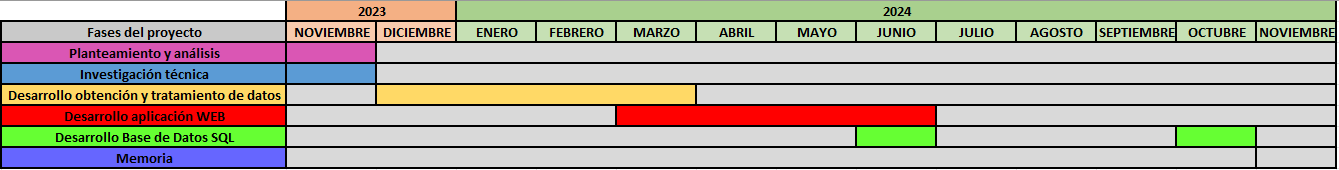
\includegraphics[width=1\textwidth]{img/diagramagantt.png}
  \caption{Diagrama de Gantt de la planificación temporal del proyecto}
    \label{figura:diagrama}
\end{figure}

%%%%%%%%%%%%%%%%%%%%%%%%%%%%%%%%%%%%%%%%%%%%%%%%%%%%%%%%%%%%%%%%%%%%%%%%%%%%%%%%
%%%%%%%%%%%%%%%%%%%%%%%%%%%%%%%%%%%%%%%%%%%%%%%%%%%%%%%%%%%%%%%%%%%%%%%%%%%%%%%%
% ESTADO DEL ARTE %
%%%%%%%%%%%%%%%%%%%%%%%%%%%%%%%%%%%%%%%%%%%%%%%%%%%%%%%%%%%%%%%%%%%%%%%%%%%%%%%%

\cleardoublepage
\chapter{Estado del arte}
\label{chap:estado}

En este proyecto se han utilizado múltiples tecnologías, siendo el lenguaje de programación Python el principal, y en el que se basan prácticamente todos los recursos que he utilizado.

\section{Python}
\label{sec:Python}

Python~\cite{python:_python} es uno de los lenguajes de programación más utilizados durante los últimos años. Se debe, sobre todo, a su accesibilidad y facilidad que ofrece a los desarrolladores para realizar múltiples tareas.

Es un lenguaje de programación de código abierto y gratuito creado por Guido van Rossum a principios de la década de los noventa, pero no ha hecho nada más que evolucionar durante todo este tiempo para agregar nuevas características en cada una de las versiones. Para este trabajo se ha utilizado la versión 3.11 de Python, sin embargo, aún sigue actualizandose, siendo la última versión en el momento de escribir esta memoria la versión 3.13.

Las principales ventajas ~\cite{fernandez:_python} que ofrece sobre otros lenguajes son:

\begin{itemize}
  \item \textbf{Es un lenguaje interpretado}, es decir, no es necesario compilar el código para su ejecución, sino que en su lugar existe un intérprete que se encarga de la lectura del fichero y su ejecución.
  \item \textbf{Es un lenguaje multiplataforma}, por lo que su ejecución no está limitada a un sistema o software específico. Es muy flexible desde este punto de vista.
  \item \textbf{Facilidad de la sintaxis}. Es uno de los lenguajes preferidos para comenzar en el mundo de la programación debido a ello.
  \item \textbf{Existencia de un garbage collector} que permite la limpieza automática de memoria y facilita en gran cantidad evitar gastos de memoria inútiles.
\end{itemize}

En mi caso, lo he escogido en este proyecto ya que, además de ser el lenguaje que más he usado tanto a lo largo de la carrera universitaria como en el mundo laboral, y por tanto ser el lenguaje del que más conocimiento tengo, quería aprender más sobre él usándolo en otros ámbitos que no conocía antes, como la interacción con una base de datos, o la creación de la plataforma web usando el módulo Flask que ofrece el propio Python.

\section{Perceval}
\label{sec:Perceval}
Perceval~\cite{perceval:_perceval} es la librería de Python que me recomendó mi tutor para poder conseguir la mayoría de información necesaria para realizar los análisis de este proyecto. Consiste en un módulo que consigue recuperar datos relacionados con el desarrollo software de varias posibles fuentes como pueden ser Confluence, Bugzilla o Slack, aunque en este trabajo solo se ha usado para obtener datos de repositorios Git.

Del modo que se ha usado Perceval en mi caso, ha sido para poder recuperar los commits de los distintos repositorios en formato JSON, lo que me ha permitido ver el historial de cambios de los repositorios y las personas que han contribuido a los mismos para realizar los análisis.
\section{Flask}
\label{sec:Flask}

Flask~\cite{flask:_flask} es un módulo de Python que consiste en un framework ligero para la creación de aplicaciones web. Está diseñado para ser sencillo y rápido, pero escalable a la construcción de aplicaciones complejas. Se usa en distintos ámbitos como aplicaciones web, como es el caso de este proyecto, pero también en microservicios, desarrollos de APIs...

Se ha escogido Flask sobre otros frameworks para Python como puede ser Django ya que ofrece más flexibilidad y me permitía elegir los demás módulos que fueran necesarios para la personalización de mi web y hacerla de la manera que he pensado.

\section{Jinja2}
\label{sec:Jinja2}

Jinja2~\cite{jinja:_jinja} es el motor de plantillas que usa Flask. Permite la generación de contenido web dinámico en la aplicaciones de manera eficiente y estructurada. Una de sus características principales que se ha usado en este proyecto es la utilización de una estructura base que cualquier otra plantilla puede heredar, lo que permite ahorrar bastante tiempo de desarrollo HTML o CSS.

Su uso me ha permitido crear las páginas dinámicas en la que aparecen los análisis realizados de los repositorios, permitiéndome representarlos de manera sencilla y cómoda para mí como desarrollador, pero también, a imagen del usuario que podría visitar la web, fácil de entender.

\section{Git}
\label{sec:Git}

Git~\cite{git:_git}  es un sistema de control de versiones usado en proyectos de desarrollo de software. Realiza un seguimiento de los cambios en archivos de un proyecto, por lo que es muy útil en los casos donde un grupo de personas realizan estos cambios en los mismos ficheros al mismo tiempo.

Permite a los desarrolladores conocer todo el historial de modificaciones que se han realizado sobre el proyecto, lo que facilita la organización y el alineamiento entre los propios contribuyentes. Se utiliza tanto en proyectos de código abierto y gratuito como este, como en proyectos comerciales de empresas, que utilizan Git para la gestión de versiones del software que crean.


En este proyecto, además de para los repositorios Git que he escogido para realizar el análisis, se ha utilizado para hacer también, el control de versiones de mi propio proyecto, por lo que es fácil ver el progreso que ha seguido mi software a lo largo del tiempo, pues es posible ver el historial de cambios hechos durante este año.

\section{GitHub}
\label{sec:GitHub}

GitHub~\cite{github:_github}  es una plataforma para almacenar, compartir y trabajar junto a otros usuarios en proyectos de desarrollo. Sus principales características son:

\begin{itemize}
  \item Compartir el trabajo junto a otras personas.
  \item Seguir los cambios en el código a lo largo del tiempo, para el control de versiones de un proyecto.
  \item Colaborar en proyectos con multitud de personas.
  \item Permitir a otros usuarios de la plataforma que puedan revisar el código y realizar sugerencias para su mejora.
  \item Creación y gestión de repositorios donde almacenar todo el código de un proyecto.
\end{itemize}

Todos los repositorios analizados en este proyecto forman parte de la propia plataforma de GitHub, incluyendo también mi propio trabajo de fin de grado.

\section{SQLAlchemy}
\label{sec:SQLAlchemy}

SQLAlchemy~\cite{myerscopeland:_essentialsqlalchemy} es una librería de Python usada para la interacción con una gran variedad de bases de datos. Permite crear modelos de datos y consultas de una manera sencilla y cercana a las clases de Python.

Es un ORM (Object Relational Mapper), por lo que permite el mapeo de tablas de las bases de datos sin tener que escribir las consultas, sino que mediante los objetos de Python, podemos hacer esta función.

Lo he usado en mi implementación con la base de datos SQLite que se ha hecho y que contiene el análisis de todos los repositorios.

\section{SQLite}
\label{sec:SQLite}

SQLite~\cite{sqlite:_sqlite} es una base de datos integrada de código abierto. Su principal característica y diferencia con la mayoría de bases de datos SQL es que no tiene un proceso independiente al de la aplicación, sino que se encuentra contenida en la propia aplicación.

Lo he usado por la facilidad que ofrece para la configuración de la propia base de datos, ya que, al estar dentro de la propia aplicación, no necesita configuración de red, lo que facilita bastante el uso de bases de datos para personas como yo, que no son expertos en ello.

\section{HTML}
\label{sec:HTML}

HTML es un lenguaje de marcado que utiliza una serie de etiquetas con el objetivo de dar estructura a un contenido web. Representa el estándar de la visualización de páginas web y es utilizado por todos los grandes navegadores actuales.

Todas las páginas que forman la aplicación web se han creado y estructurado mediante ficheros HTML.

\section{CSS}
\label{sec:CSS}

CSS es el lenguaje mayoritariamente utilizado para dar estilo a una página web. Este lenguaje permite vincular los documentos de texto en formato HTML con hojas de estilo que contiene la información topográfica de los elementos visuales de la página, y que además, permite separar completamente la estructura de los contenidos, del estilo que estos van a tener ya en la visualización en la web.

En este proyecto se ha utilizado CSS en todas las páginas para dar el estilo visual a los contenidos, utilizando además la librería Bootstrap para facilitar un diseño simple y que sirviera de plantilla para tener consistencia visual en toda la aplicación.

\section{Bootstrap}
\label{sec:Bootstrap}

Bootstrap~\cite{bootstrap:_bootstrap} es un proyecto de código abierto que consiste en un framework de front-end que facilita el desarrollo de aplicaciones mediante un conjunto de herramientas y componentes pre-hechos como botones o formularios que permiten la personalización del diseño de una web.

Se ha usado Bootstrap en el diseño de todas las páginas incluyendo botones, formularios, o el encabezado de la página web.


%%%%%%%%%%%%%%%%%%%%%%%%%%%%%%%%%%%%%%%%%%%%%%%%%%%%%%%%%%%%%%%%%%%%%%%%%%%%%%%%
%%%%%%%%%%%%%%%%%%%%%%%%%%%%%%%%%%%%%%%%%%%%%%%%%%%%%%%%%%%%%%%%%%%%%%%%%%%%%%%%
% DISEÑO E IMPLEMENTACIÓN %
%%%%%%%%%%%%%%%%%%%%%%%%%%%%%%%%%%%%%%%%%%%%%%%%%%%%%%%%%%%%%%%%%%%%%%%%%%%%%%%%

\cleardoublepage
\chapter{Diseño e implementación}
\label{sec:diseno}

En este apartado de la memoria se detalla el diseño de la aplicación y de todos sus componentes.

\section{Arquitectura general}
\label{sec:arquitectura}

Este proyecto sigue un modelo cliente-servidor. El cliente en este caso, para el uso que está pensado, sería la aplicación web que se ejecuta desde el navegador y que permite realizar las peticiones de una manera más cómoda, accesible y sencilla al servidor, aunque obviamente, se podrían hacer estas peticiones a mano sin utilizar la aplicación web, y seguiría siendo el cliente. El servidor, mientras tanto, espera a atender las peticiones que se envían a los endpoints que tiene definidos para finalmente dar la respuesta a los clientes.


Aunque en puntos posteriores entraremos más a fondo en cada uno de elementos de la aplicación, el flujo que sigue, a modo general es el siguiente:

\begin{figure}[H]
  \centering
  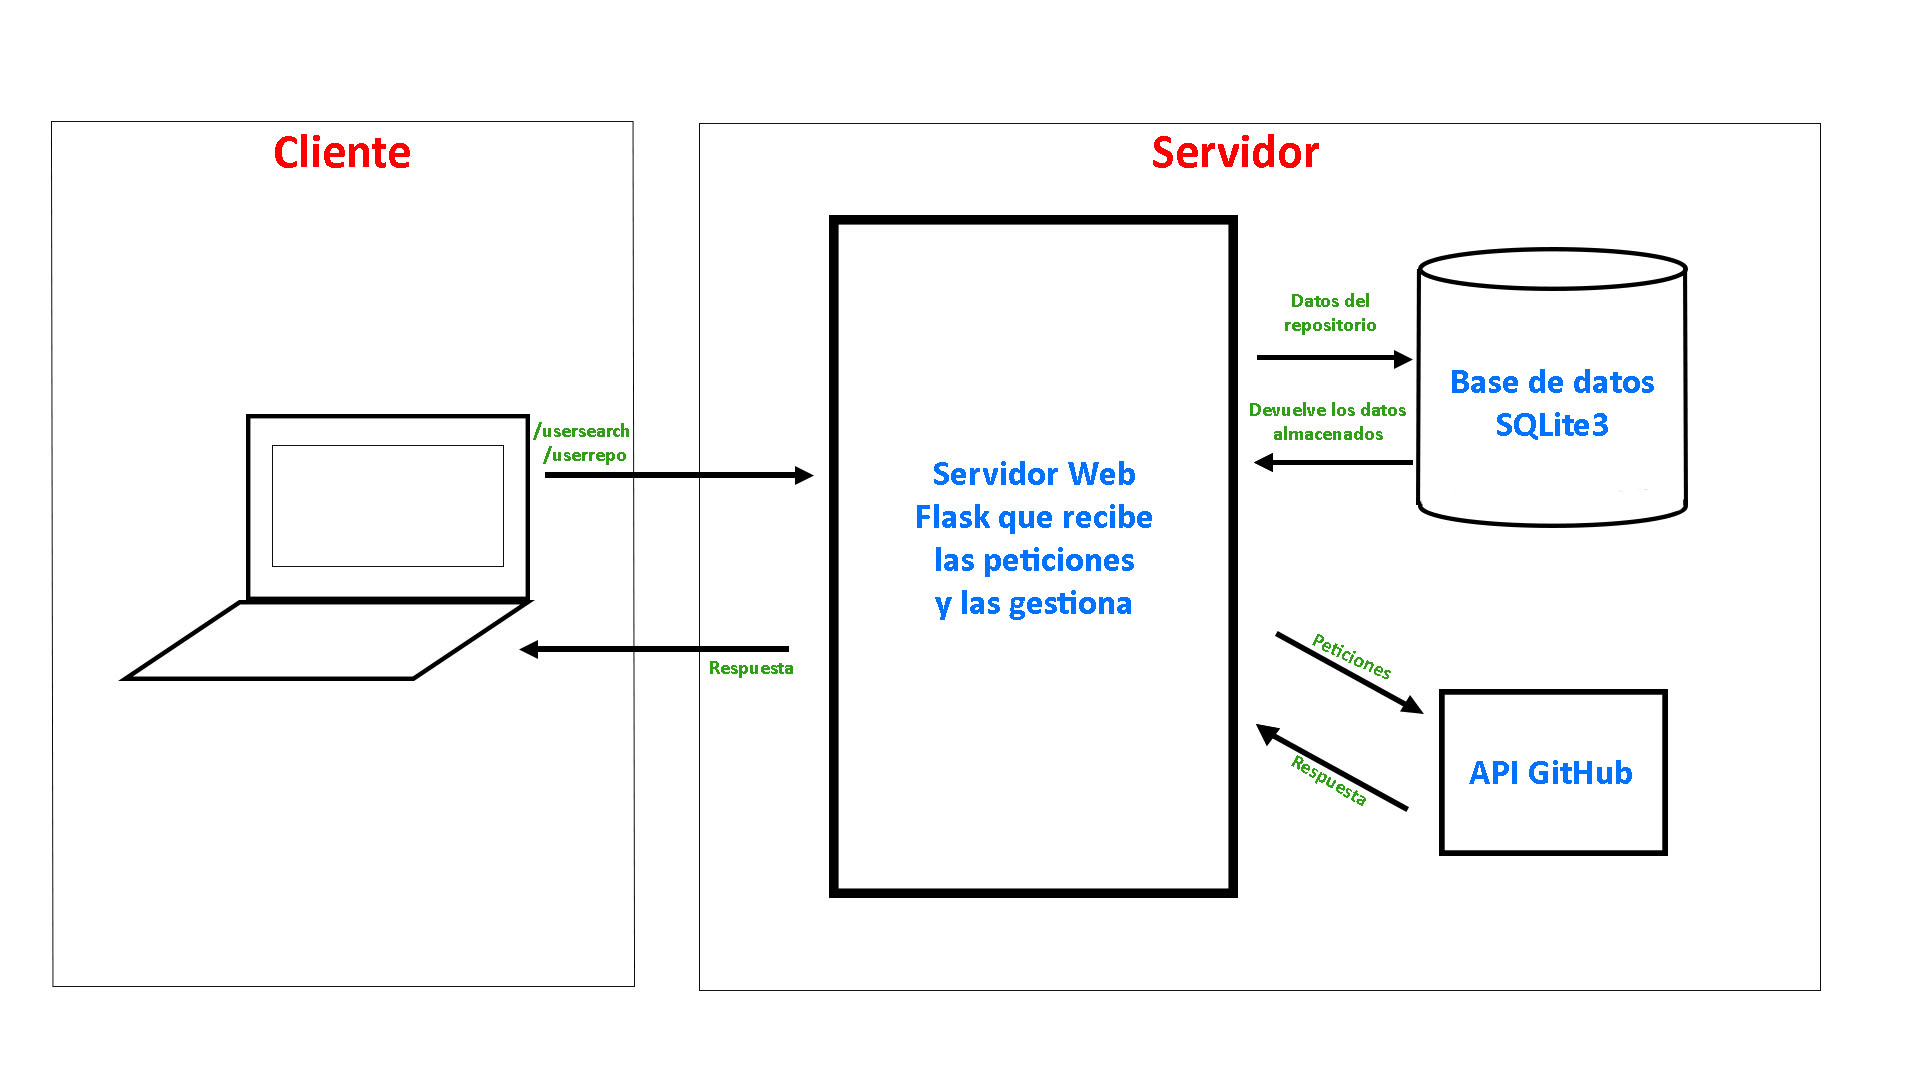
\includegraphics[width=1\textwidth]{img/arquitecturageneralv2.jpg}
  \caption{Arquitectura general de la aplicación}
  \label{figura:arqgeneral}
\end{figure}

Un cliente cualquiera accede a la página web del proyecto, a la que he llamado OSSAnalyzer (viene de Open Source Software Analyzer), y haciendo click en el botón ``Búsqueda de un repositorio concreto'' en el encabezado de la página principal, provoca que el navegador lance una petición GET al endpoint principal de la aplicación (/userrepo). El servidor, después, ofrece en la respuesta un formulario donde el usuario deberá introducir el nombre del repositorio y el nombre del propietario del repositorio, con el objetivo de hacer una petición POST al servidor, también al endpoint /userrepo. Al llamar a este endpoint con estos datos y con el método POST, el servidor realiza toda la parte interna de recolección de datos usando Perceval, realiza también el análisis de los datos obtenidos y además, también realiza la representación de este análisis en la propia aplicación web. No hay que olvidar también la base de datos que forma parte de la aplicación; ya que los datos de los repositorios que se vayan a analizar, es decir, que se vayan a introducir en el endpoint /userrepo se van a guardar en la base de datos para tenerlos almacenados.

Además, está disponible también el endpoint /usersearch, que facilita la búsqueda de los repositorios perteneciente a un usuario que el cliente debe escoger. Esto se hace de manera que con una petición GET, el servidor devuelve al cliente un formulario que debe rellenar con el usuario propietario, y al enviarlo, se realiza una petición POST, con la que el servidor, después de procesarla, le ofrece al cliente la lista de repositorios que posee ese usuario para que posteriormente pueda analizarlos.

\section{Estructura del código del proyecto}
\label{sec:Estructura del código del proyecto}

Para hacer más sencilla la explicación de partes del código en puntos posteriores, hablaré de la estructura de código del proyecto:

\begin{verbatim}

  OSSAnalyzer/
  |---> main.py
  |
  |---> utils.py
  |
  |---> requests_to_github_api.py
  |
  |---> readme.md
  |
  |---> config/
  |     |
  |     |---> OSSAnalyzerConfig.json
  |
  |---> logs/     
  |     |  
  |     |--->OSSAnalyzer.log
  |
  |---> web/
       |
       |---> endpoints.py
       |
       |---> models.py
       |
       |---> __init__.py
       |
       |---> database.db
       |
       |---> static/
       |     |
       |     |---> mainpage.css
       |     |
       |     |---> mainpage.js
       |     |
       |     |---> userrepo.css
       |     |
       |     |---> userrepo.js
       |     |
       |     |---> formulario.css
       |     |
       |     |---> formulario.js
       |     | 
       |     |---> images/
       |          |
       |          |---> logoaplicacion.png
       |
       |---> templates/
             |
             |---> base.html
             |
             |---> mainpage.html
             |
             |---> userrepoForm.html
             |
             |---> userrepoResult.html
             |
             |---> usersearchForm.html
             |
             |---> usersearchResult.html.

\end{verbatim}

\begin{itemize}
  \item \textbf{main.py}: Contiene la información necesaria para arrancar la aplicación.
  \item \textbf{utils.py}: Contiene todas las funciones usadas para la recolección de datos de los repositorios obtenidos usando la librería Perceval. También contiene métodos para calcular los lenguajes minoritarios y los contribuyentes que han participado en los mismos.
  \item \textbf{requests\_to\_github\_api.py}: Contiene todas las funciones usadas para la recolección de datos extra mediante llamadas a la API de GitHub.
  \item \textbf{readme.md}: Es un fichero Markdown con una breve introducción a la aplicación. Se usa sobre todo para que al entrar en la página del repositorio en GitHub, cualquier usuario pueda ver fácilmente de qué trata el proyecto.
  \item \textbf{config/OSSAnalyzerConfig.json}: Es un fichero de configuración en formato JSON que se usa principalmente para guardar configuraciones que sean modificables fácilmente y no haya que cambiar más código si fuera necesario. Contiene información sobre la IP y el puerto donde se inicia la aplicación, configuración de los logs, el token que se usa en todas las llamadas contra la API de GitHub y un diccionario con una gran cantidad de extensiones y el lenguaje que representan.
  \item \textbf{logs/OSSAnalyzer.log}: En este fichero de log se escribe continuamente el estado de la aplicación, las peticiones que llegan y sus resultados, errores e información extra. Realmente este fichero tendría sentido si la aplicación estuviera corriendo en un servidor continuamente, ya que sirve para investigar posibles fallos.
  \item \textbf{web/models.py}: En este fichero se definen los modelos de las tablas con sus correspondientes columnas en la base de datos.
  \item \textbf{web/database.db}: En este fichero se almacena la base de datos SQLite3.
  \item \textbf{web/endpoints.py}: En este fichero se definen todos los endpoints de la aplicación y las acciones que realizan cada uno de ellos.
  \item \textbf{web/\_\_init\_\_.py}: Contiene la información para crear la aplicación y cargar todos los elementos, la base de datos, y los endpoints.
  \item \textbf{web/static}: En este directorio se almacenan las imágenes, y los ficheros CSS y JavaScript de las páginas.
  \item \textbf{web/templates}: Este directorio almacena los ficheros HTML con los templates que se modifican.
\end{itemize}

\section{Comenzando a usar la aplicación}
\label{sec:Empezando a usar la aplicación}

El primer paso para comenzar a usar la aplicación es, obviamente, acceder a la web desde un navegador. Al entrar se presenta una página de inicio en la que se informa al usuario de la finalidad del proyecto y una pequeña guía para facilitar el uso de la aplicación, aunque es bastante sencillo.

El usuario, debe escoger en ese momento entre dos opciones que se dan en el encabezado de la página:

\begin{itemize}
  \item Búsqueda de un repositorio concreto: Llama al endpoint /userrepo de la aplicación usando un método GET.
  \item Búsqueda por usuario: Llama al endpoint /usersearch de la aplicación usando un método GET.
\end{itemize}

\begin{figure}[H]
  \centering
  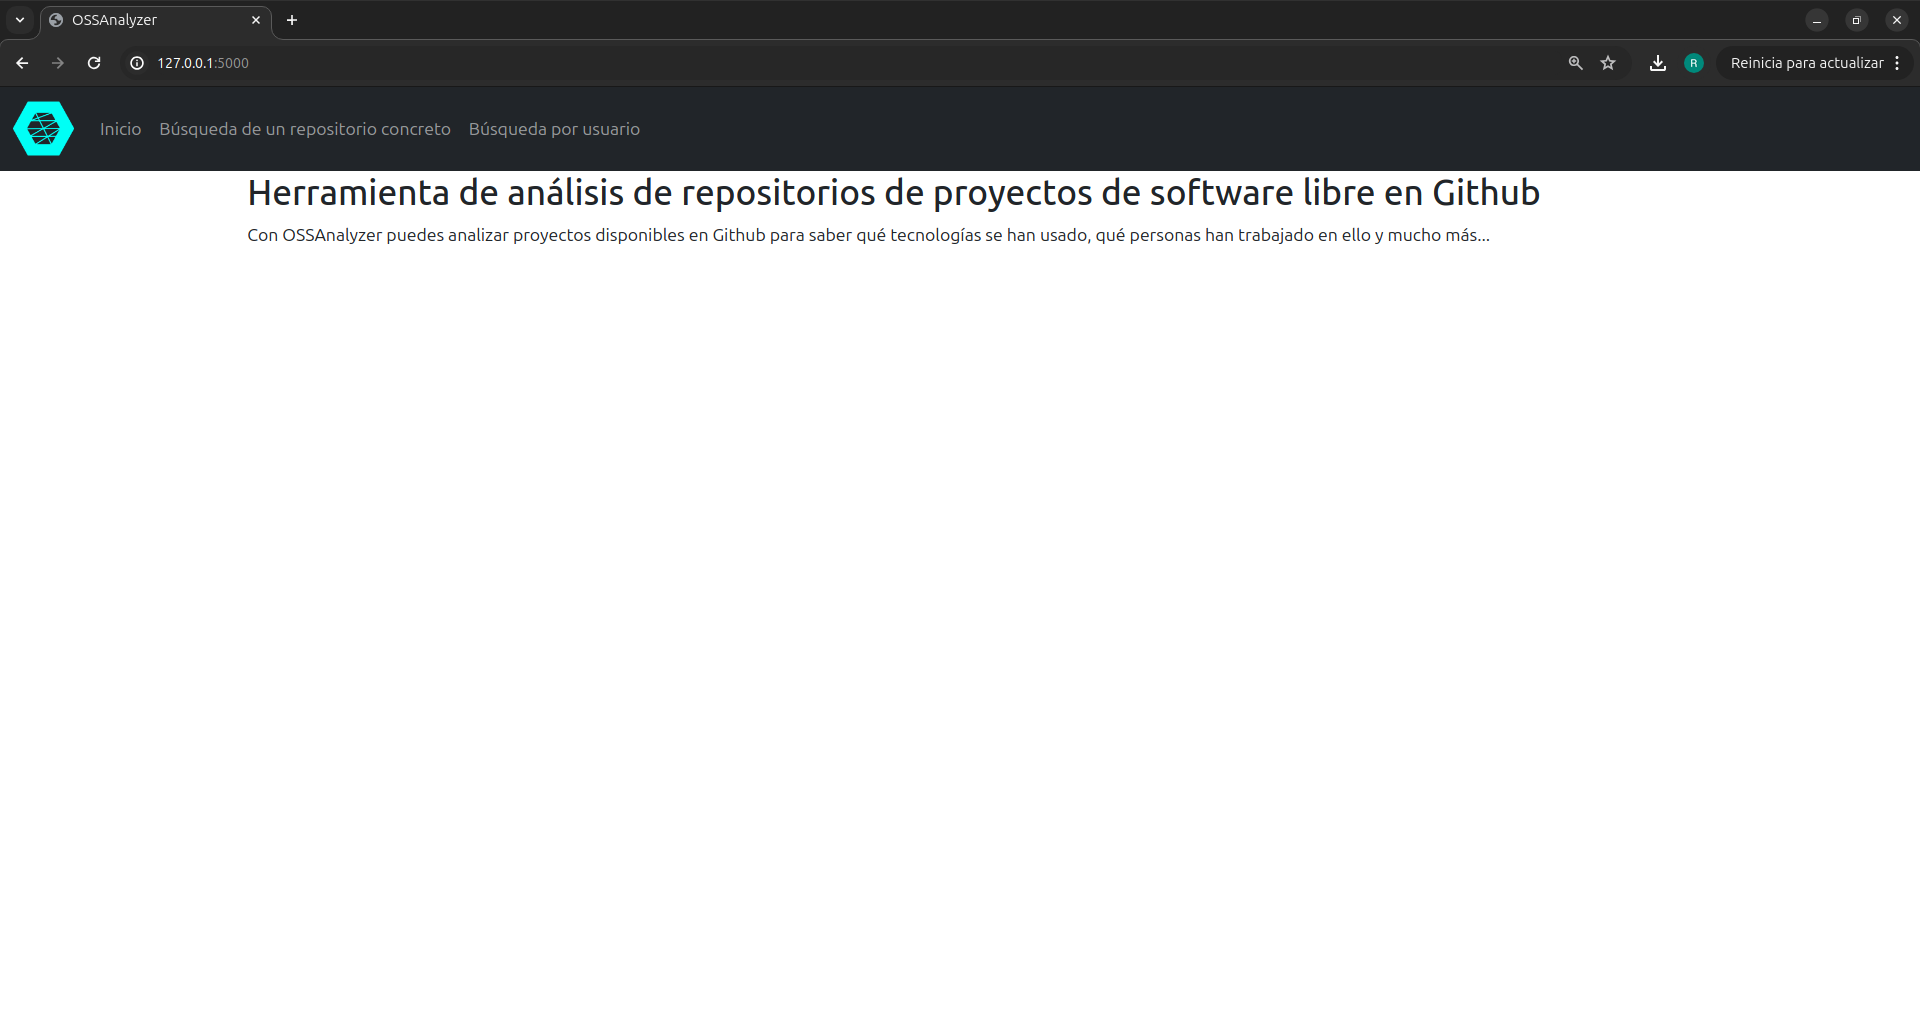
\includegraphics[width=1\textwidth]{img/paginaprincipal.png}
  \caption{Página inicial de la aplicación}
  \label{figura:appmainpage}
\end{figure}


\section{Endpoint /userrepo}
\label{sec:/userrepo}

En el endpoint /userrepo es donde se encuentra la gran mayoría de la lógica de la aplicación.

Al llamar a este endpoint con un método GET, el servidor responde a la petición con un formulario con dos campos que el cliente deberá rellenar: el nombre del repositorio, y el nombre del propietario del repositorio. También, se entrega en la respuesta un botón de envío, que al pulsarlo, provoca que el navegador lance una petición al endpoint /userrepo, pero ahora usando un método POST. Al ser una petición POST, los parámetros se encuentran en el body, y en este caso son dos: username (nombre de usuario del propietario del repositorio) y repo (nombre del repositorio).


\begin{figure}[H]
  \centering
  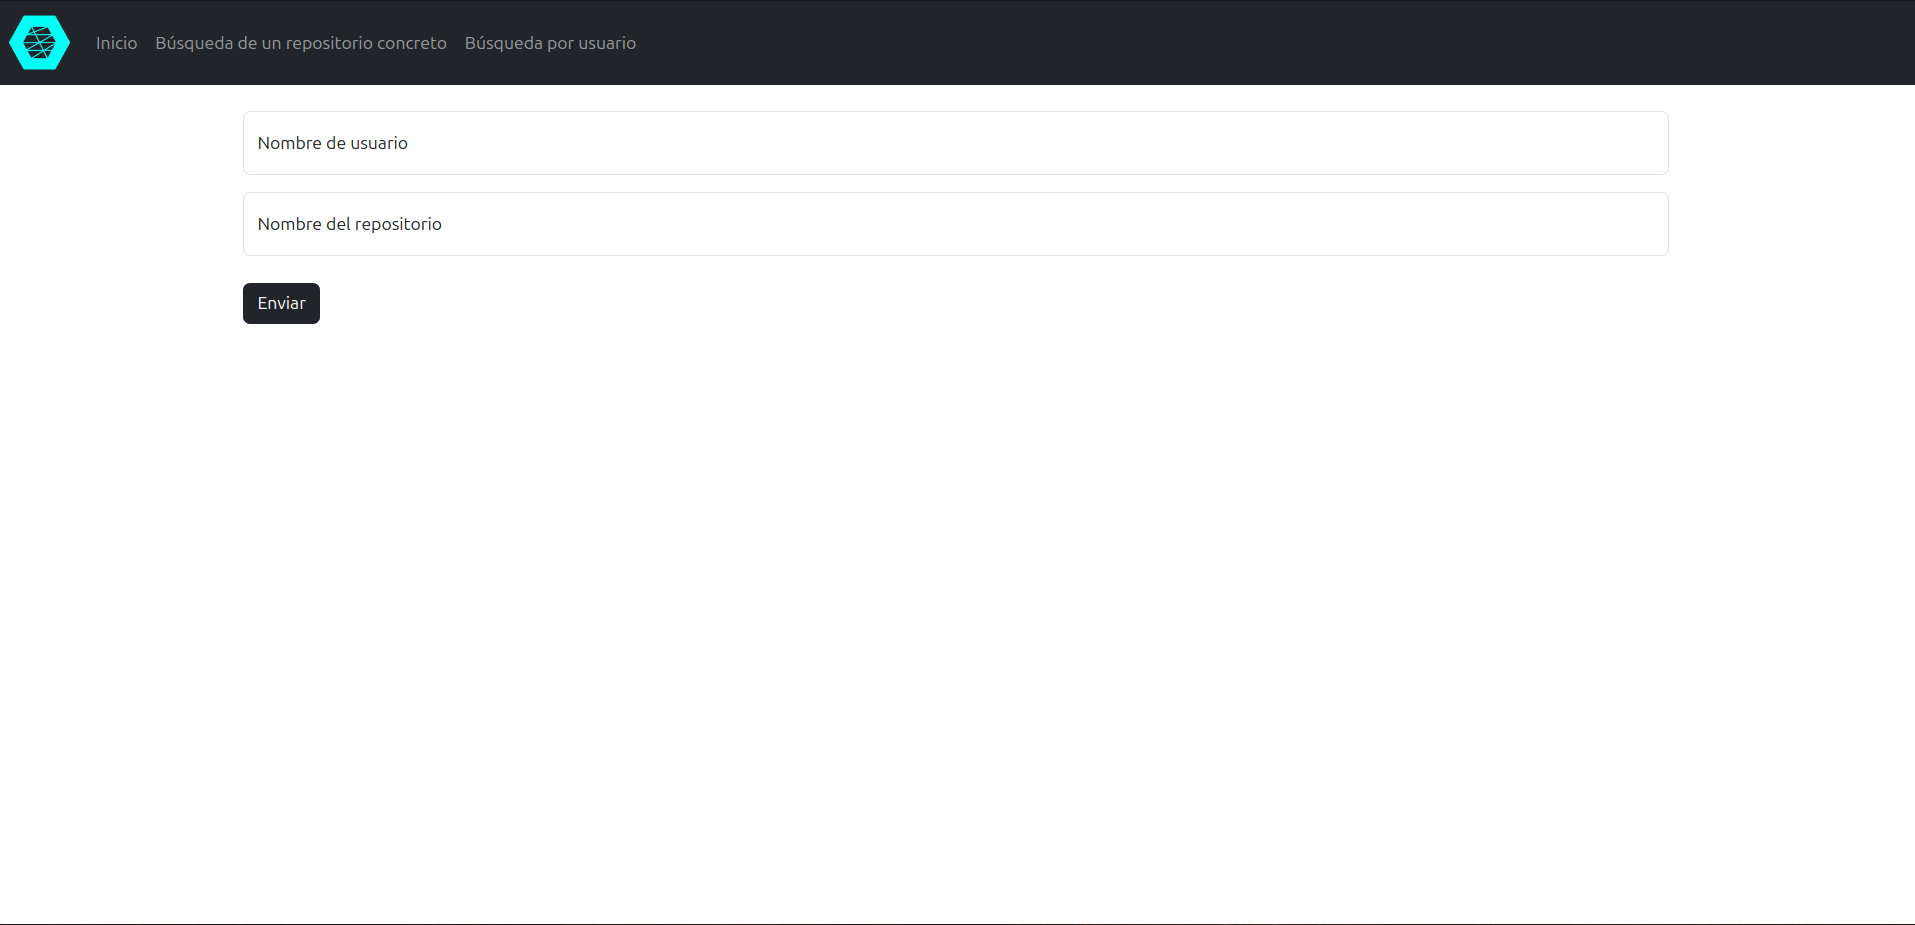
\includegraphics[width=1\textwidth]{img/userrepoget.png}
  \caption{Respuesta con el formulario a la petición con método GET}
  \label{figura:userrepoget}
\end{figure}
Una vez que llega al servidor esa petición POST, comienza la lógica del análisis del repositorio que el usuario ha escogido:

La primera tarea que realiza el servidor es la obtención de la rama por defecto del repositorio y el identificador del último commit que se ha subido en esa misma rama. El sentido de esto tiene que ver con la implementación con la base de datos, ya que desde un punto de vista de rendimiento, no tendría sentido guardar de nuevo en la base de datos un repositorio cuya última versión ya tenemos almacenado. La comprobación que realiza el servidor para saber si ese repositorio ya está almacenado en la base de datos se hace mediante una consulta contra la base de datos. Si ese repositorio no está almacenado, o si la fecha del último commit es anterior a la que se ha obtenido anteriormente, se procede con la recolección de datos del repositorio.

\begin{figure}[H]
  \centering
  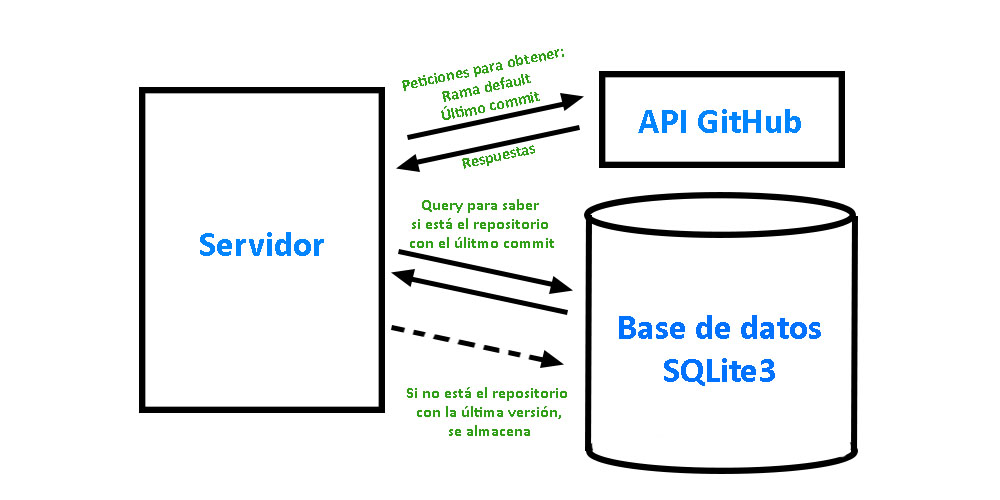
\includegraphics[width=1\textwidth]{img/flujo1.jpg}
  \caption{Flujo de la aplicación para consultar si existe la última versión de un repositorio en la base de datos}
  \label{figura:flujoconsulta}
\end{figure}


Como hemos comentado en puntos anteriores, la recolección de datos de los repositorios se ha hecho usando la libería Perceval. Perceval nos permite obtener todos los datos de los commits realizados sobre un repositorio Git en formato JSON, lo que facilita después la selección de datos que nos interesan, y descartar aquellos datos inservibles para nuestro análisis.



Los datos que podemos sacar del uso de Perceval y que nos interesan en nuestro análisis principalmente, son:

\begin{itemize}
  \item Lista de usuarios que han realizado commits sobre el repositorio: para ello se ha creado la función obtain\_users en utils.py, que genera esta lista accediendo al campo Author de cada uno de los objetos (cada uno de los objetos representa un commit) del JSON obtenido del uso de Perceval.
  \item Obtener los ficheros que ha modificado cada uno los usuarios de la lista creada anterior: usando la función obtain\_users\_files de utils.py, se genera un diccionario de listas con los archivos en los que ha trabajado cada usuario que ha participado en el repositorio.
  \item Obtener las extensiones de los ficheros que ha modificado cada usuario para conocer el lenguaje sobre el que se han hecho las modificaciones: con la función obtain\_files\_extension del fichero utils.py se logra crear un diccionario con los lenguajes. Para ello se usa un diccionario llamado extensiones que se encuentra almacenado en un fichero de configuración JSON (OSSAnalyzerConfig.json). En este diccionario de extensiones se almacena como clave la extensión, y como valor el lenguaje de programación. Para la construcción de este diccionario se ha usado el fichero YAML languages.yml del repositorio Linguist de GitHub, que contiene una gran cantidad de lenguajes.
  \item Obtener el total de modificaciones realizadas sobre un mismo lenguaje de programación de cada uno de los contribuyentes al repositorio: para ello se ha creado la función counter\_ext, almacenada también en utils.py y cuya salida consiste en un diccionario con la suma de modificaciones realizadas sobre todos los lenguajes que cada uno de los usuarios ha realizado.
\end{itemize}

Además para enriquecer algo más el análisis y ofrecer otros datos que no podemos obtener usando Perceval, se han incluido también algunas llamadas a la API de GitHub para obtener los siguientes datos:

\begin{itemize}
  \item Porcentaje de uso de cada uno de los lenguajes usados en el repositorio. Mediante la función obtain\_used\_languages\_on\_repo del fichero requests\_to\_github\_api.py se obtienen todos los ficheros almacenados en el repositorio. Una vez tenemos la lista con todos los ficheros, usando su extensión, se convierte a "lenguaje" de igual manera que se hace con los datos que hemos obtenido de Perceval anteriormente, es decir, usando el diccionario extensiones del fichero de configuración OSSAnalyzerConfig.json. Con ello ya tenemos el total de ficheros de cada lenguaje, por lo que es fácil obtener el porcentaje de cada uno de los lenguajes sobre el total.
  \item Número total de ficheros del repositorio. Se obtiene usando la función obtain\_num\_files del fichero requests\_to\_github\_api.py.
\end{itemize}

Por último, para terminar nuestra recolección de datos, puesto que nos centramos en los lenguajes minoritarios, necesitamos saber qué lenguajes son minoritarios en un repositorio, y la información sobre los mismos. Entendemos que un lenguaje es minoritario en un repositorio si representa una cuota menor del 5\% del total de un repositorio. Por ejemplo:

Un repositorio contiene 5 lenguajes de programación: Python, HTML, CSS, JavaScript y un Dockerfile. Python representa el 80\% del repositorio, HTML un 10\%, CSS un 7\%, JavaScript, un 2\% y Dockerfile, el 1\% restante. En este caso, los lenguajes minoritarios serán JavaScript y Dockerfile.

Teniendo esto en mente, debido a que se obtiene el porcentaje de uso de cada uno de los lenguajes usado en los repositorios como se ha comentado anteriormente, se puede saber cuales de los lenguajes que forman parte de un repositorio son minoritarios. Ahora que tenemos los lenguajes minoritarios, buscamos el resto de información sobre estos: los commits hechos sobre esos lenguajes y quién de los usuarios contribuyentes han realizado estos commits.

Todo esto se hace de la siguiente manera:

\begin{itemize}
  \item Obtención de los lenguajes minoritarios: con el diccionario de porcentajes de cada uno de los lenguajes de un repositorio, usando la función obtain\_min\_languages del fichero utils.py nos quedamos con una lista con solo los lenguajes que representan menos del 5\% que hemos definido.
  \item Número total de commits realizados sobre esos lenguajes minoritarios: se realiza un diccionario en el que se hace la suma total de commits realizados sobre cada lenguaje minoritario usando la lista anterior y los datos que hemos obtenido de los commits con Perceval con el total de modificaciones realizadas cada uno de los lenguajes por cada contribuyente al repositorio. Esta función la realiza el método obtain\_total\_commits\_min\_languages del fichero utils.py.
  \item Obtención de los contribuyentes y su participación en los lenguajes minoritarios: mediante la función top\_contribuyebtes\_por\_lenguaje del fichero utils.py se construye un diccionario con el número de commits realizados por los usuarios que han contribuido en estos lenguajes.
\end{itemize}

Ya se tienen todos los datos necesarios para nuestro análisis, por tanto, se procede a su almacenamiento en la base de datos.

En caso de que el repositorio no esté almacenado,se crea una fila en la tabla Repository de la base de datos con diferentes columnas con cada uno de los datos de interés para el análisis. El otro caso que se puede dar es que el repositorio que se haya analizado sea uno que ya existía en la tabla Repository, pero de una versión posterior, por lo que en lugar de crear una nueva fila, se actualizan las columnas de la fila ya existente, de manera que no se gasta espacio innecesario en la base de datos.

\begin{figure}[H]
  \centering
  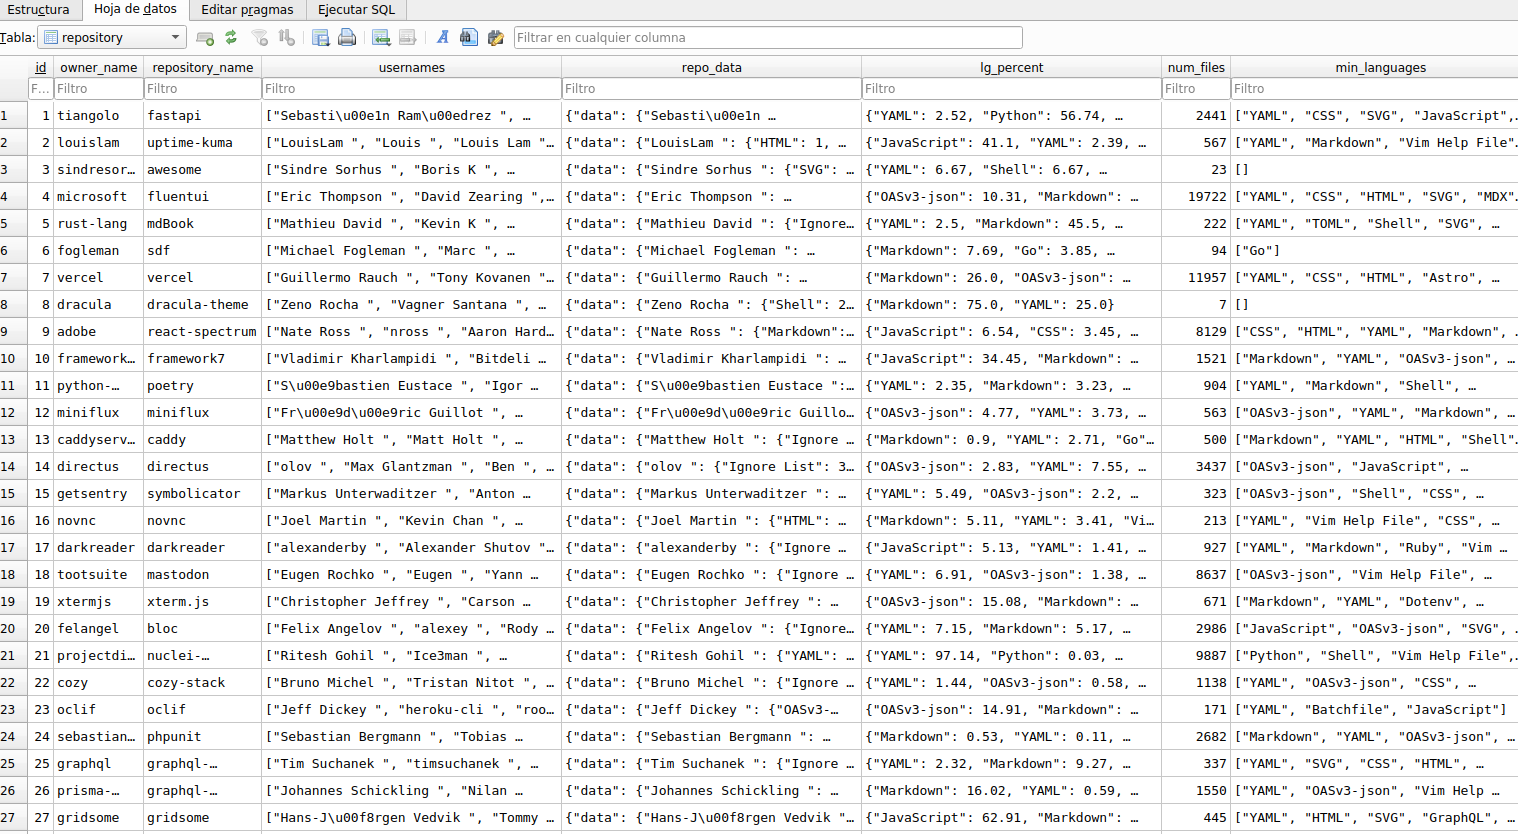
\includegraphics[width=1\textwidth]{img/tablarepository.png}
  \caption{Tabla Repository}
  \label{figura:tablarepo}
\end{figure}

También, además de almacenar cada repositorio en la tabla Repository, se guardan todos los usuarios que han participado en cada uno de los repositorios analizados junto a los repositorios que ha participado y los commits que ha realizado en los mismos. Esto nos permite ver el expertise de cada uno de los usuarios y conocer en qué lenguaje se especializa y qué número de lenguajes totales ha usado en todos los repositorios que haya participado y se hayan analizado previamente en la aplicación. Todo esto se almacena en la tabla User\_expertise de la base de datos.

\begin{figure}[H]
  \centering
  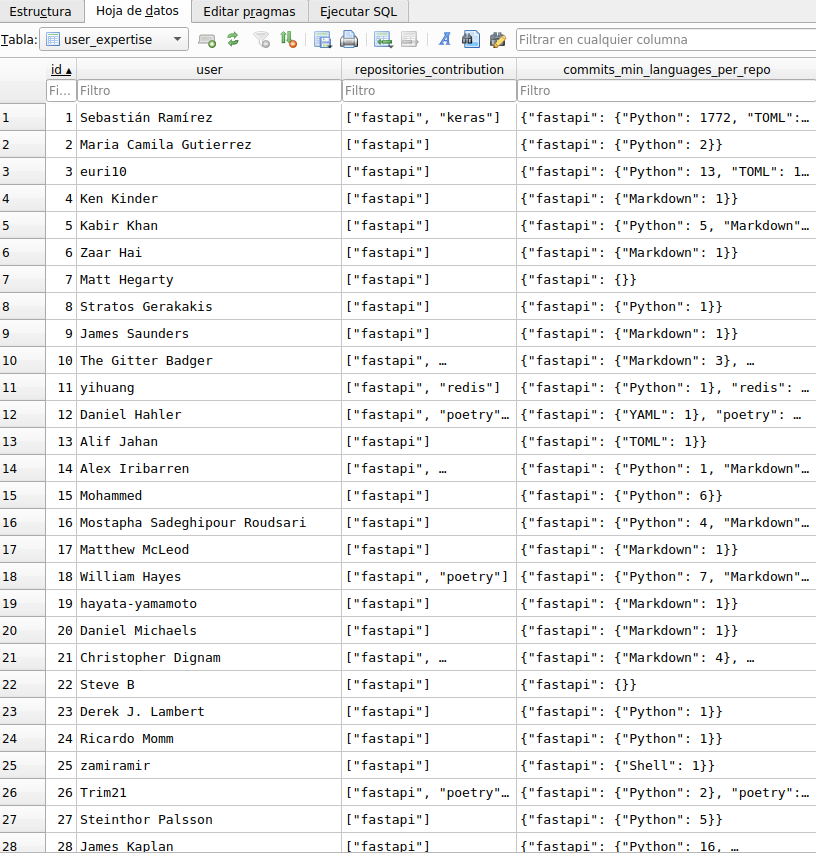
\includegraphics[width=1\textwidth]{img/tablauser_expertise.png}
  \caption{Tabla User\_expertise}
  \label{figura:tablaue}
\end{figure}

Por último, se almacenan los datos de los distintos lenguajes que han formado ese repositorio. Para ello, se crea un diccionario usando los datos obtenidos con Perceval cuyas claves son los lenguajes, y los valores son una lista con el número de commits totales realizados, el número de usuarios que ha hecho commits sobre ese lenguaje, y la lista de usuarios que hayan hecho los commits. Se almacenan en la tabla Languages.

\begin{figure}[H]
  \centering
  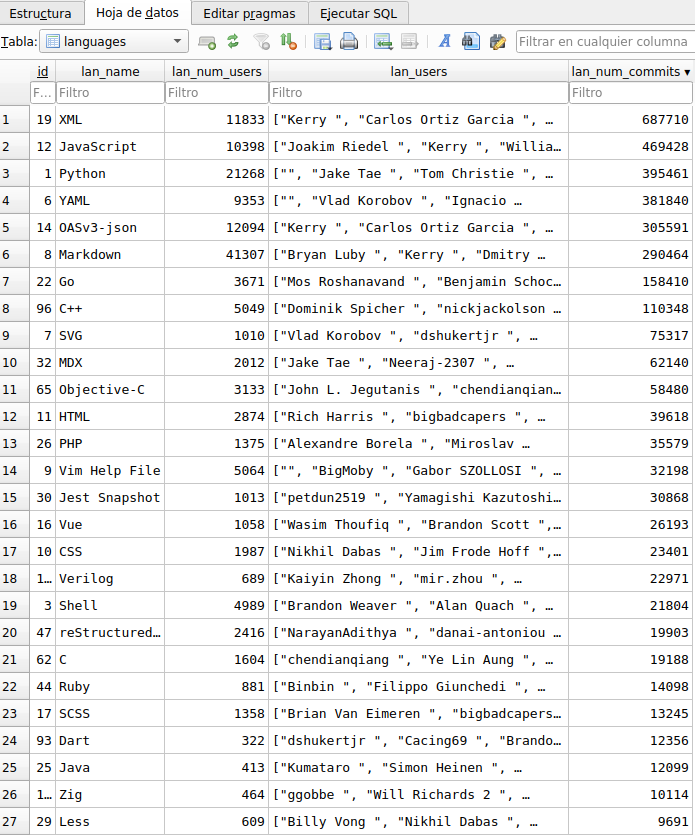
\includegraphics[width=1\textwidth]{img/tablalanguages.png}
  \caption{Tabla Languages}
  \label{figura:tablalang}
\end{figure}

Una vez almacenados los distintos datos, solo queda la representación de los mismos en la aplicación web. Se presenta de la siguiente manera:

\begin{figure}[H]
  \centering
  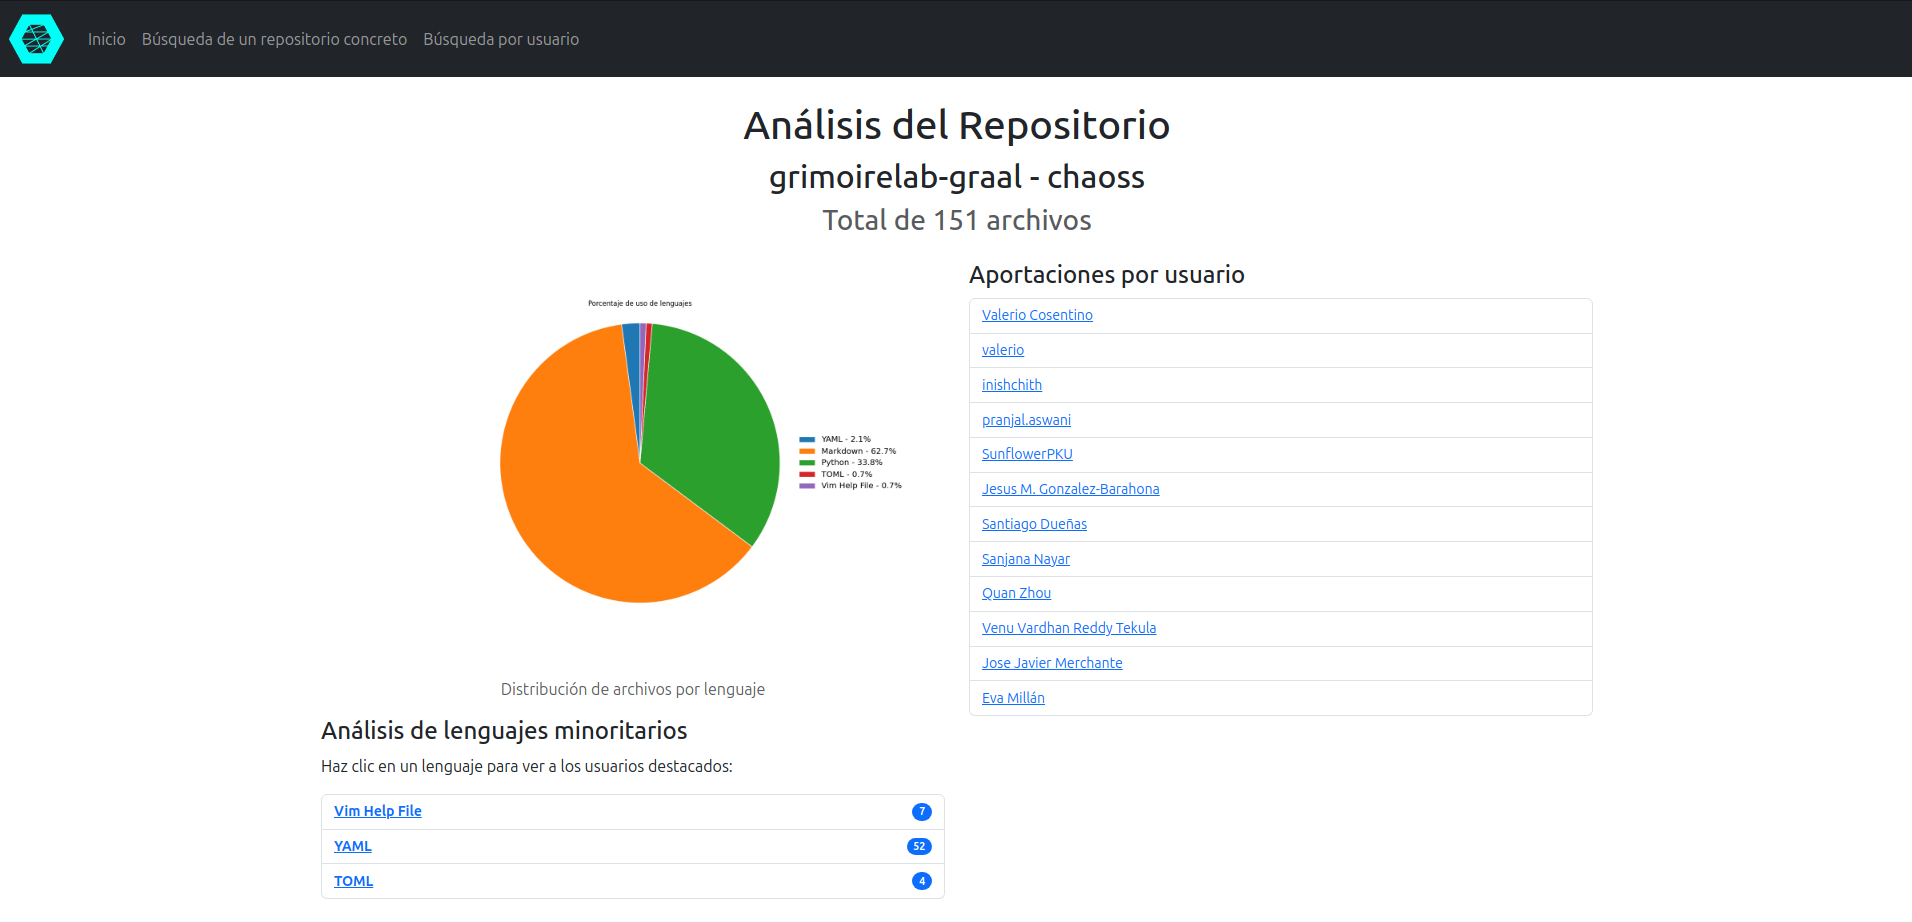
\includegraphics[width=1\textwidth]{img/resultadouserrepo.png}
  \caption{Respuesta a la petición POST con la representación gráfica del análisis}
  \label{figura:resultuserrepo}
\end{figure}

Se informa al usuario del repositorio que se ha pedido analizar y el total de ficheros que tiene el repositorio.

Se presenta una gráfica circular con la representación de porcentaje de cada uno de los lenguajes usados junto a una leyenda para inforar al usuario del número de porcentaje y el color que representa. La gráfica se genera a partir del diccionario con el porcentaje de uso de cada uno de los lenguajes usados en el repositorio que se ha obtenido en la recolección de datos usando la librería Matplotlib. Además, se presentan los lenguajes minoritarios del repositorio y el número de commits totales realizados sobre cada uno de ellos. Si se pulsa en cualquiera de ellos, muestra a los usuarios que han realizado los commits y la cantidad.

\begin{figure}[H]
  \centering
  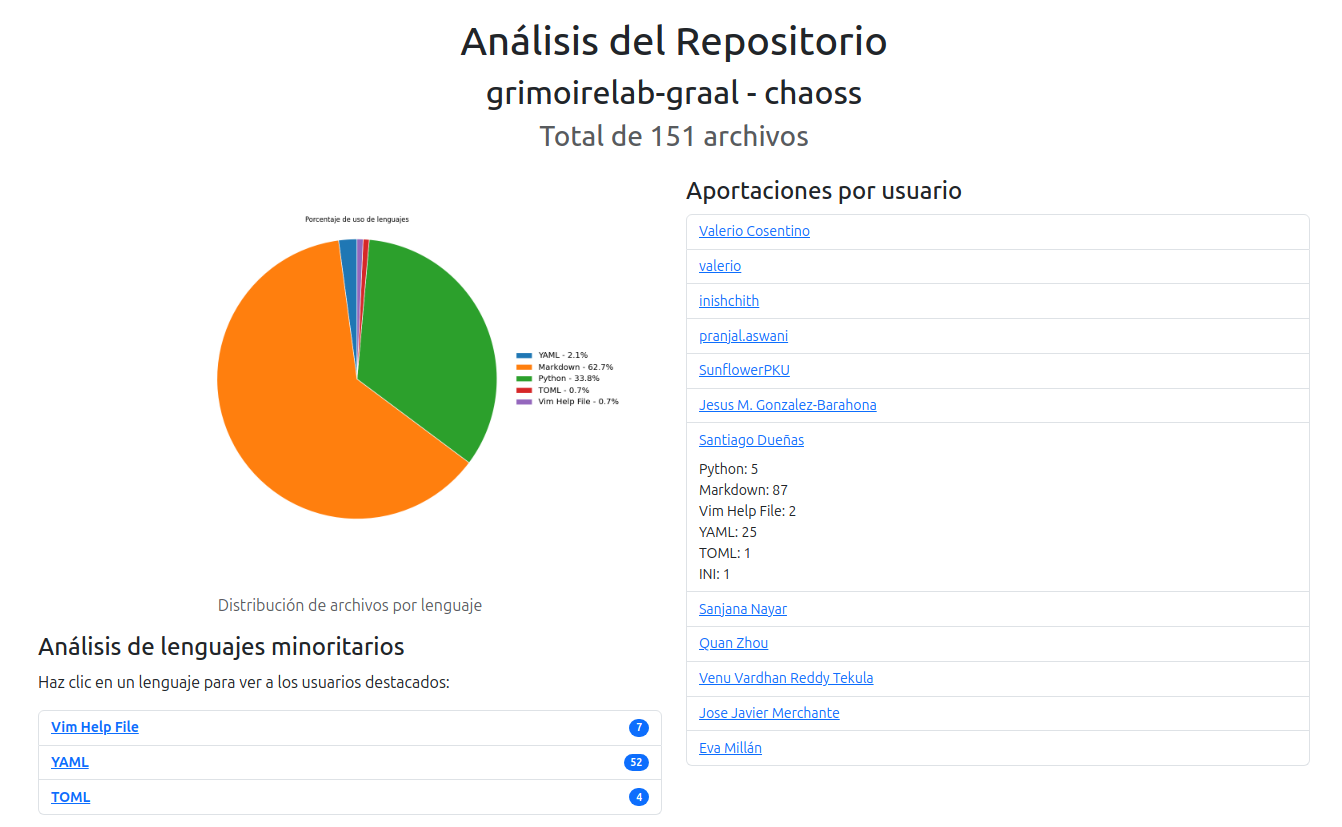
\includegraphics[width=1\textwidth]{img/resultado2userrepo.png}
  \caption{Análisis de los lenguajes minoritarios}
  \label{figura:resultuserrepo2}
\end{figure}

Además, se muestran todos los usuarios que han contribuido, y al hacer clic sobre cualquiera de ellos, muestra los commits realizados sobre cada uno de los lenguajes del repositorio.
\begin{figure}[H]
  \centering
  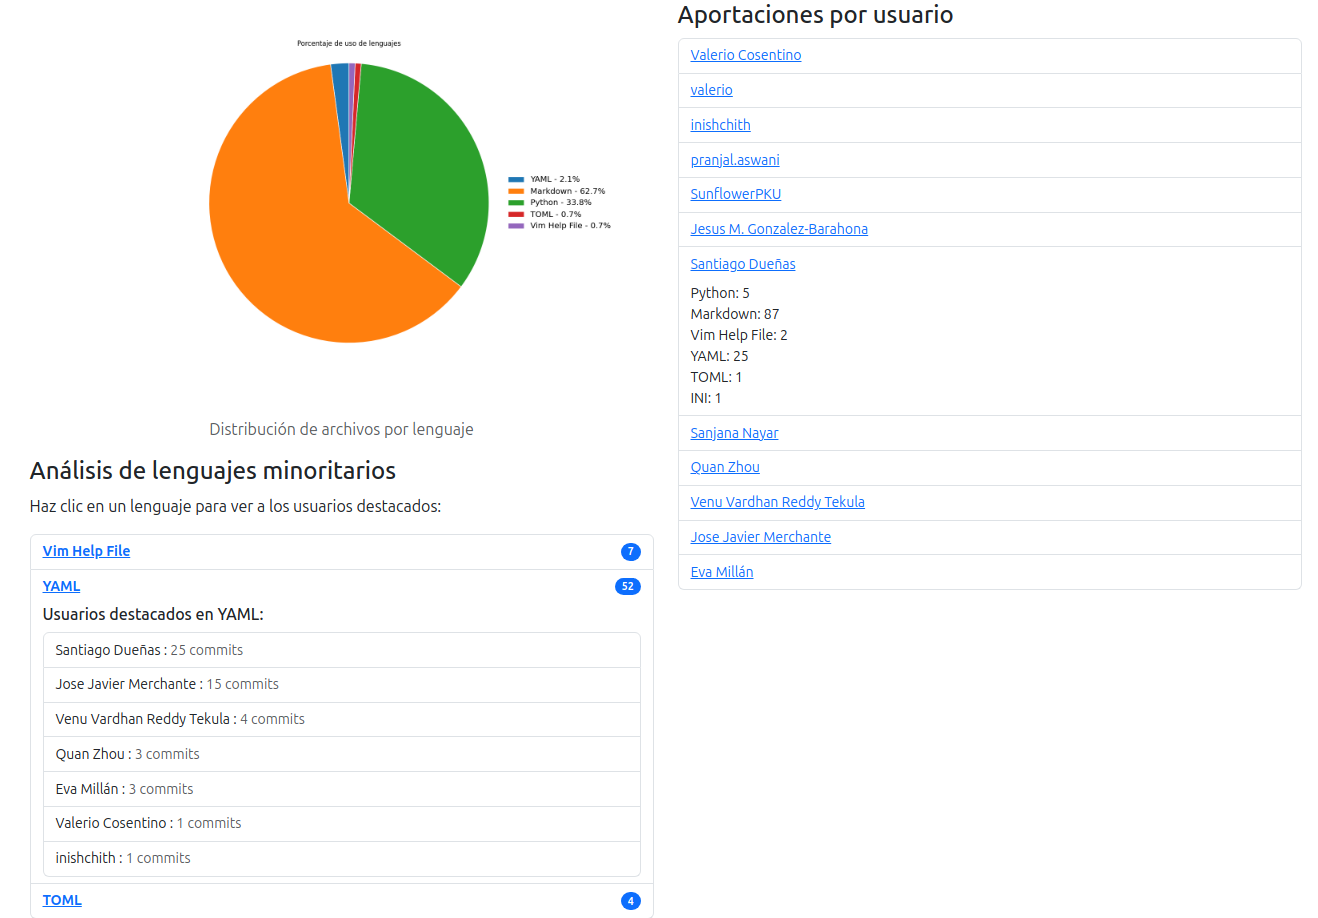
\includegraphics[width=1\textwidth]{img/resultado3userrepo.png}
  \caption{Contribuyentes al repositorio}
  \label{figura:resultuserrepo3}
\end{figure}
Por otro lado, si el repositorio que el usuario pide analizar ya tiene los datos de la última versión almacenada en la base de datos, estos se recuperan mediante una consulta en la que se pide a la tabla Repository la fila correspondiente al repositorio, y con ella se recuperan de nuevo todos los datos para representarlos en la web.

\section{Endpoint /usersearch}
\label{sec:/usersearch}

El objetivo del endpoint /usersearch es facilitar al usuario todos los repositorios públicos que pertenecen a un mismo propietario de manera que pueda localizar fácilmente los repositorios de un mismo usuario sobre los que hacer los análisis de lenguajes minoritarios. Sobre todo, está dirigido de cara a usuarios propietarios que consistan en un grupo de personas que suelen participar en los mismos proyectos.

El funcionamiento es de la siguiente manera:

\begin{itemize}
  \item En caso de que llegue una petición al endpoint con método GET, se ofrece en la respuesta un formulario donde el usuario debe indicar el nombre de usuario de GitHub del cual quiera consultar los repositorios junto a un botón de envío para provocar el envío de una petición al mismo endpoint /userrepo, pero en este caso, con método POST cuyo cuerpo contiene un parámetro llamado username y su valor es lo que haya intoducido el usuario.
    \begin{figure}[H]
      \centering
      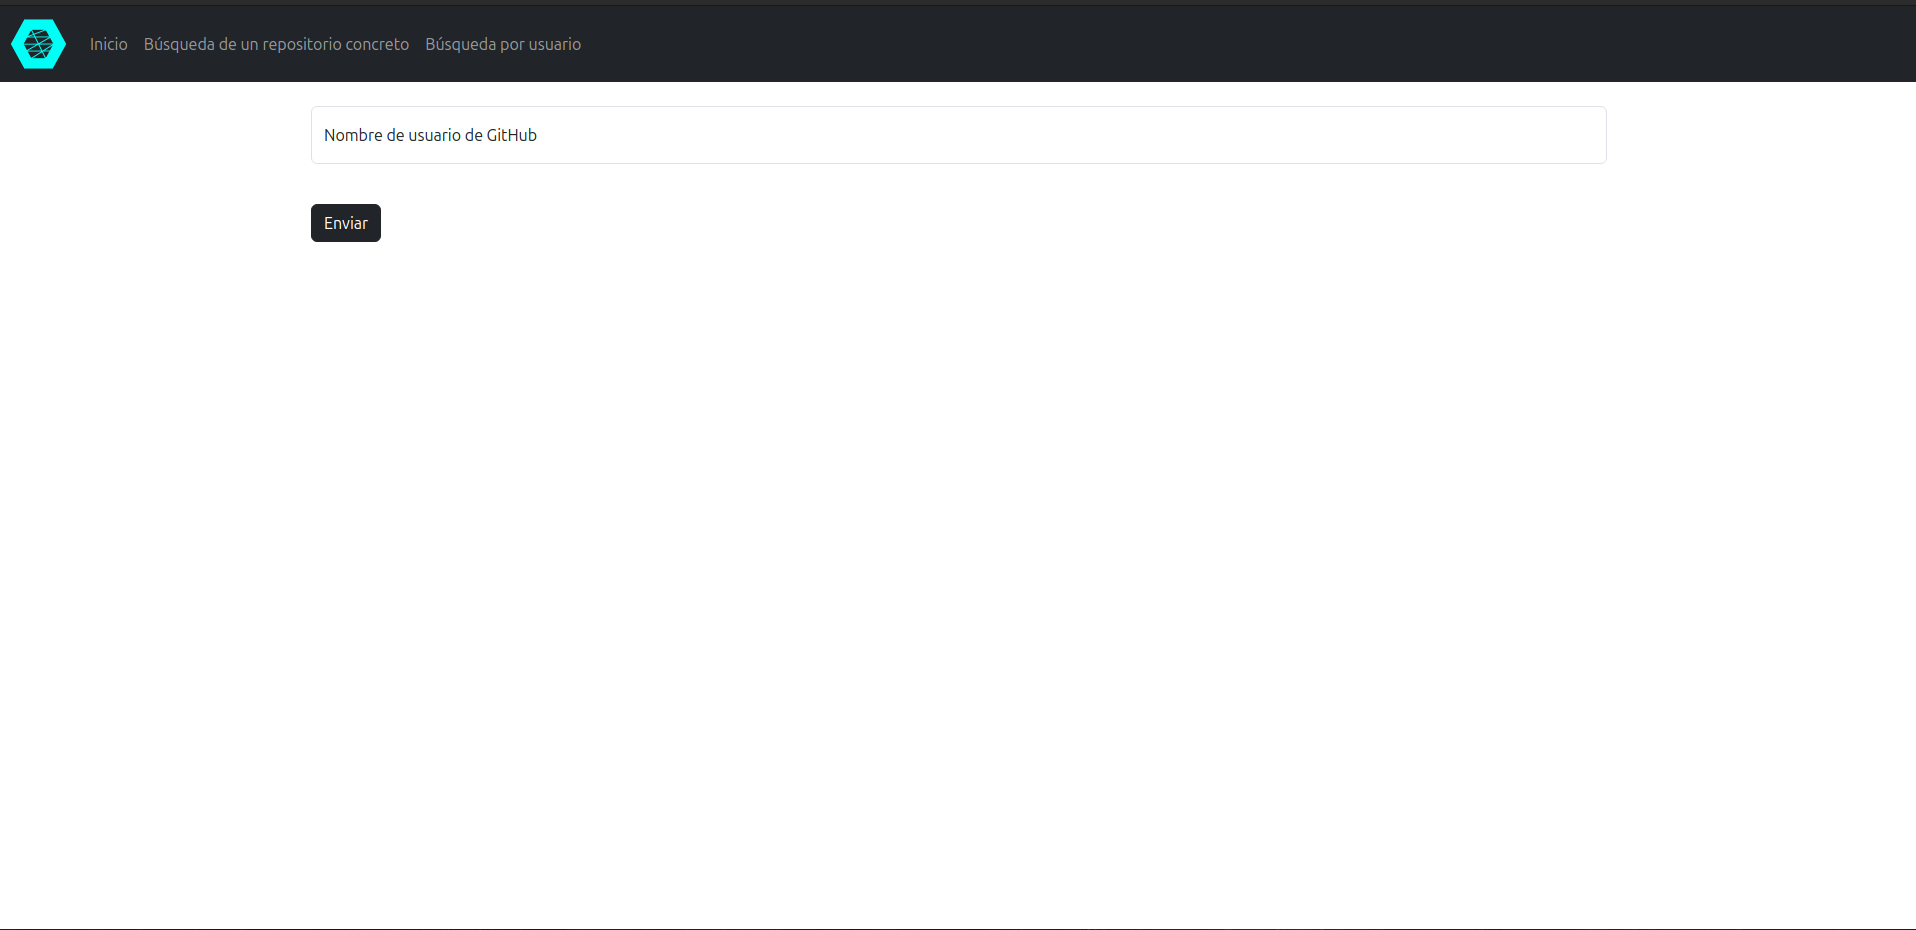
\includegraphics[width=1\textwidth]{img/usersearchget.png}
      \caption{Respuesta a la petición GET al endpoint /usersearch}
      \label{figura:usersearch}
    \end{figure}
  \item Cuando llega esa petición POST, el servidor procede a buscar los repositorios públicos del usuario que ha llegado en el body de la petición. Esto se hace mediante la función obtain\_user\_repos del fichero requests\_to\_github\_api.py, cuya salida es un diccionario con el nombre de todos los repositorios que posee ese usuario. Este diccionario es lo que da forma a la respuesta final del endpoint.
\end{itemize}

Al finalizar, se representa de la siguiente manera en la aplicación web:


\begin{figure}[H]
  \centering
  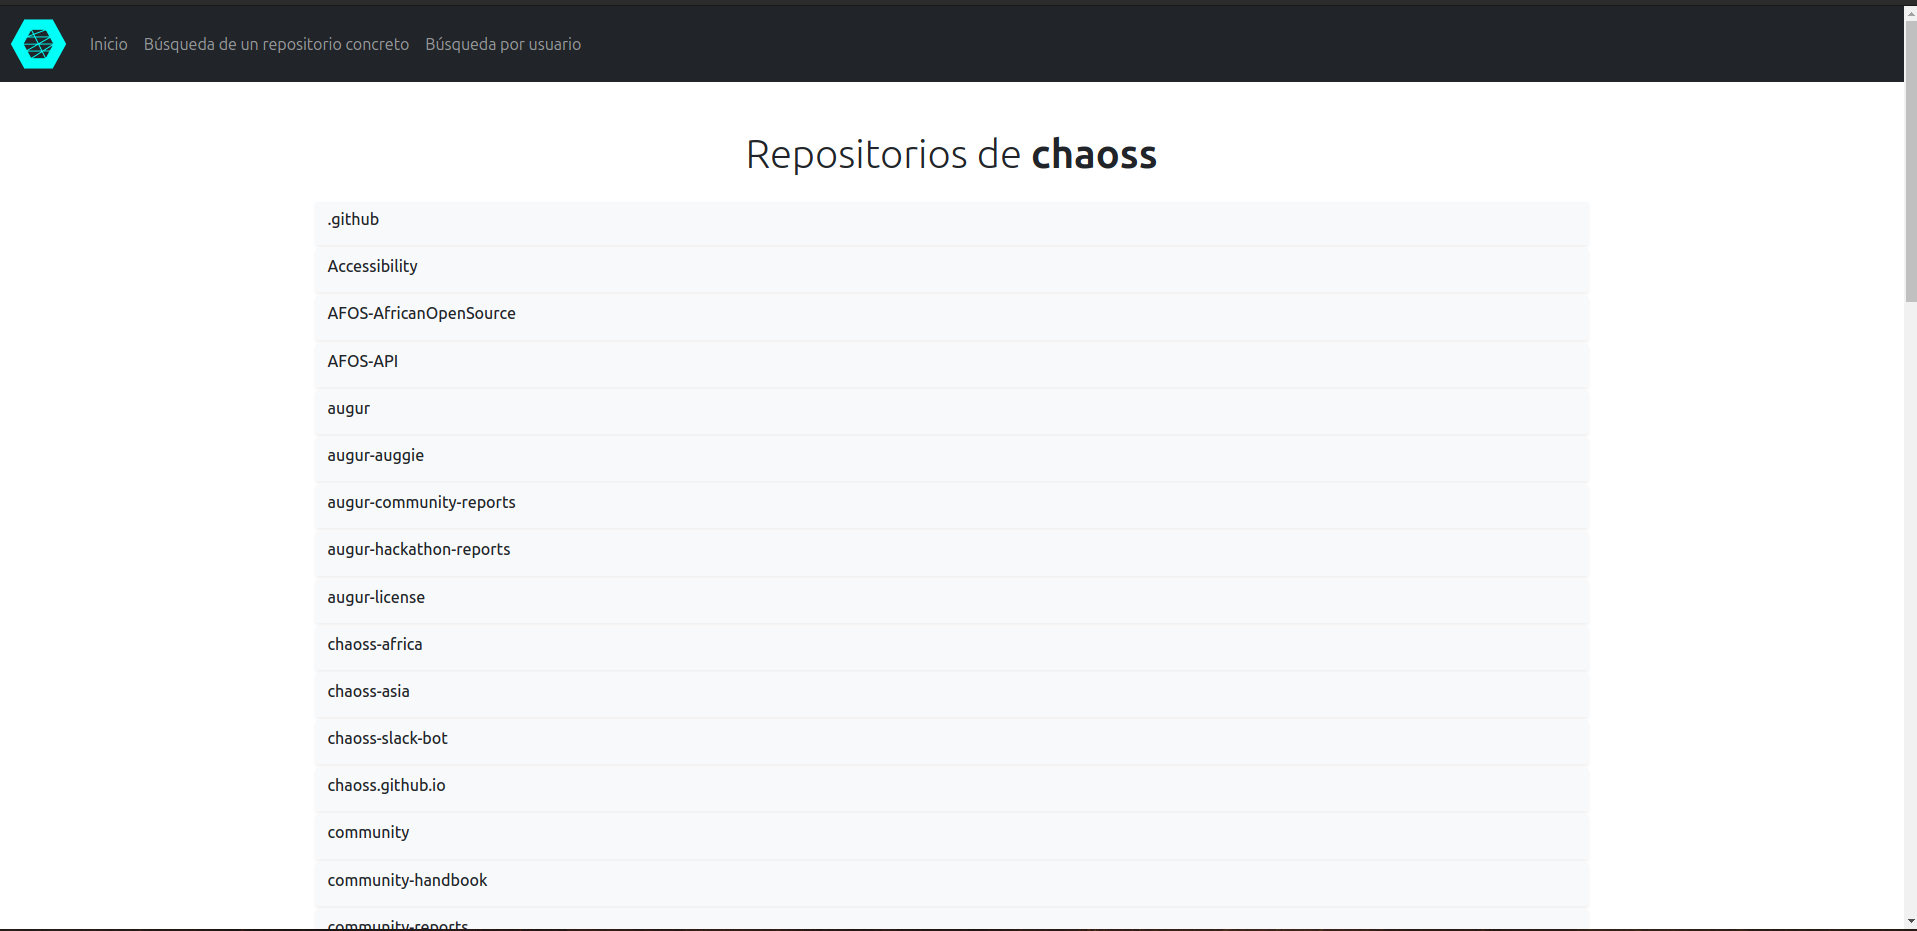
\includegraphics[width=1\textwidth]{img/usersearchpost.png}
  \caption{Respuesta a la petición POST al endpoint /usersearch}
  \label{figura:resultusersearch}
\end{figure}

En la parte superior se informa al usuario del nombre de usuario que ha escogido.

En la parte inferior se muestran todos los repositorios públicos del usuario.

Lo que hace que facilite al usuario la experiencia de analizar varios repositorios de un mismo usuario es que, al clickar en cualquiera de los repositorios que aparecen en la lista, se realiza una llamada POST al endpoint /userrepo con el nombre de usuario y el nombre del repositorio. Como se ha explicado en el punto anterior, en el endpoint /userrepo es donde se realizan los análisis.

\section{Interacción con la base de datos}
\label{sec:Interacción con la base de datos}

Como se ha dicho anteriormente, es la base de datos está basada en SQLite3. Se han definido tres tablas en la base de datos:

\begin{figure}[H]
  \centering
  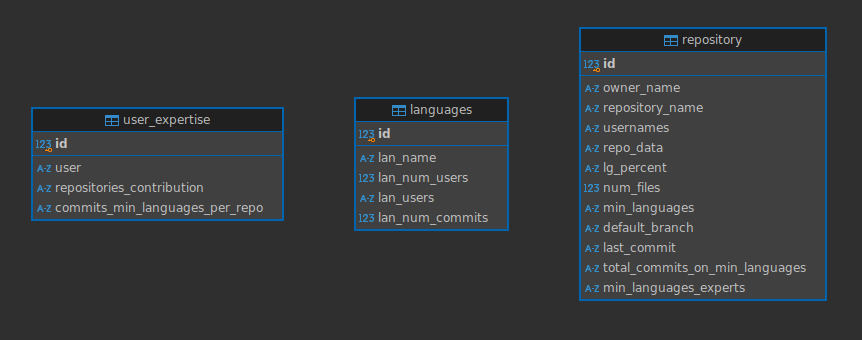
\includegraphics[width=1\textwidth]{img/erdiagram.png}
  \caption{Diagrama entidad-relación de la base de datos}
  \label{figura:Diagrama entidad-relación de la base de datos}
\end{figure}

\subsection{Tabla Repository}
\label{subsec:Tabla Repository}

En la tabla Repository se almacenan los datos de los análisis de los repositorios. Se crea una fila por cada uno de ellos. Las columnas y datos que se guardan son:
\begin{itemize}
  \item \textbf{id}: Identificador interno del repositorio en la base de datos.
  \item \textbf{owner\_name}: Nombre de usuario propietario del repositorio.
  \item \textbf{repository\_name}: Nombre del repositorio.
  \item \textbf{usernames}: Lista de los contribuyentes al repositorio.
  \item \textbf{repo\_data}: Diccionario con los commits que ha realizado cada usuario sobre cada uno de los lenguajes.
  \item \textbf{lg\_percent}: Diccionario con los porcentajes de uso de los lenguajes.
  \item \textbf{num\_files}: Número total de ficheros del repositorio.
  \item \textbf{min\_languages}: Lista con los lenguajes minoritarios.
  \item \textbf{default\_branch}: Nombre de la rama por defecto del repositorio en GitHub.
  \item \textbf{last\_commit}: Identificador del último commit realizado antes del análisis.
  \item \textbf{total\_commits\_on\_min\_languages}: Almacena un diccionario con el número de commits realizados sobre cada uno de los lenguajes minoritarios.
  \item \textbf{min\_language\_experts}: Diccionario con los lenguajes minoritarios, y la cantidad que ha contribuido cada uno de los usuarios que han realizado commits sobre los mismos.
\end{itemize}

\subsection{Tabla User\_expertise}
\label{subsec:Tabla User\_expertise}

Tiene como objetivo obtener información general de todos los usuarios, de cara a saber las tecnologías que conoce cada una de las personas y de qué manera ha participado en cada uno de los repositorios a los que ha contribuido.En la tabla User\_expertise se almacenan todos los usuarios que han participado en alguno de los repositorios que se haya analizado. Cada fila presenta un usuario. Las columnas y datos que se guardan son:

\begin{itemize}
  \item \textbf{id}: Identificador interno del usuario en la base de datos.
  \item \textbf{user}: Nombre de usuario.
  \item \textbf{repositories\_contribution}: Lista de repositorios analizados en los que ese usuario ha contribuido.
  \item \textbf{commits\_min\_languages\_per\_repo}: Diccionario con el número de commits que ha realizado sobre cada uno de los lenguajes en cada repositorio.
\end{itemize}

\subsection{Tabla Languages}
\label{subsec:Tabla Languages}

En la tabla Languages se almacenan todos los lenguajes que han formado parte de alguno de los repositorios analizados, junto la suma total de commits, la lista de usuarios que han usado ese lenguaje y el número de usuarios que lo han usado. El objetivo de la tabla es tener la información de los distintos lenguajes, saber cuales son, en general, los lenguajes minoritarios, y de qué manera se usan. Los datos se guardan de la siguiente manera:

\begin{itemize}
  \item \textbf{id}: Identificador interno del lenguaje en la base de datos.
  \item \textbf{lan\_name}: Nombre del lenguaje.
  \item \textbf{lan\_num\_users}: Número de usuarios totales que han realizado commits sobre ese lenguaje.
  \item \textbf{lan\_users}: Lista de usuarios que han realizado commits sobre el lenguaje.
  \item \textbf{lan\_num\_commits}: Número de commits totales que se han hecho sobre ese lenguaje.
\end{itemize}


%%%%%%%%%%%%%%%%%%%%%%%%%%%%%%%%%%%%%%%%%%%%%%%%%%%%%%%%%%%%%%%%%%%%%%%%%%%%%%%%
%%%%%%%%%%%%%%%%%%%%%%%%%%%%%%%%%%%%%%%%%%%%%%%%%%%%%%%%%%%%%%%%%%%%%%%%%%%%%%%%
% EXPERIMENTOS Y VALIDACIÓN %
%%%%%%%%%%%%%%%%%%%%%%%%%%%%%%%%%%%%%%%%%%%%%%%%%%%%%%%%%%%%%%%%%%%%%%%%%%%%%%%%

\cleardoublepage
\chapter{Experimentos y validación}
\label{chap:experimentos}

En este capítulo se explica un ejemplo del que podría ser el uso común de la aplicación. Para ello queremos a un usuario propietario de varios repositorios, cada uno de ellos con distintos lenguajes. Probaremos con la Netflix Open Source Pltaform, cuyo usuario es netflix. Este usuario posee 230 repositorios distintos. Analizaremos en profundidad uno de ellos, mientras que para otros 9, solo veremos el análisis final en la aplicación.

\section{Ejemplo de uso de la aplicación con el análisis de un repositorio}
\label{sec:Ejemplo de uso de la aplicación con el análisis de un repositorio}

Como hemos comentado en el punto anterior, nos ayudaremos de nuestra aplicación web para hacer una petición GET al endpoint /usersearch dando click en ``Búsqueda por usuario".

\begin{figure}[H]
  \centering
  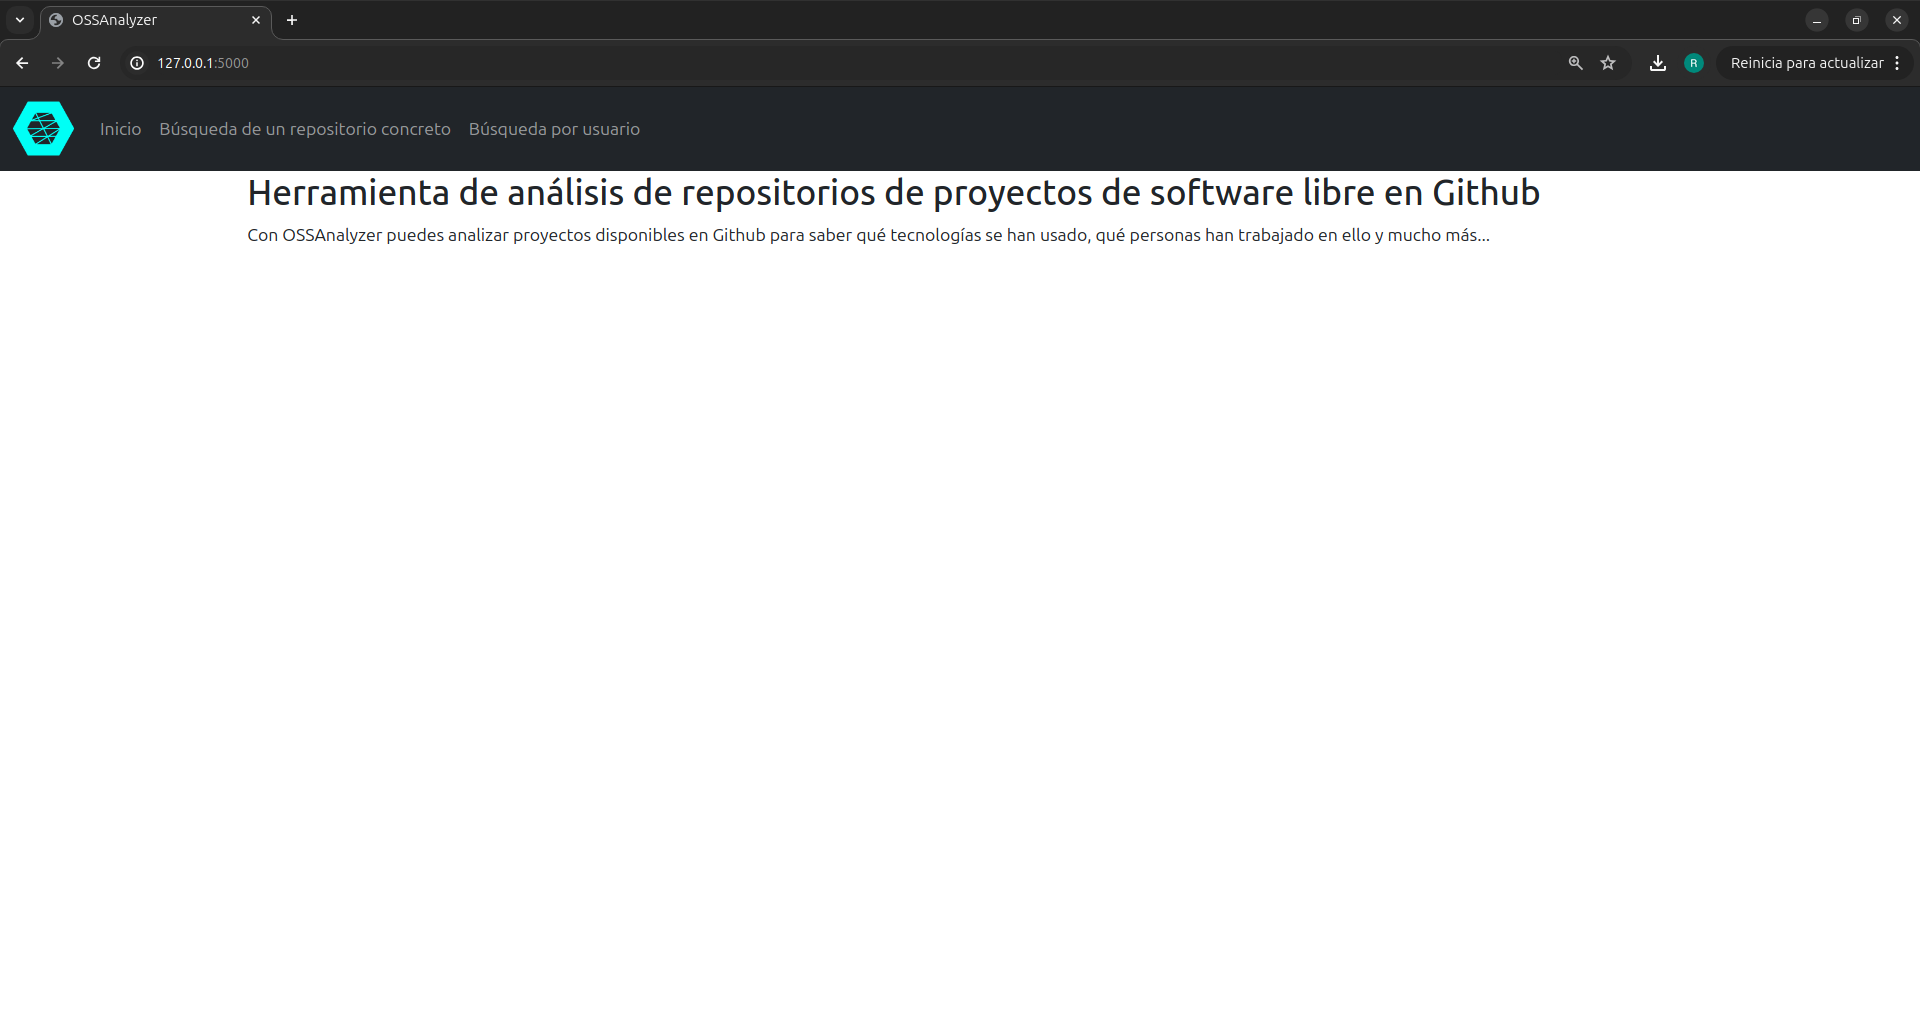
\includegraphics[width=1\textwidth]{img/paginaprincipal.png}
  \caption{Página principal de la aplicación}
  \label{figura:mainpage2}
\end{figure}

Tras ello aparece el formulario donde deberemos indicar el nombre de usuario de github que es propietario de los distintos repositorios que vamos a analizar. En nuestro caso de prueba, netflix.

\begin{figure}[H]
  \centering
  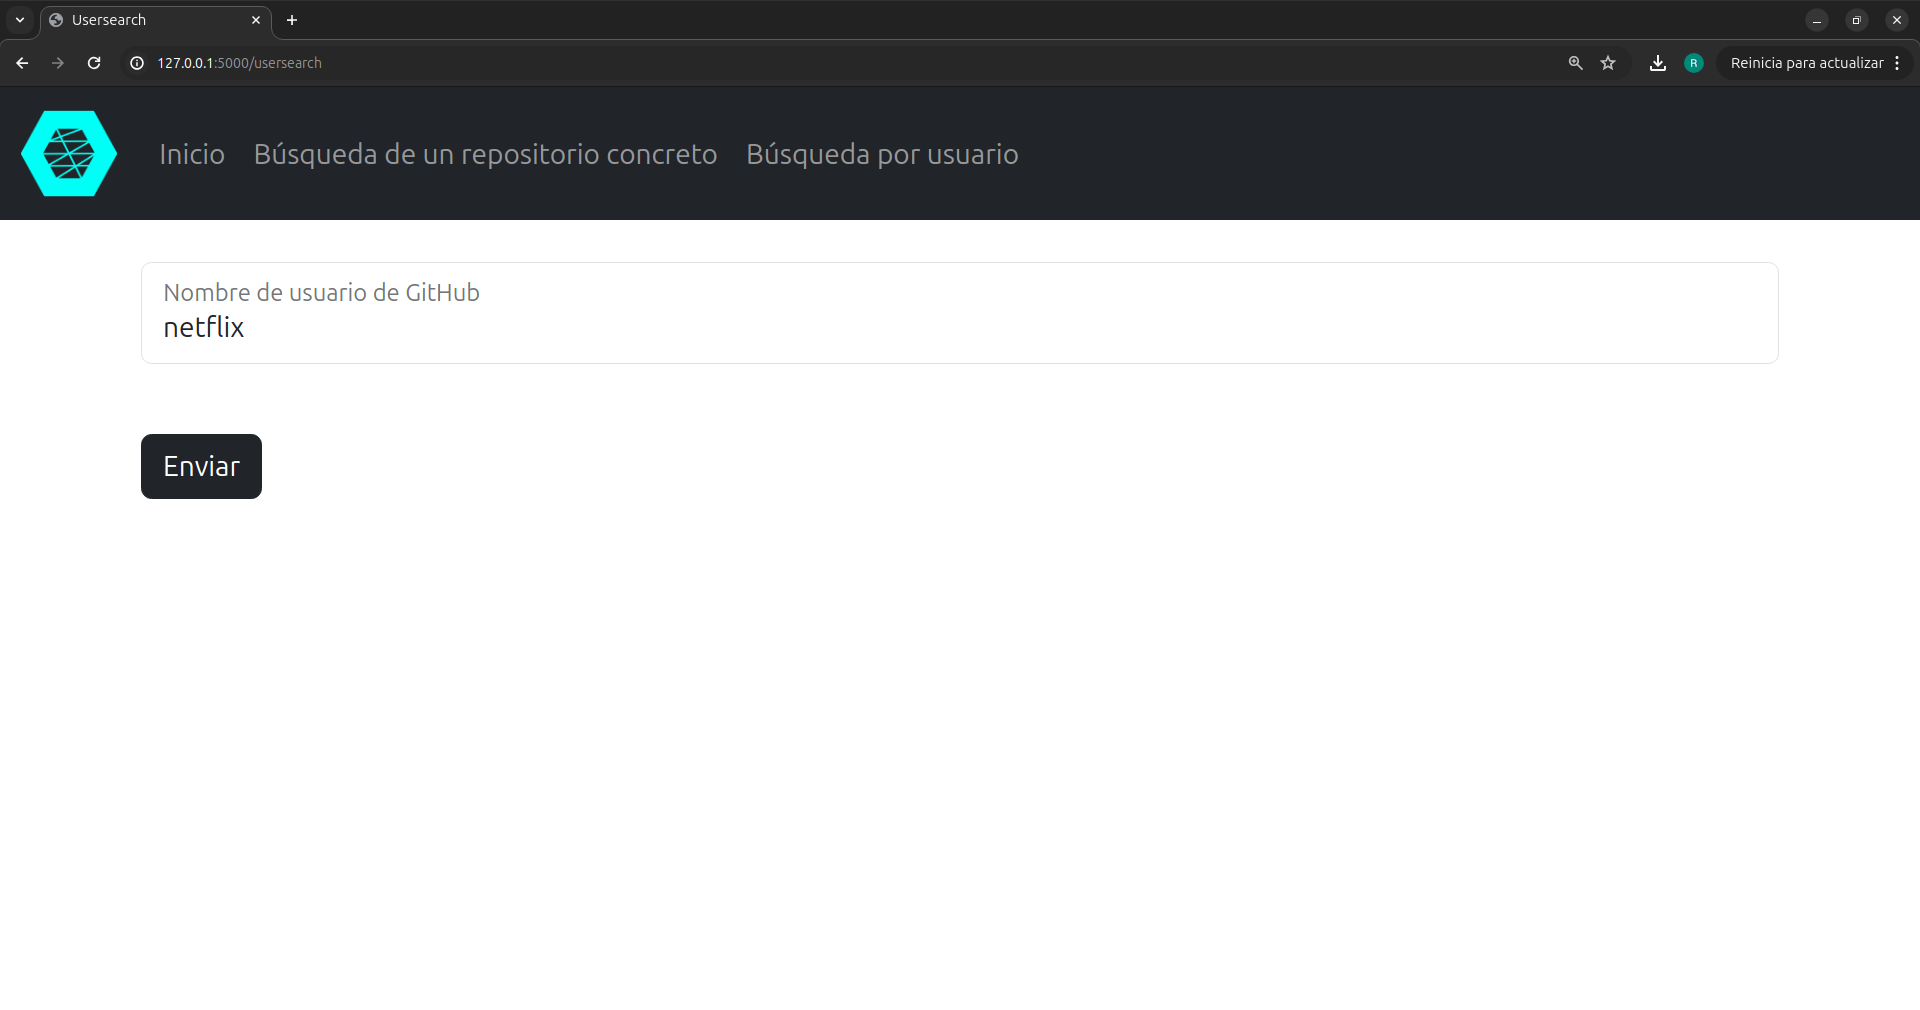
\includegraphics[width=1\textwidth]{img/getusersearch.png}
  \caption{Página que se muestra al clickar en "Búsqueda por usuario"}
  \label{figura:getusersearch}
\end{figure}

Después de pulsar el botón de envío, se envía una petición POST al endpoint /usersearch cuyo cuerpo lleva el parámetro username, con valor netflix. El servidor procesa la petición y realiza la lógica para buscar los repositorios del usuario netflix y mostrarlos en la página. Se muestra de la siguiente manera:

\begin{figure}[H]
  \centering
  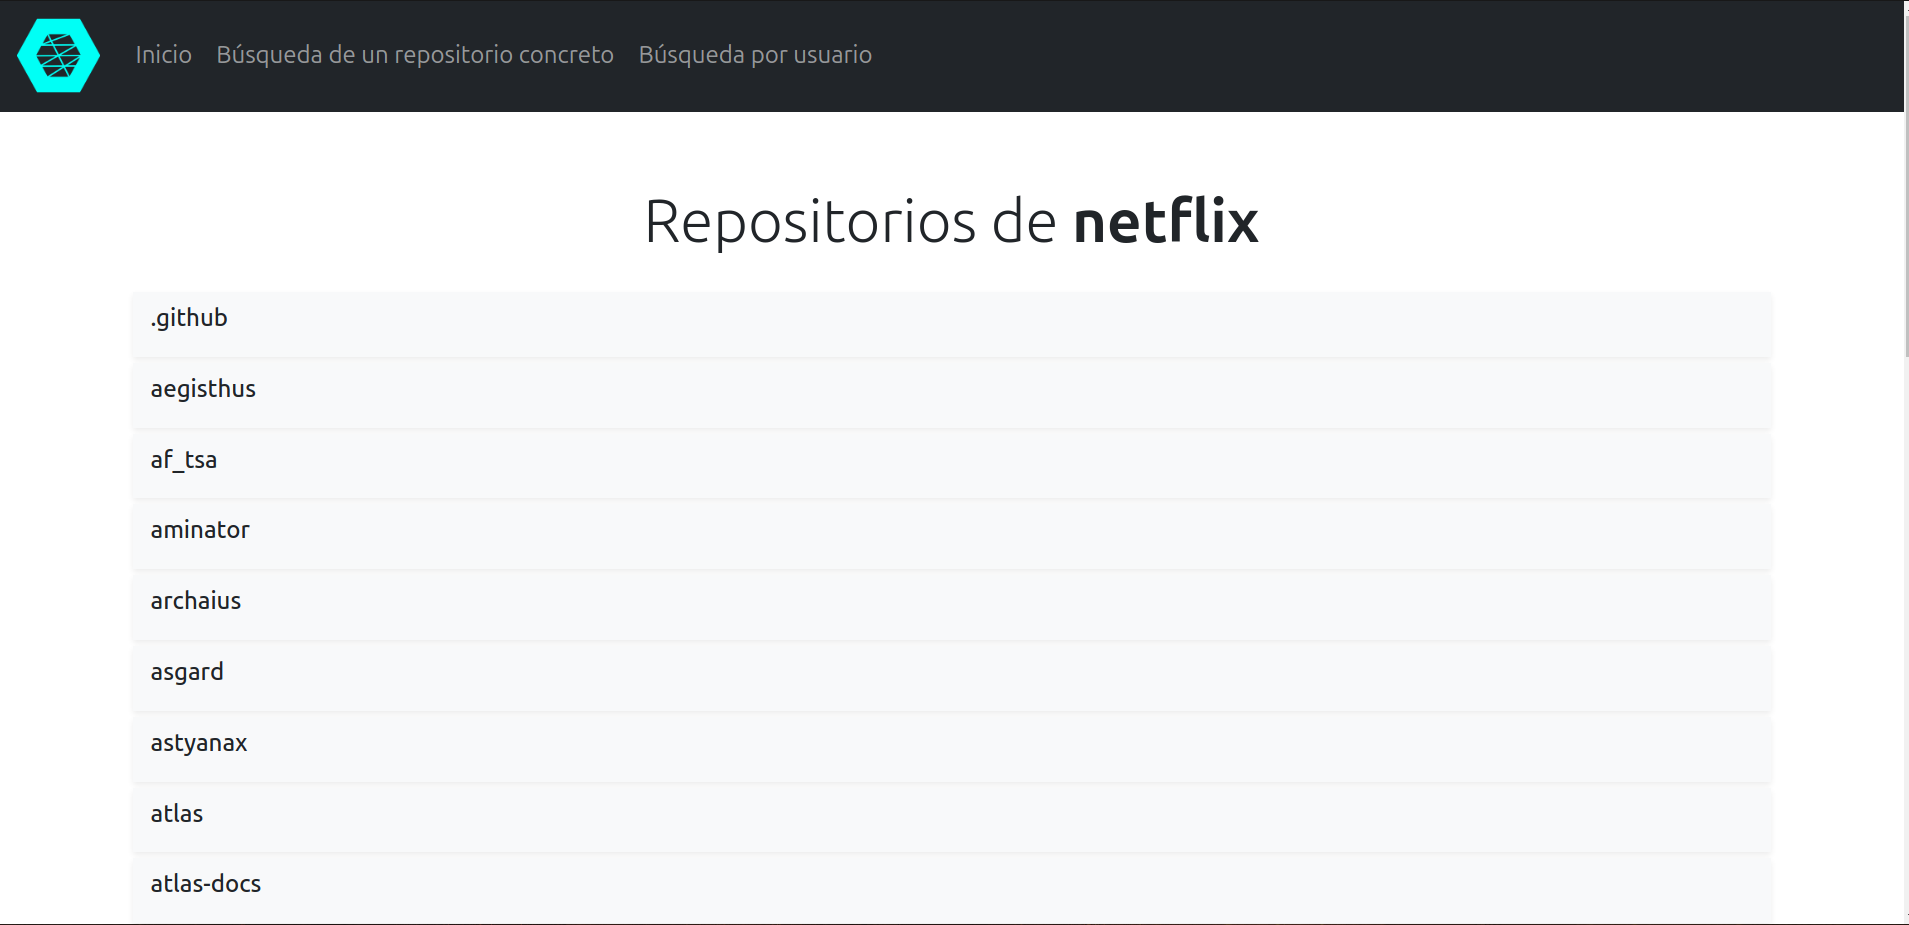
\includegraphics[width=1\textwidth]{img/listanetflix.png}
  \caption{Respuesta de la aplicación al buscar los repositorios del usuario netflix}
  \label{figura:netflixresp}
\end{figure}

Para realizar el análisis, usaremos su repositorio más popular, cuyo nombre es Hystrix. Lo encontramos entre los repositorios de la lista que hemos obtenido.


\begin{figure}[H]
  \centering
  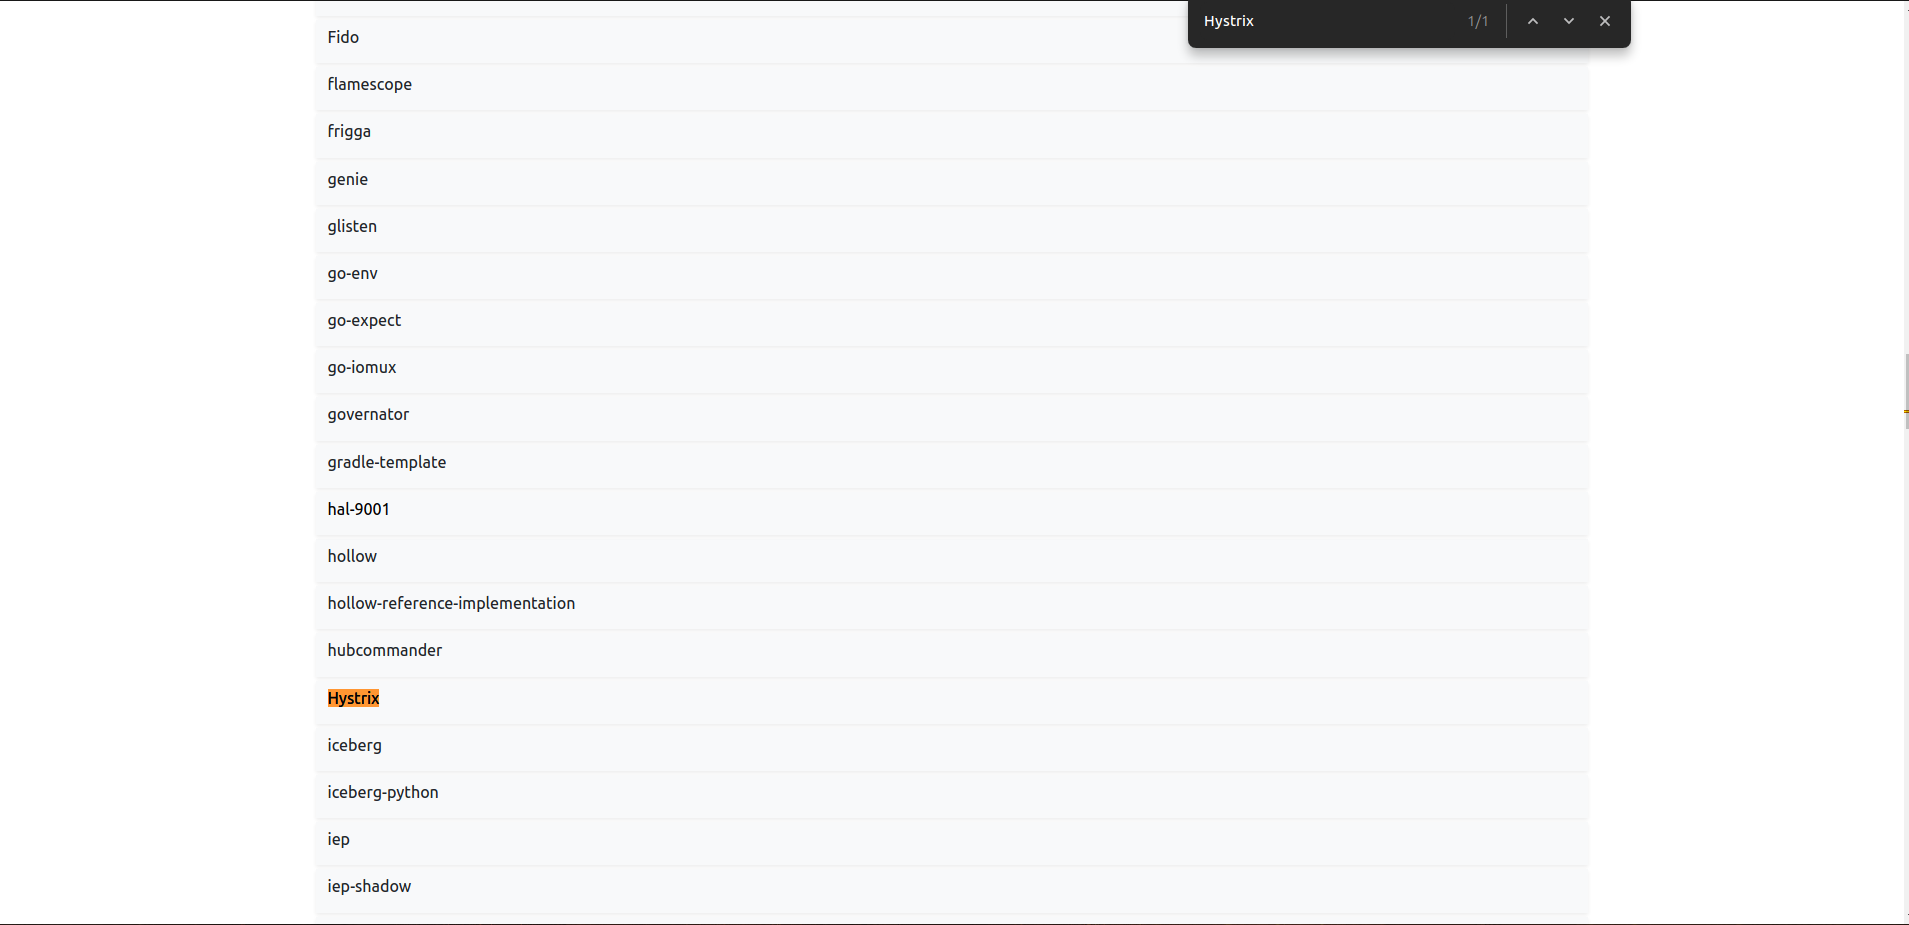
\includegraphics[width=1\textwidth]{img/hystrixenlista.png}
  \caption{Repositorio Hystrix en la lista}
  \label{figura:hystrixlist}
\end{figure}

Al hacer click, se realizará una petición POST al endpoint /userrepo, con lo que el servidor comienza el análisis del repositorio. El análisis comienza con la obtención de datos de los commits del repositorio usando la librería Perceval. El el fichero de logs, se registra que se han cogido 2354 commits realizados:

\begin{figure}[H]
  \centering
  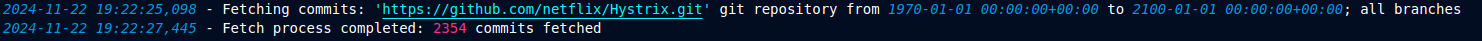
\includegraphics[width=1\textwidth]{img/logperceval.png}
  \caption{Log que se genera cuando Perceval obtiene la información de un repositorio}
  \label{figura:logperceval}
\end{figure}

Sobre estos datos, después de hacer el parseo correspondiente y las modificaciones necesarias, se obtiene un diccionario con los datos de cada uno de los usuarios que ha contribuido, los lenguajes sobre los que ha hecho esos commits, y la cantidad de los mismos.

Después, se almacenan los datos en la tabla Repository para almacenar ese repositorio, ya que suponiendo que no se ha analizado anteriormente el repositorio Hystrix del usuario netflix, se debe guardar en la base de datos. Se almacena de la siguiente manera:

\begin{figure}[H]
  \centering
  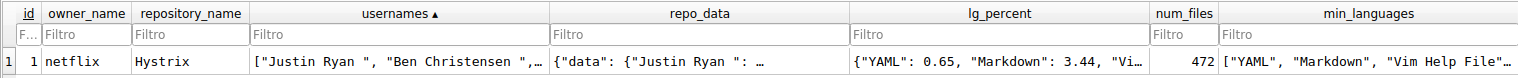
\includegraphics[width=1\textwidth]{img/HYSTRIXBBDD1.png}
  \caption{Repositorio Hystrix en la tabla Repository}
  \label{figura:hystrixbbdd}
\end{figure}

\begin{figure}[H]
  \centering
  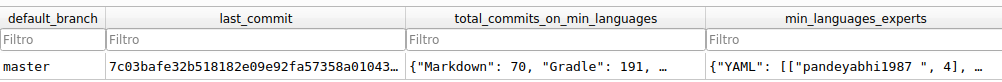
\includegraphics[width=1\textwidth]{img/HYSTRIXBBDD2.png}
  \caption{Repositorio Hystrix en la tabla Repository - 2} 
  \label{figura:hystrixbbdd2}
\end{figure}


Además, para nuestro análisis personal final, guardaremos los datos de cada uno de los usuarios que ha participado en este repositorio, junto a las modificaciones sobre cada uno de los lenguajes y la lista de repositorios que hemos analizado en los que ha contribuido (Al ser este el primero que analizamos, solo tendrán en la lista este repositorio). Se almacenan así:

\begin{figure}[H]
  \centering
  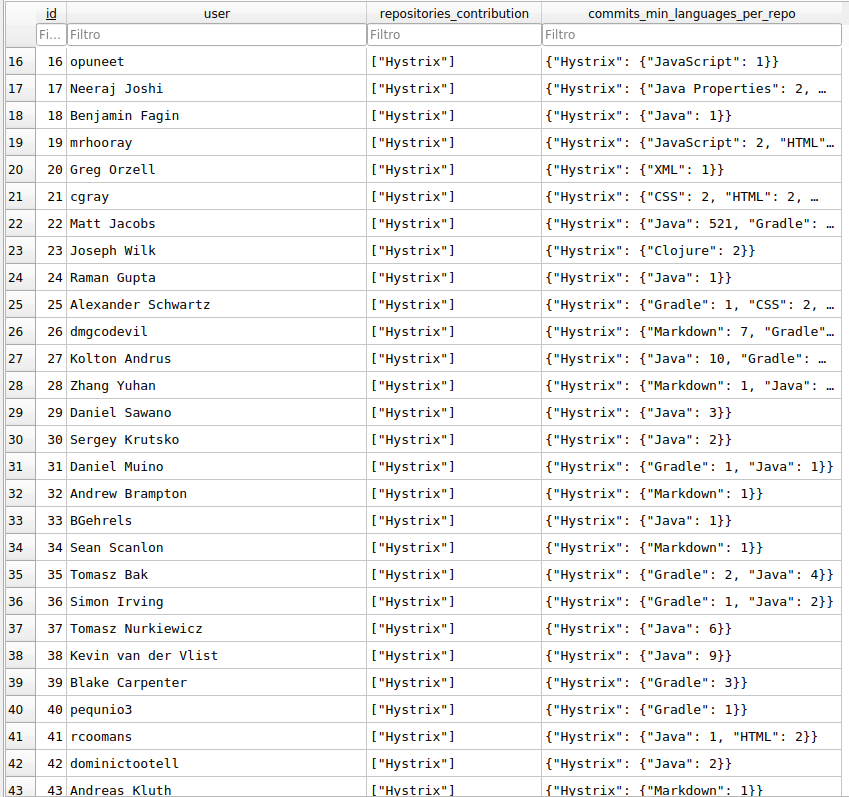
\includegraphics[width=1\textwidth]{img/hystrixuserexpertise.png}
  \caption{Repositorio Hystrix en la tabla User\_expertise}
  \label{figura:hystrixuserexpertise}
\end{figure}

Por último, se almacena en la tabla Languages cada uno de los lenguajes que forman el repositorio, la lista de usuarios de que ha realizado commits sobre ese lenguaje, el número total de usuarios que lo ha usado, y el número total de commits sobre el mismo. Queda así:

\begin{figure}[H]
  \centering
  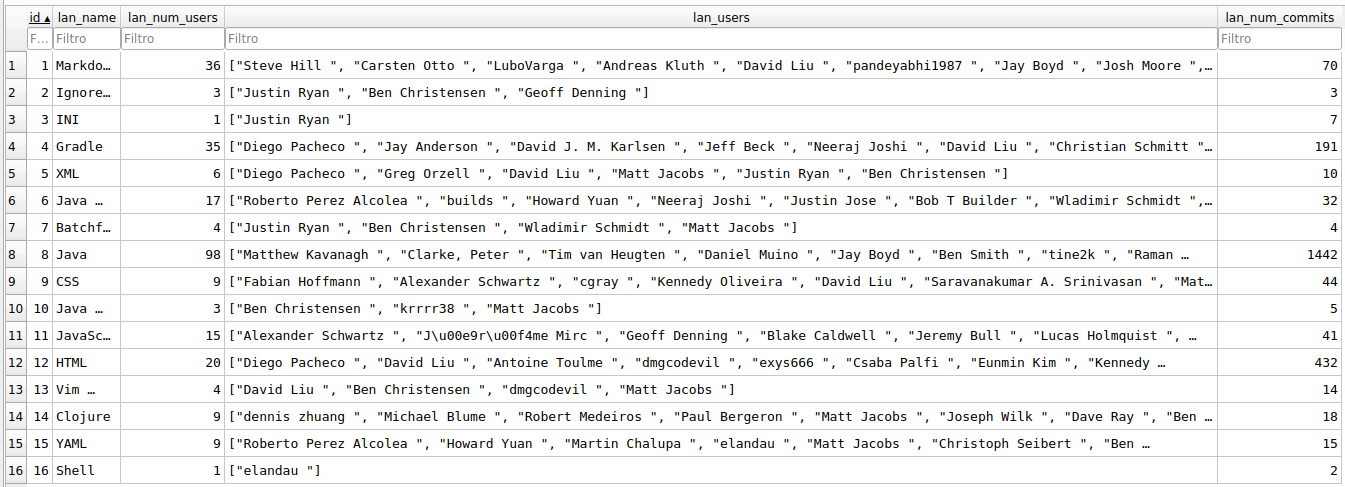
\includegraphics[width=1\textwidth]{img/hystrixlanguages.png}
  \caption{Repositorio Hystrix en la tabla Languages}
  \label{figura:hystrixlanguages}
\end{figure}

Ahora que se ha hecho la recolección y almacenaje de los datos, queda la representación gráfica para que el usuario que ha querido analizar el repositorio, pueda verlo de manera sencilla.

\begin{figure}[H]
  \centering
  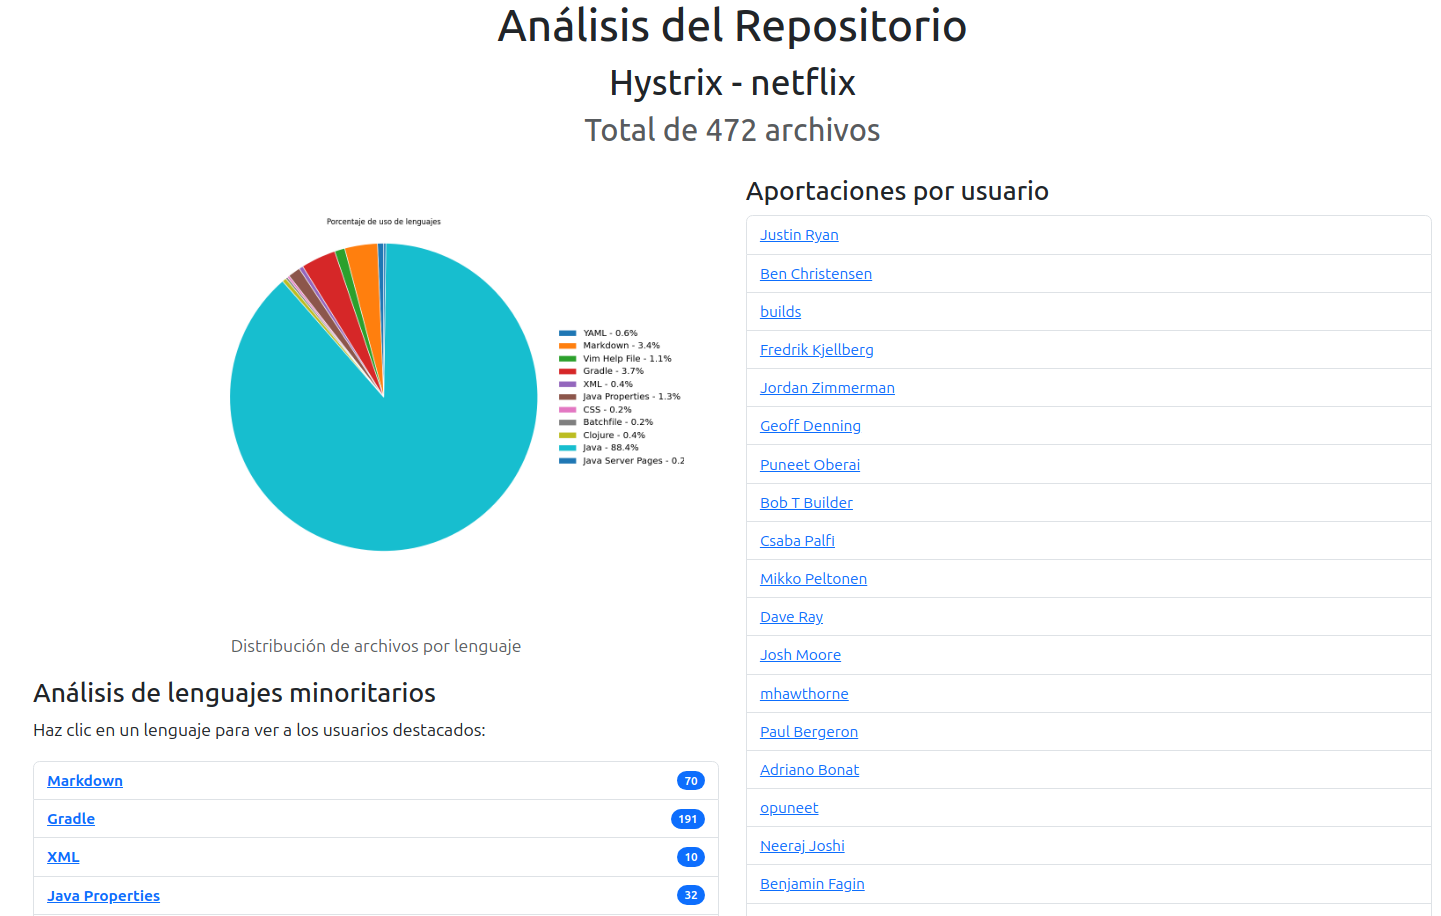
\includegraphics[width=1\textwidth]{img/analisishystrix.png}
  \caption{Representación gráfica del análisis del repositorio Hystrix - 1}
  \label{figura:analisishystrix1}
\end{figure}

\begin{figure}[H]
  \centering
  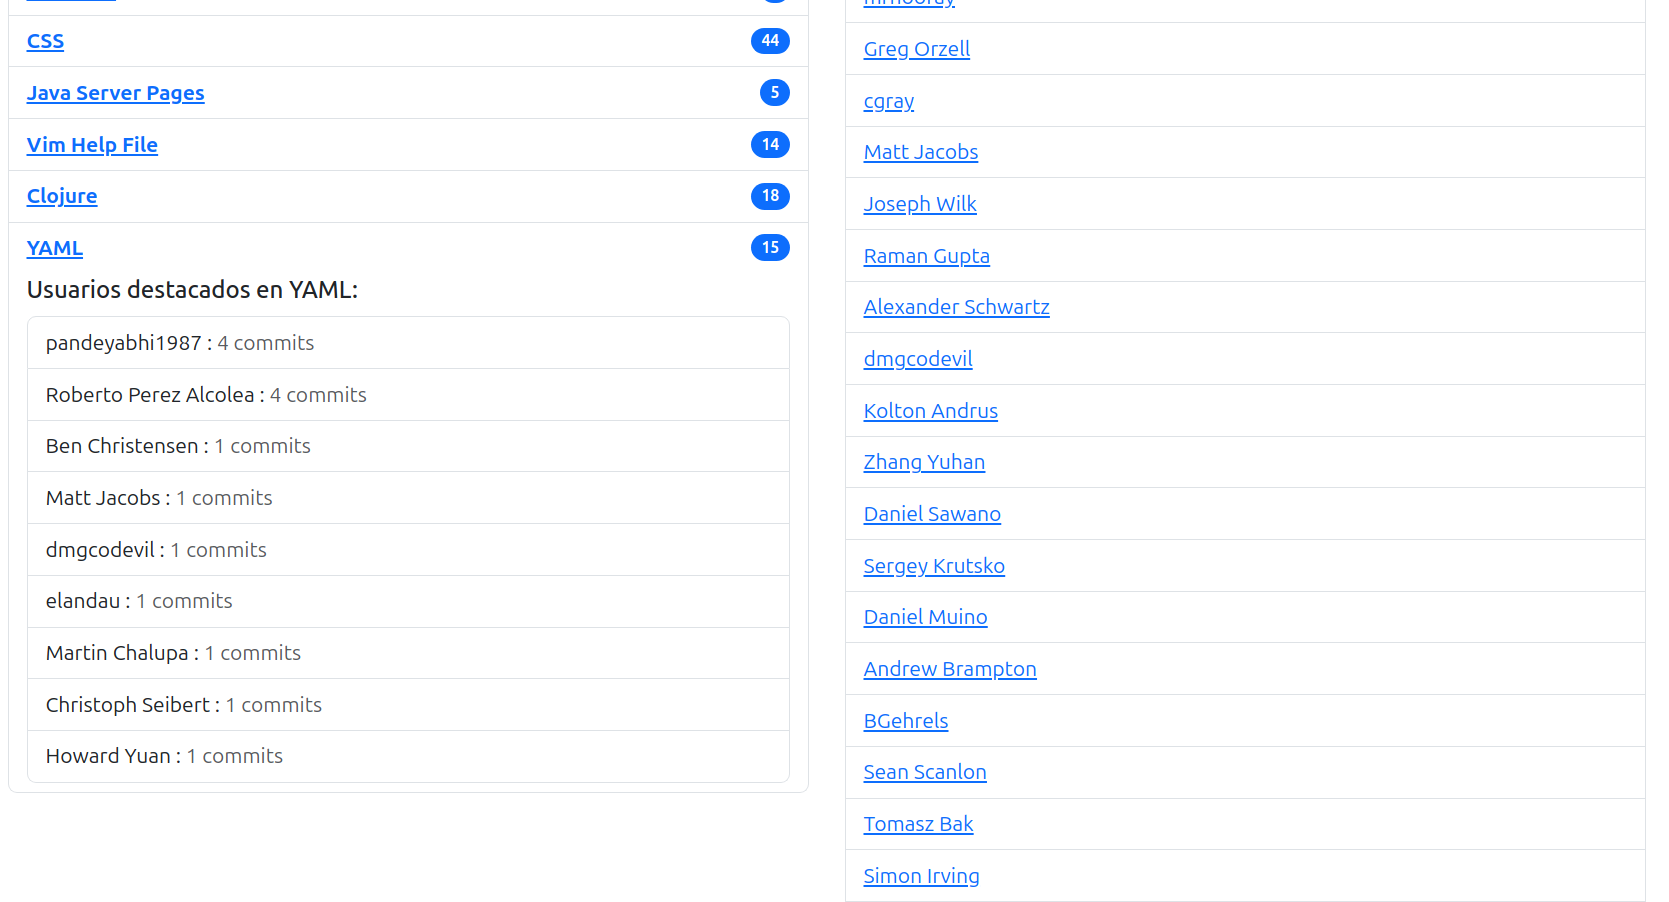
\includegraphics[width=1\textwidth]{img/analisishystrix2.png}
  \caption{Representación gráfica del análisis del repositorio Hystrix - 2}
  \label{figura:analisishystrix2}
\end{figure}

\begin{figure}[H]
  \centering
  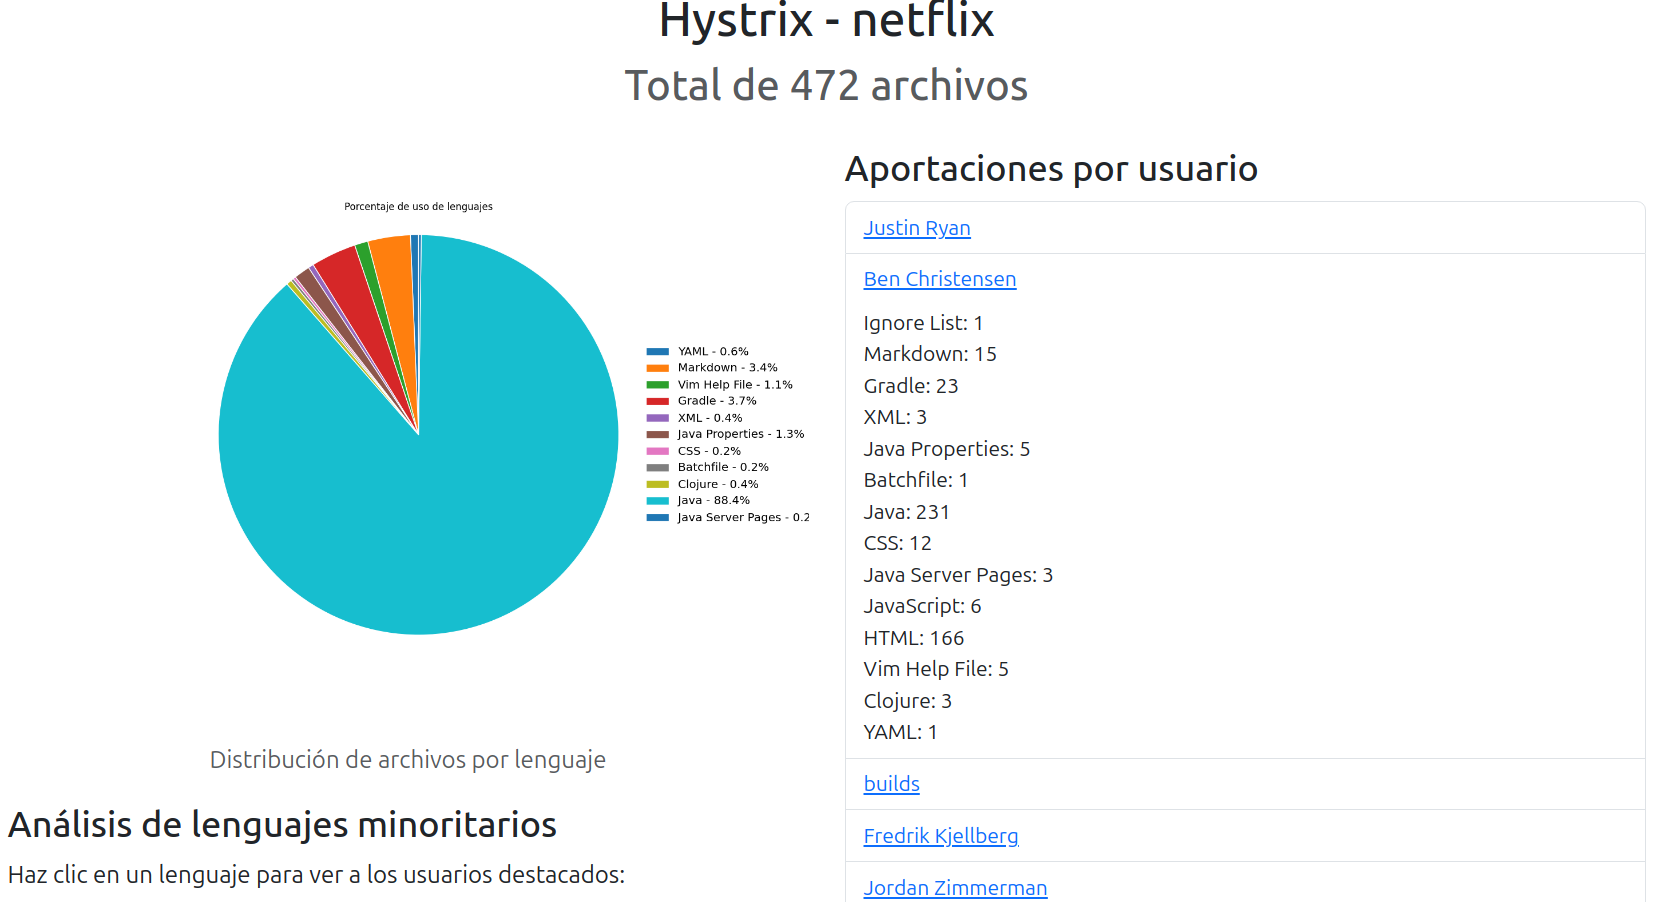
\includegraphics[width=1\textwidth]{img/analisishystrix3.png}
  \caption{Representación gráfica del análisis del repositorio Hystrix - 3}
  \label{figura:analisishystrix3}
\end{figure}

En las figuras 5.10, 5.11 y 5.12 se muestra el resultado del análisis. En este repositorio hay 472 ficheros en total, y hay 11 lenguajes. El lenguaje mayoritario es Java, con un 88,4\% de ocupación. Los lenguajes minoritarios son YAML, Markdown, VIM Help File (TXT), Gradle, XML, Java Properties, CSS, Batchfile, Clojure y Java Server Page, que representan menos del 5\%. Se muestra la información acerca de las contribuciones al repositorio en estos lenguajes minoritarios de parte de  cada uno de los usuarios, y la lista de todos los usuarios con su participación en el repositorio.

\section{Análisis de más repositorios}
\label{sec:Análisis de más repositorios}

Para ver el análisis en más repositorios del usuario netflix, he escogido 9 repositorios. Muestro el análisis realizado de todos ellos.

\begin{figure}[H]
  \centering
  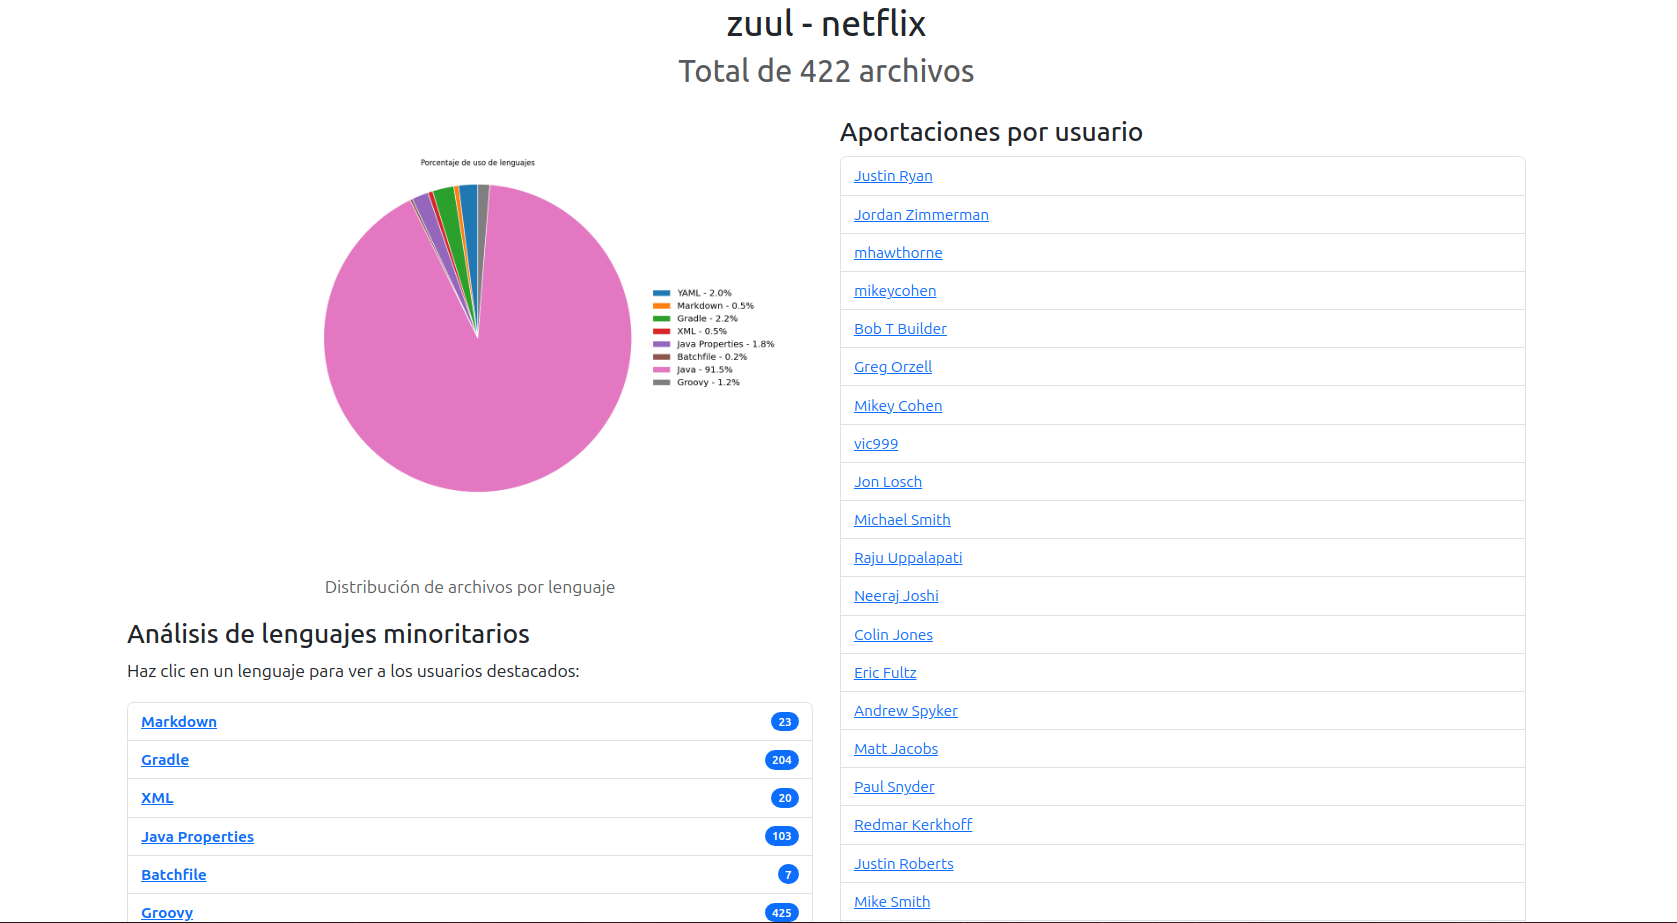
\includegraphics[width=1\textwidth]{img/zuul.png}
  \caption{Representación gráfica del análisis del repositorio Zuul}
  \label{figura:analisiszuul}
\end{figure}

En el repositorio Zuul, el lenguaje mayoritario es Java con un 91,5\%, mientras que YAML, Markdown, Gradle, XML, Java Properties, Batchfile y Groovy son lenguajes minoritarios. Se muestran las contribuciones de cada usuario a cada uno de los lenguajes minoritarios y la lista de todos los usuarios que han participado en el proyecto.

\begin{figure}[H]
  \centering
  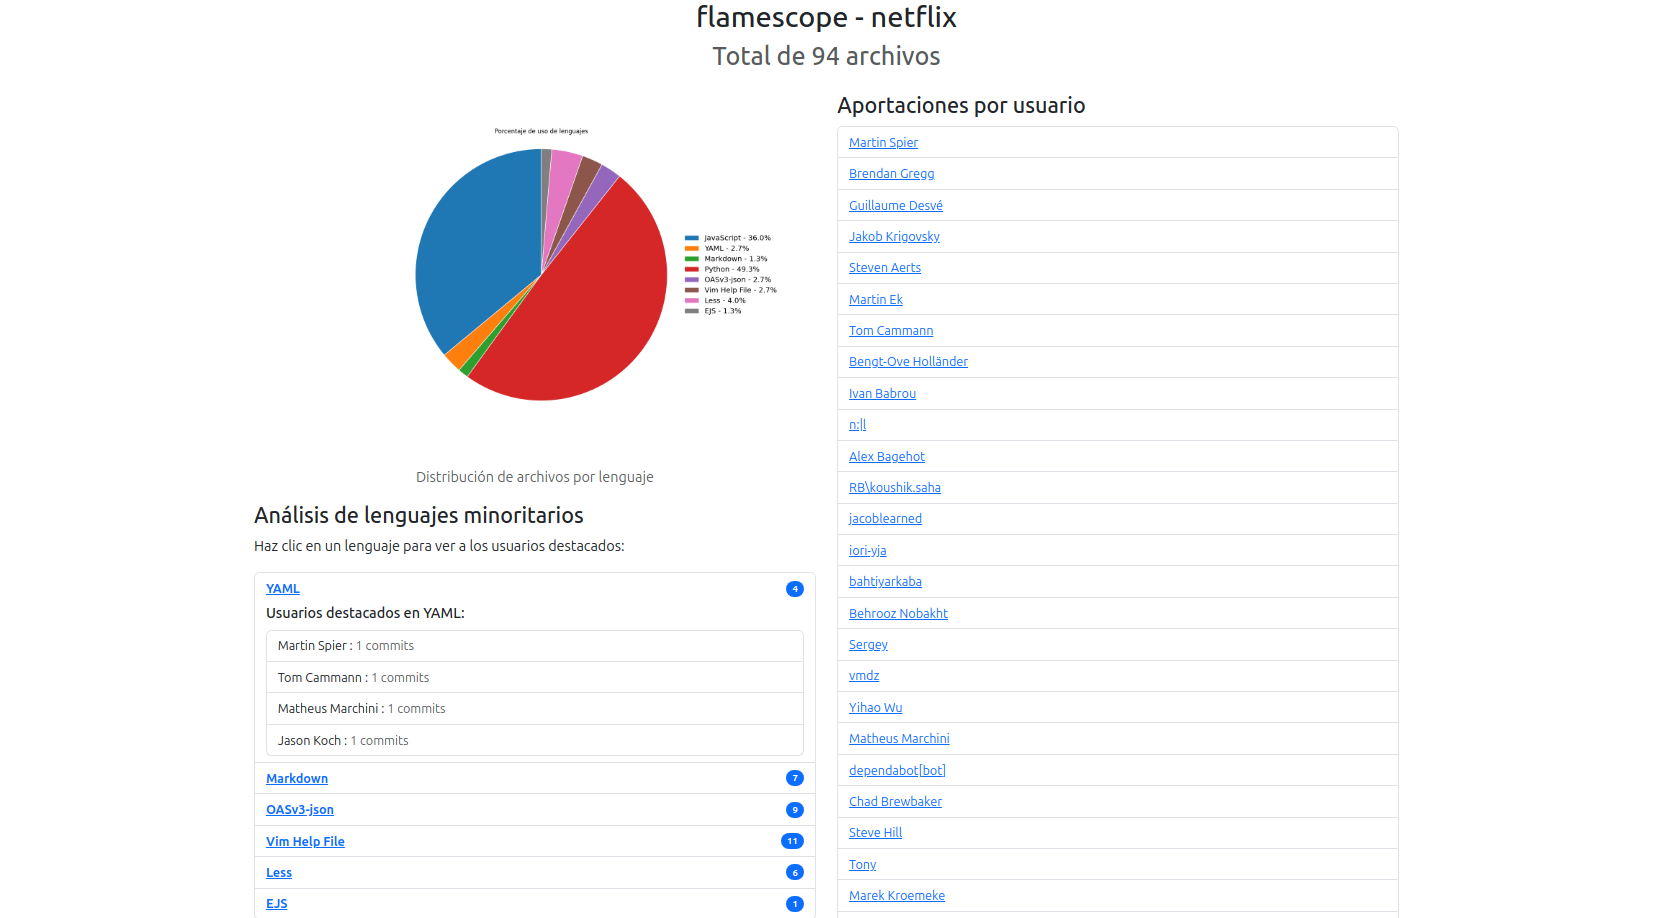
\includegraphics[width=1\textwidth]{img/flamescope.png}
  \caption{Representación gráfica del análisis del repositorio Flamescope}
  \label{figura:analisisflamescope}
\end{figure}

En el repositorio Flamescope los lenguajes mayoritarios se reparten más, y en este caso no es Java el lenguaje principal, sino Python, con un 49,3\% de ocupación. Le sigue JavaScript con un 36,0\%, que también es mayoritario. El resto, YAML, Markdown, JSON, VIM Help File (TXT), Less y EJS son los lenguajes minoritarios.

\begin{figure}[H]
  \centering
  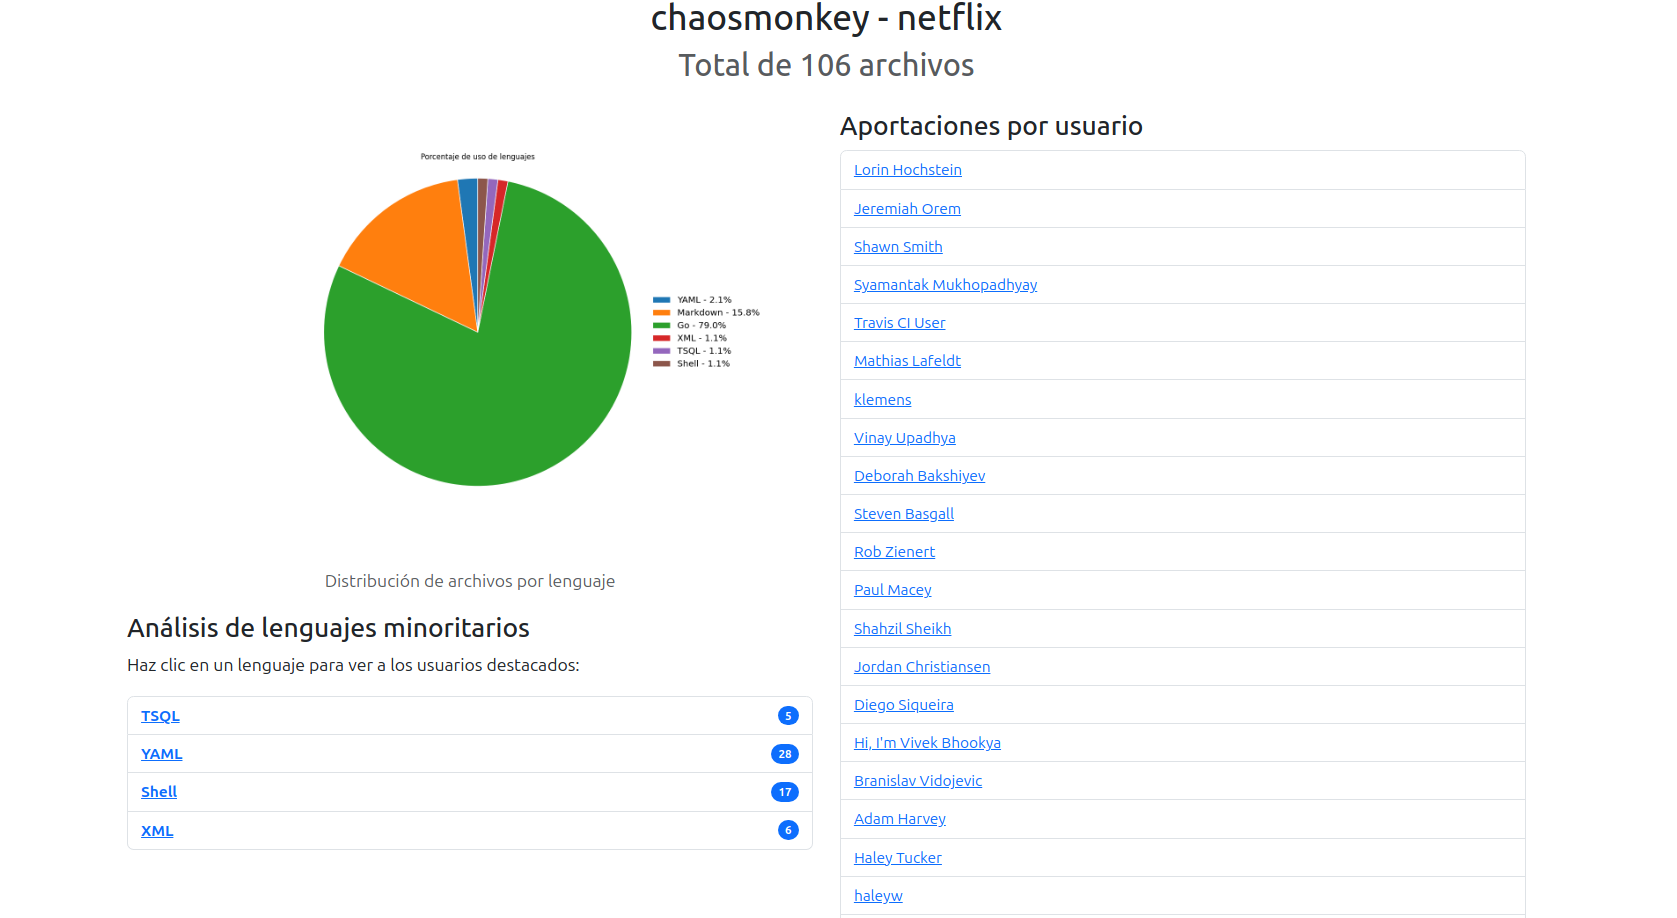
\includegraphics[width=1\textwidth]{img/chaosmonkey.png}
  \caption{Representación gráfica del análisis del repositorio chaosmonkey}
  \label{figura:analisischaosmonkey}
\end{figure}

En esta ocasión, en el repositorio chaosmonkey, los dos lenguajes mayoritarios son Go con un 79\% y Markdown con un 15,8\%. YAML, XML, TSQL y Shell son minoritarios.

\begin{figure}[H]
  \centering
  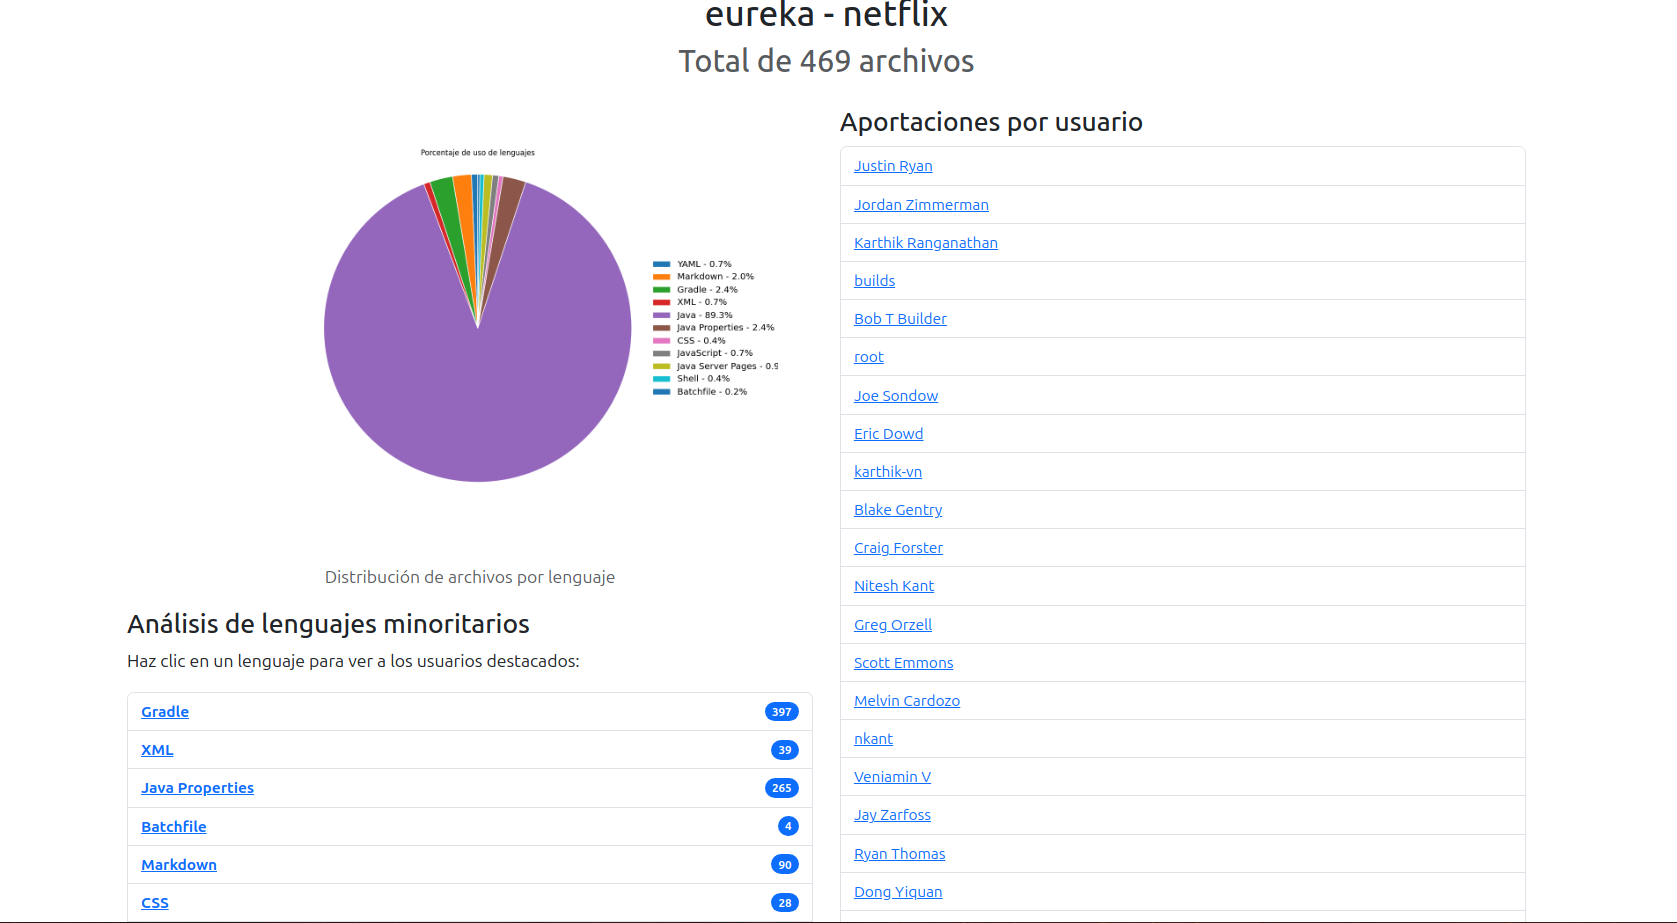
\includegraphics[width=1\textwidth]{img/eureka.png}
  \caption{Representación gráfica del análisis del repositorio Eureka}
  \label{figura:analisiseureka}
\end{figure}

Del repositorio eureka, Java es el lenguaje principal con un 89,3\% de uso total, mientras que el resto de lenguajes que se han usado en el repositorio son todos minoritarios. Es un repositorio bastante grande, con 469 ficheros totales y un gran número de commits en algunos lenguajes minoritarios como Gradle o Java Properties.
\begin{figure}[H]
  \centering
  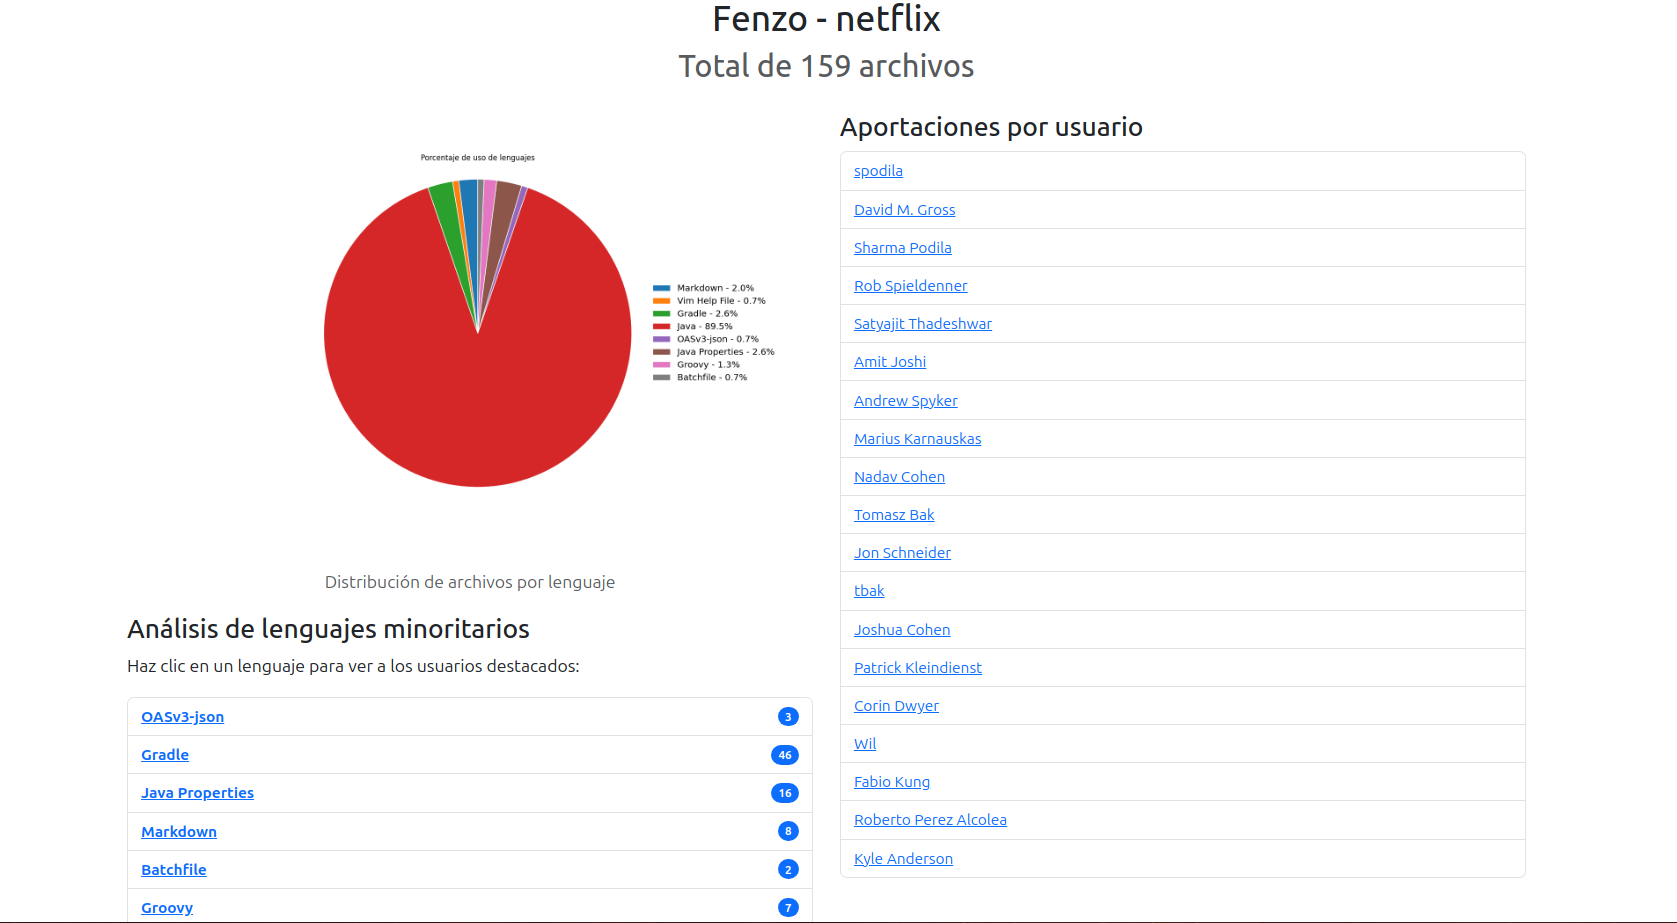
\includegraphics[width=1\textwidth]{img/fenzo.png}
  \caption{Representación gráfica del análisis del repositorio Fenzo}
  \label{figura:analisisfenzo}
\end{figure}

En el repositorio Fenzo, los lenguajes minoritarios son Markdown, VIM Help File (TXT), Gradle, JSON, Java Properties, Groovy y Batchfile. En este caso, aunque haya 159 archivos, se han realizado pocos commits sobre los lenguajes minoritarios, a excepción de Gradle. Java es el único lenguaje mayoritario, con un 89,5\%.

\begin{figure}[H]
  \centering
  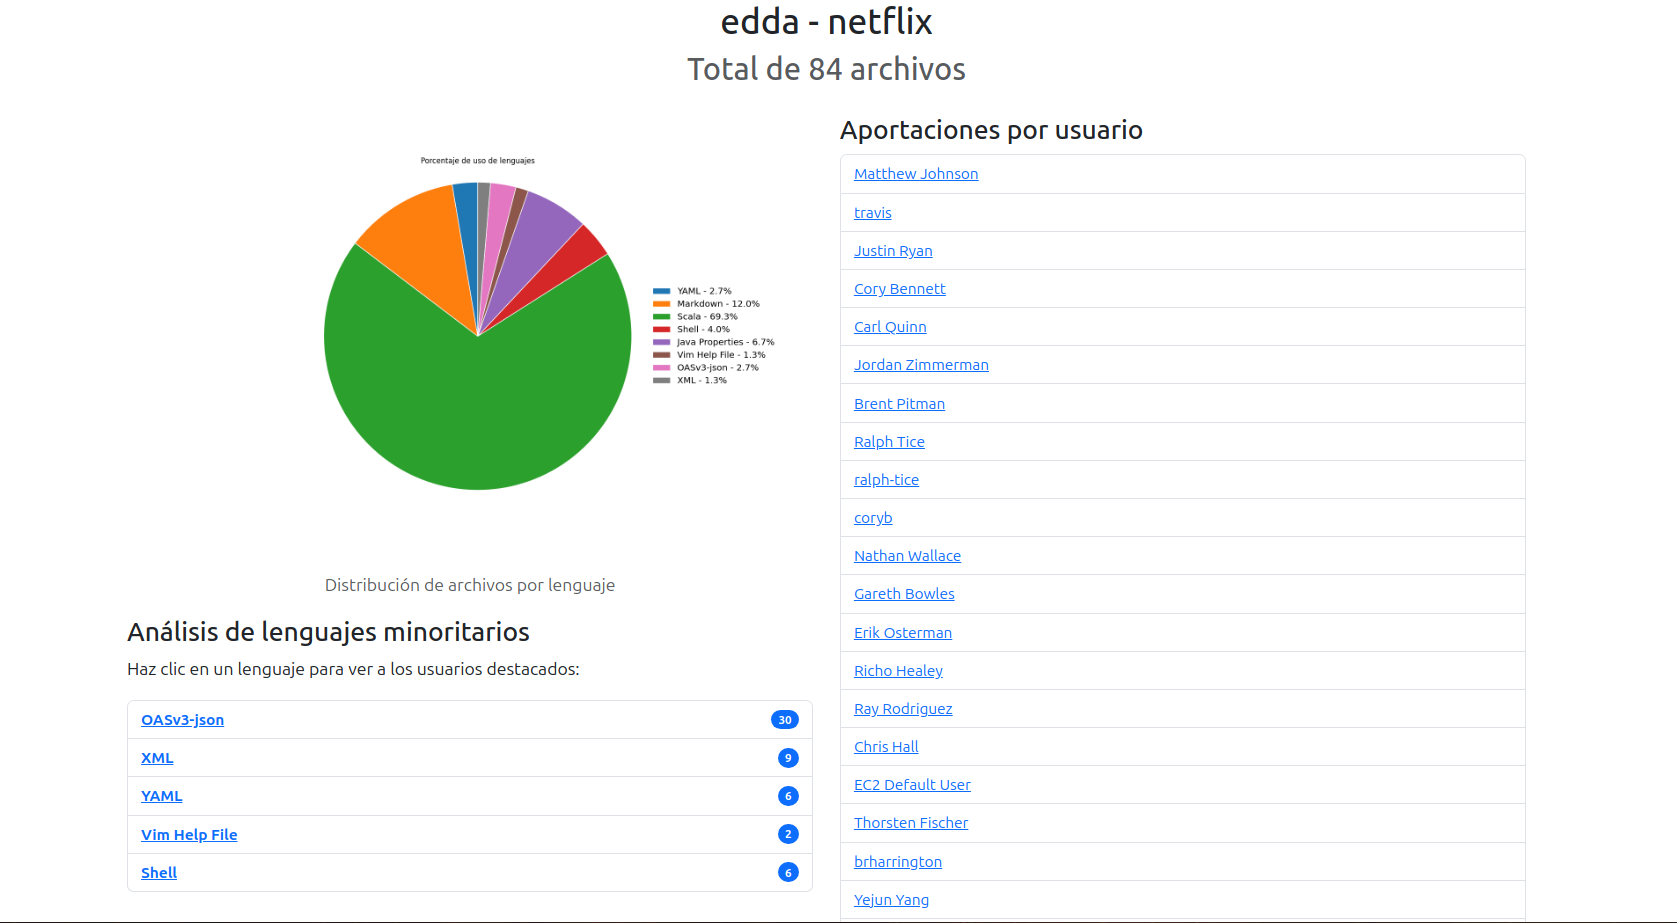
\includegraphics[width=1\textwidth]{img/edda.png}
  \caption{Representación gráfica del análisis del repositorio Edda}
  \label{figura:analisisedda}
\end{figure}

En este repositorio Scala es el lenguaje principal con un 69,3\% de uso, seguido de Markdown con un 12\%. No es un repositorio muy grande, cuenta con 84 archivos y los lenguajes minoritarios, a excepción de JSON, cuentan con pocas contribuciones.

\begin{figure}[H]
  \centering
  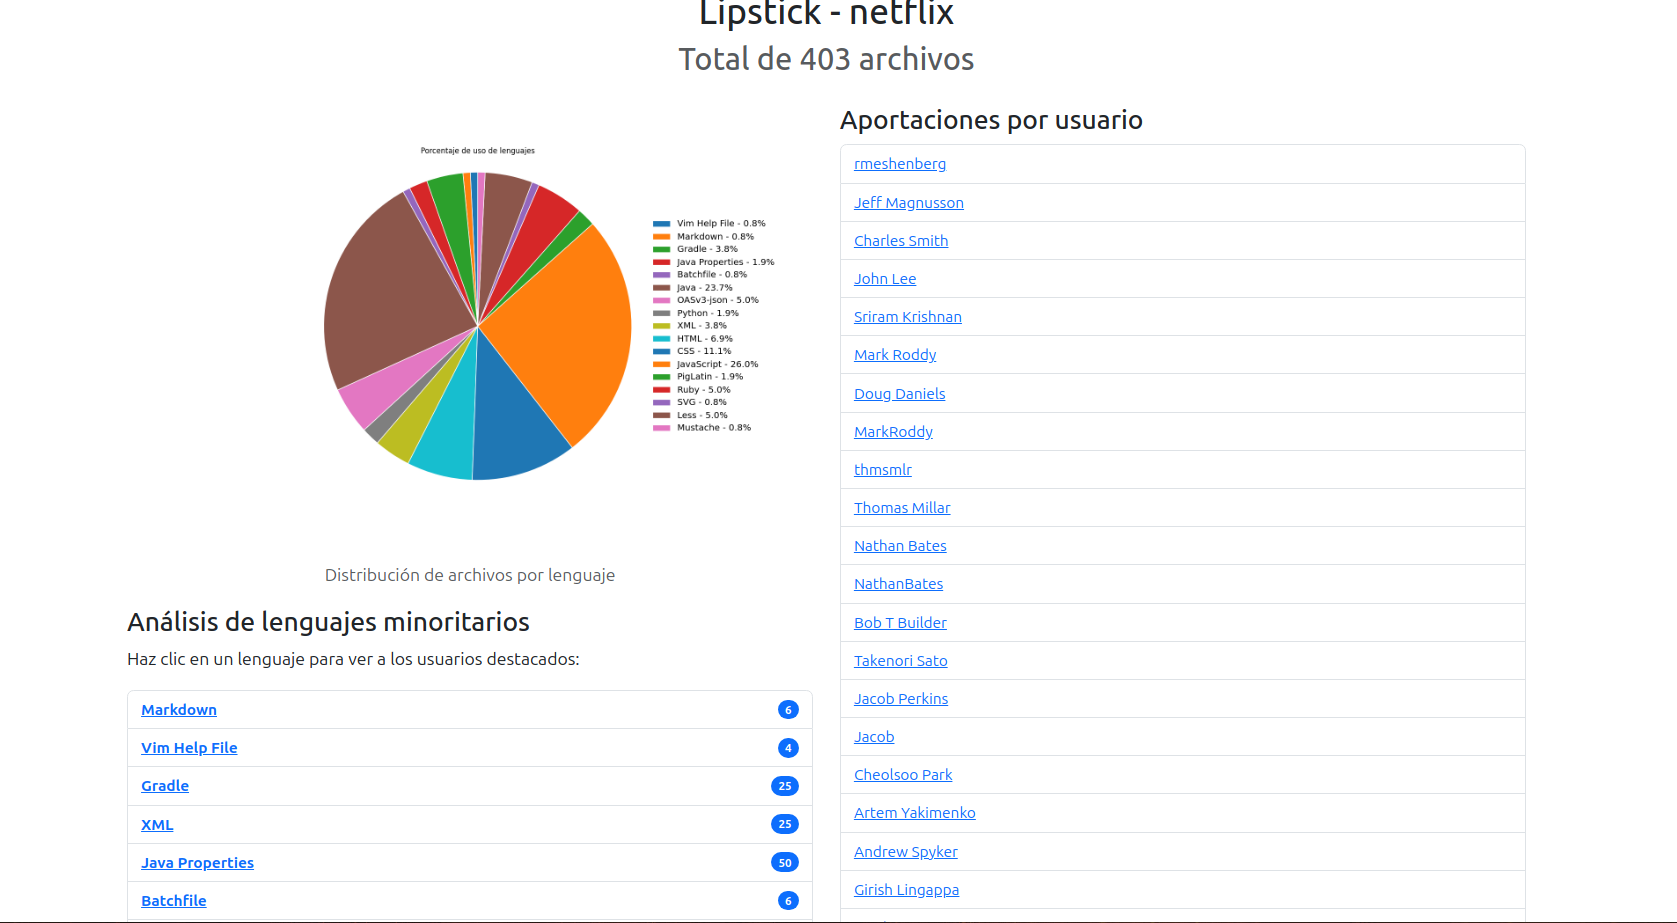
\includegraphics[width=1\textwidth]{img/lipstick.png}
  \caption{Representación gráfica del análisis del repositorio Lipstick}
  \label{figura:analisislipstick}
\end{figure}

El repositorio Lipstick tiene el uso de los lenguajes bastante repartidos y no hay un lenguaje que destaque en gran cantidad. Al estar bastante repartidos hay varios lenguajes minoritarios como Markdown o Gradle, que están siendo bastante recurrentes en los repositorios de este usuario.

\begin{figure}[H]
  \centering
  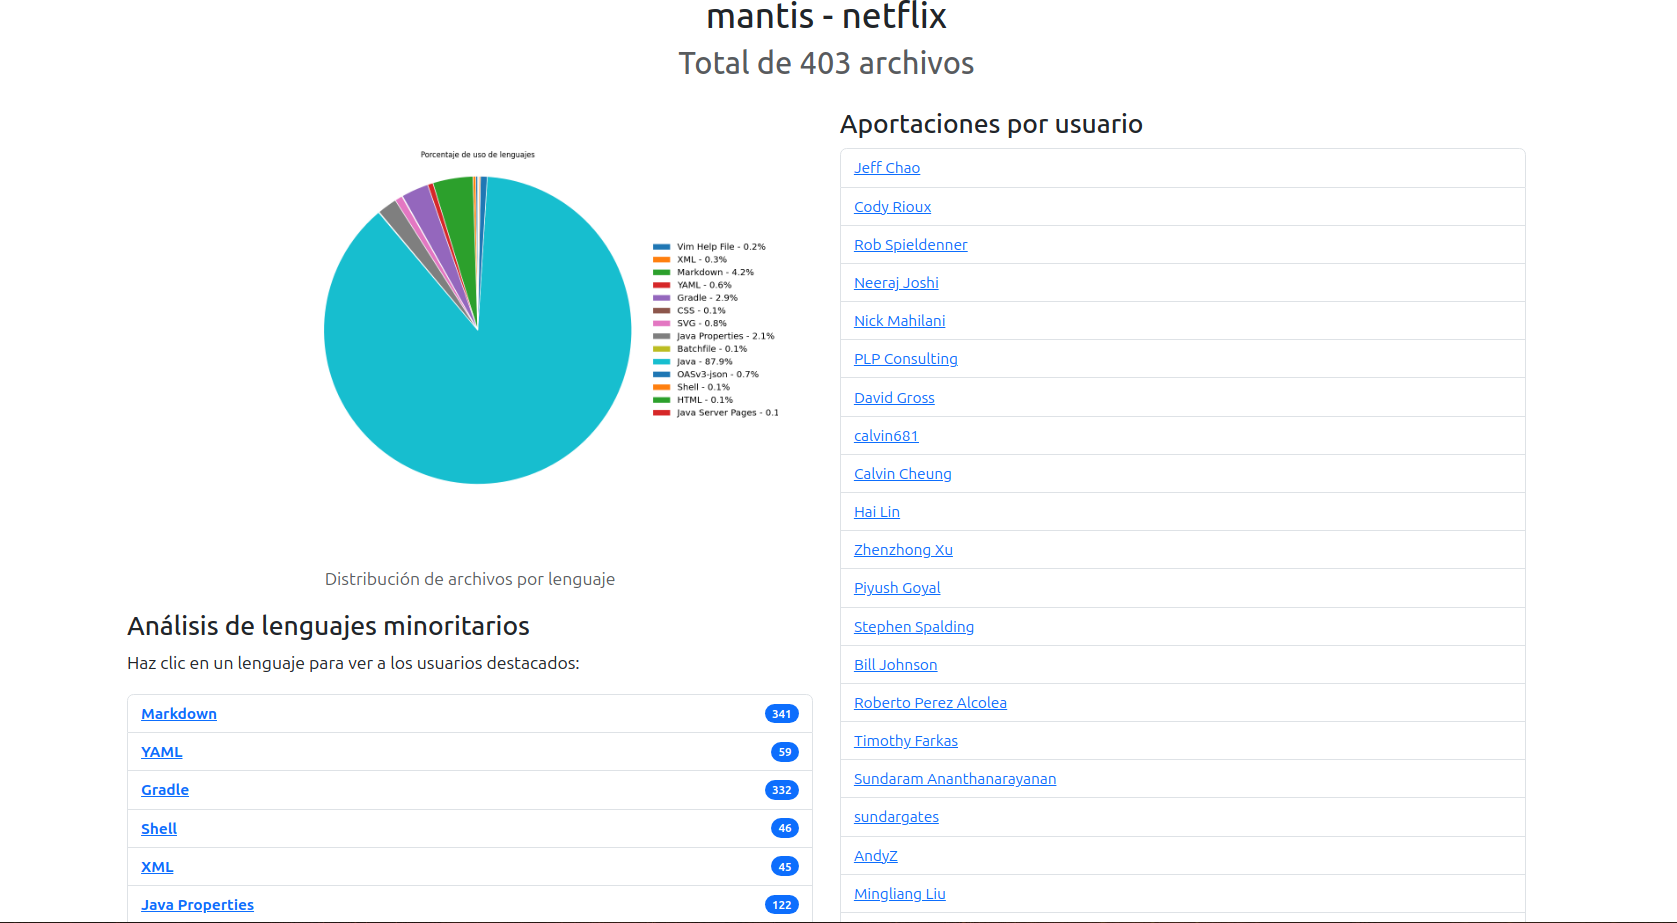
\includegraphics[width=1\textwidth]{img/mantis.png}
  \caption{Representación gráfica del análisis del repositorio Mantis}
  \label{figura:analisismantis}
\end{figure}

Este repositorio, Mantis, vuelve a tener un lenguaje mayoritario principal, Java, con un 87,9\% de ocupación entre todos los ficheros. El resto, son todos lenguajes minoritarios con bastante participación.

\begin{figure}[H]
  \centering
  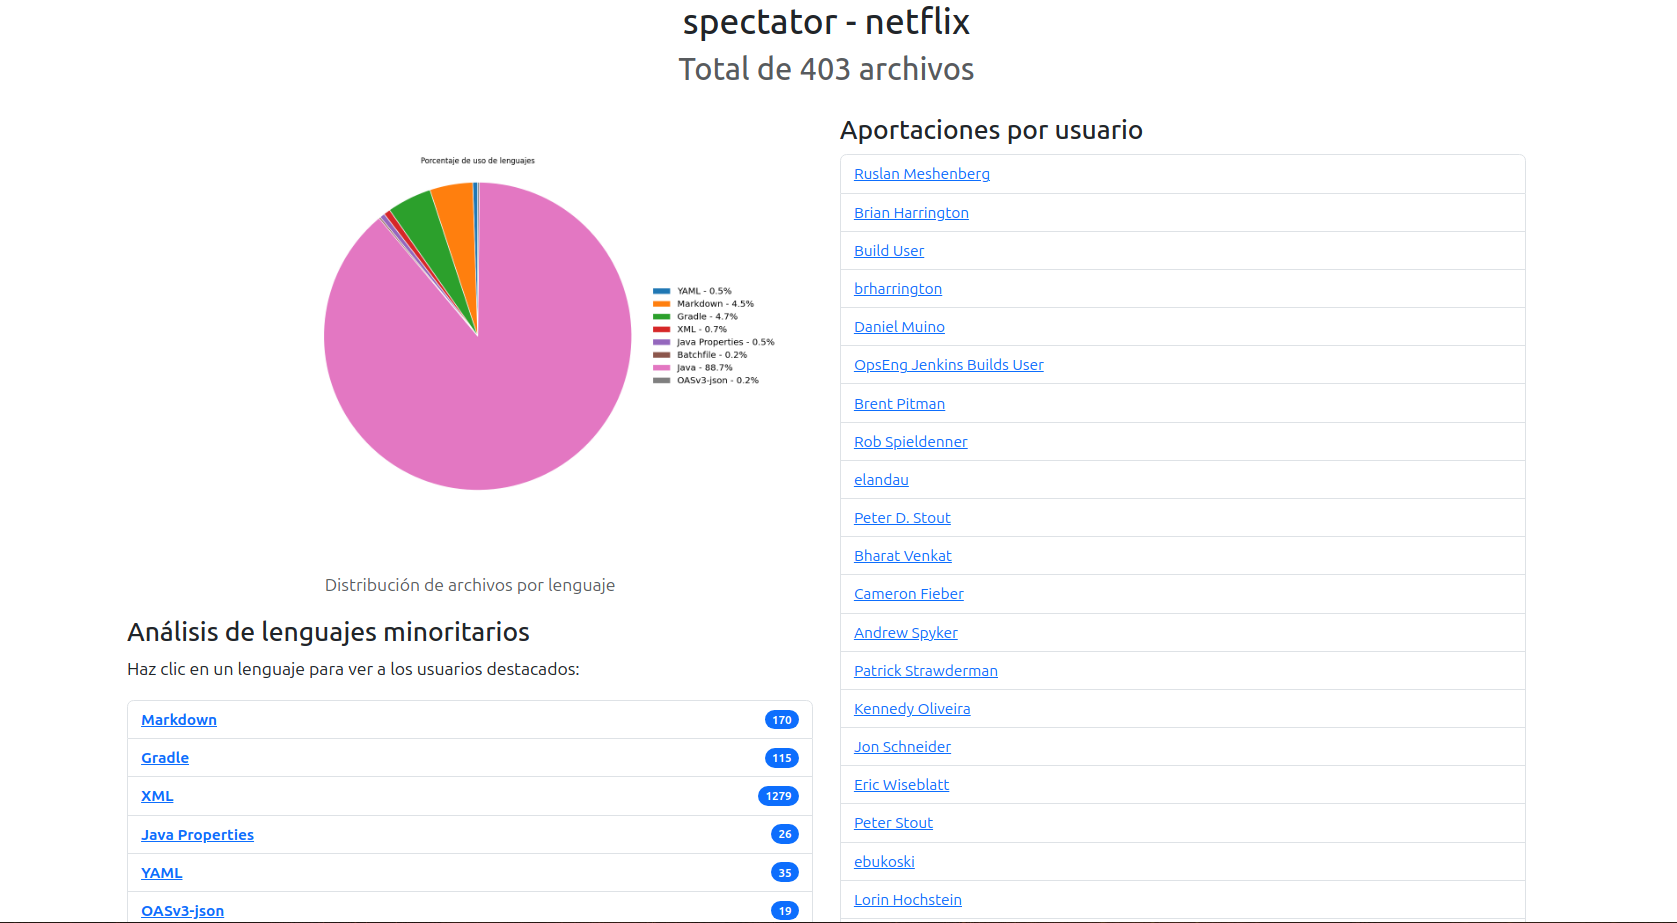
\includegraphics[width=1\textwidth]{img/spectator.png}
  \caption{Representación gráfica del análisis del repositorio spectator}
  \label{figura:analisisspectator}
\end{figure}

Spectator vuelve a ser un repositorio con Java como lenguaje principal, mientras que el resto son todos minoritarios. Destaca el número de contribuciones realizadas sobre ficheros XML con 1279 contribuciones entre todos los usuarios.

%%%%%%%%%%%%%%%%%%%%%%%%%%%%%%%%%%%%%%%%%%%%%%%%%%%%%%%%%%%%%%%%%%%%%%%%%%%%%%%%
%%%%%%%%%%%%%%%%%%%%%%%%%%%%%%%%%%%%%%%%%%%%%%%%%%%%%%%%%%%%%%%%%%%%%%%%%%%%%%%%
% RESULTADOS %
%%%%%%%%%%%%%%%%%%%%%%%%%%%%%%%%%%%%%%%%%%%%%%%%%%%%%%%%%%%%%%%%%%%%%%%%%%%%%%%%

\cleardoublepage
\chapter{Resultados}
\label{chap:resultados}

Se ha realizado el análisis de 200 repositorios, con lo podemos obtener unos resultados representativos con bastantes lenguajes, usuarios y contribuyentes distintos.

En las figuras 6.1 y 6.2 se muestra el estado de la tabla Repository tras haber hecho el análisis de estos 200 repositorios. Aparecen las distintas filas y columnas de la tabla. Cada fila representa a uno de los repositorios, y las columnas contienen los distintos datos que se almacenan de cada uno de ellos.
\begin{figure}[H]
  \centering
  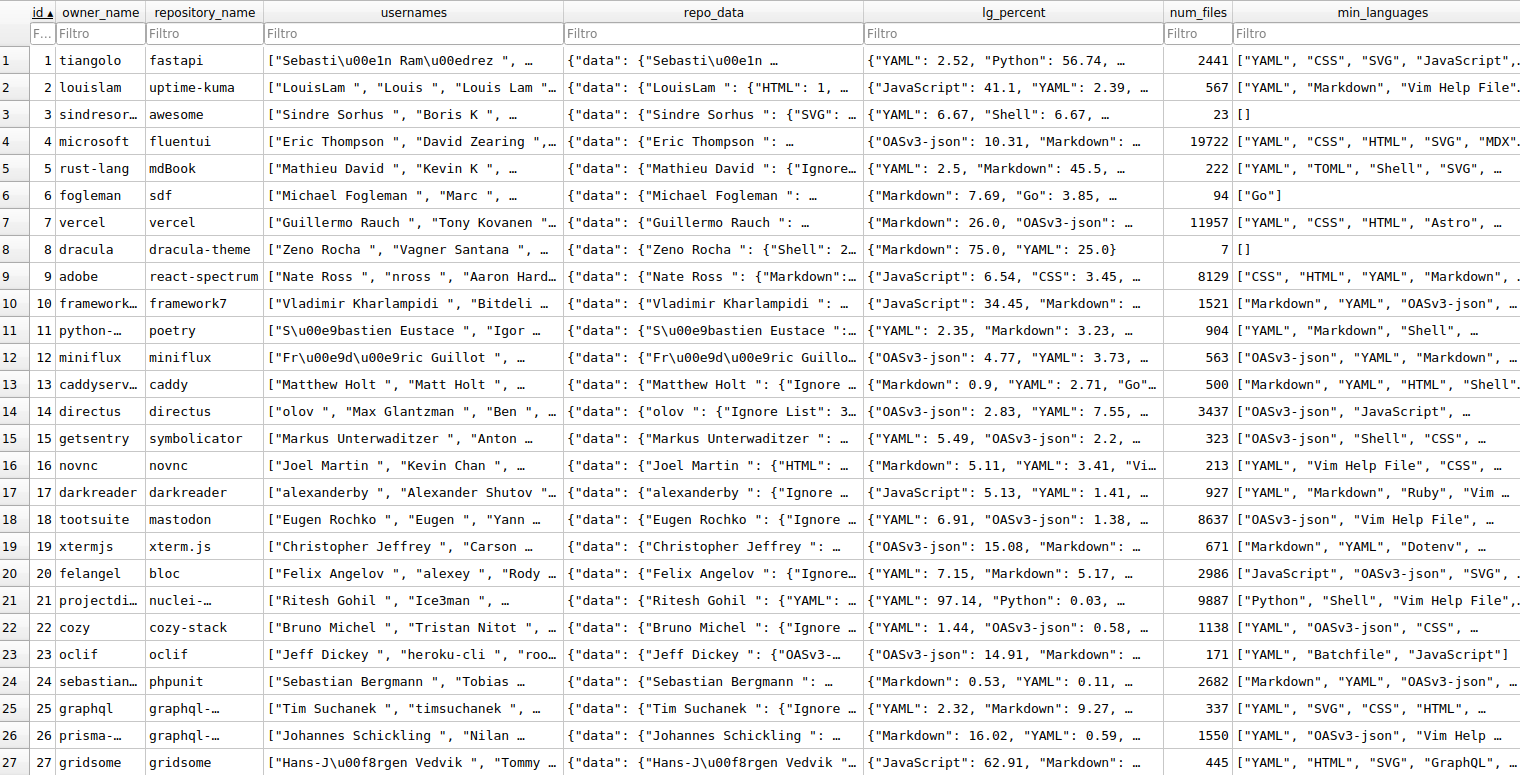
\includegraphics[width=1\textwidth]{img/tablarepo1.png}
  \caption{Estado de la tabla Repository después del análisis de 200 repositorios}
  \label{figura:repoafter1}
\end{figure}

\begin{figure}[H]
  \centering
  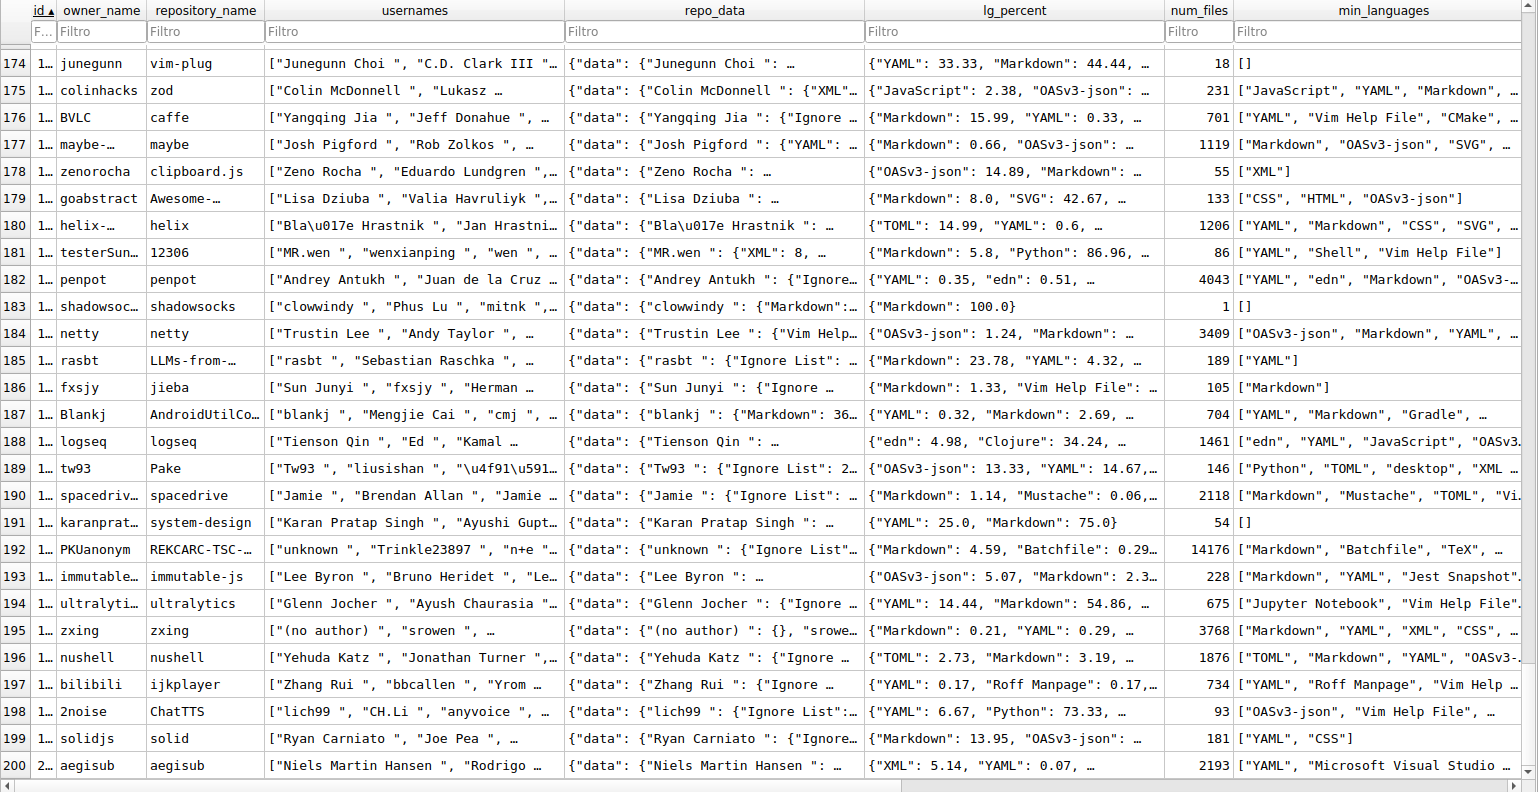
\includegraphics[width=1\textwidth]{img/tablarepo3.png}
  \caption{Estado de la tabla Repository después del análisis de 200 repositorios - 2}
  \label{figura:repoafter2}
\end{figure}

En total, se han registrado en la base de datos 92.816 usuarios que hayan contribuido a alguno o varios de entre los 200 repositorios que se han analizado. Se muestra en las figuras 6.3 y 6.4, con el estado de la tabla User\_expertise. Cada fila presenta un usuario y las columnas los datos que se almacenan de cada uno de ellos.

\begin{figure}[H]
  \centering
  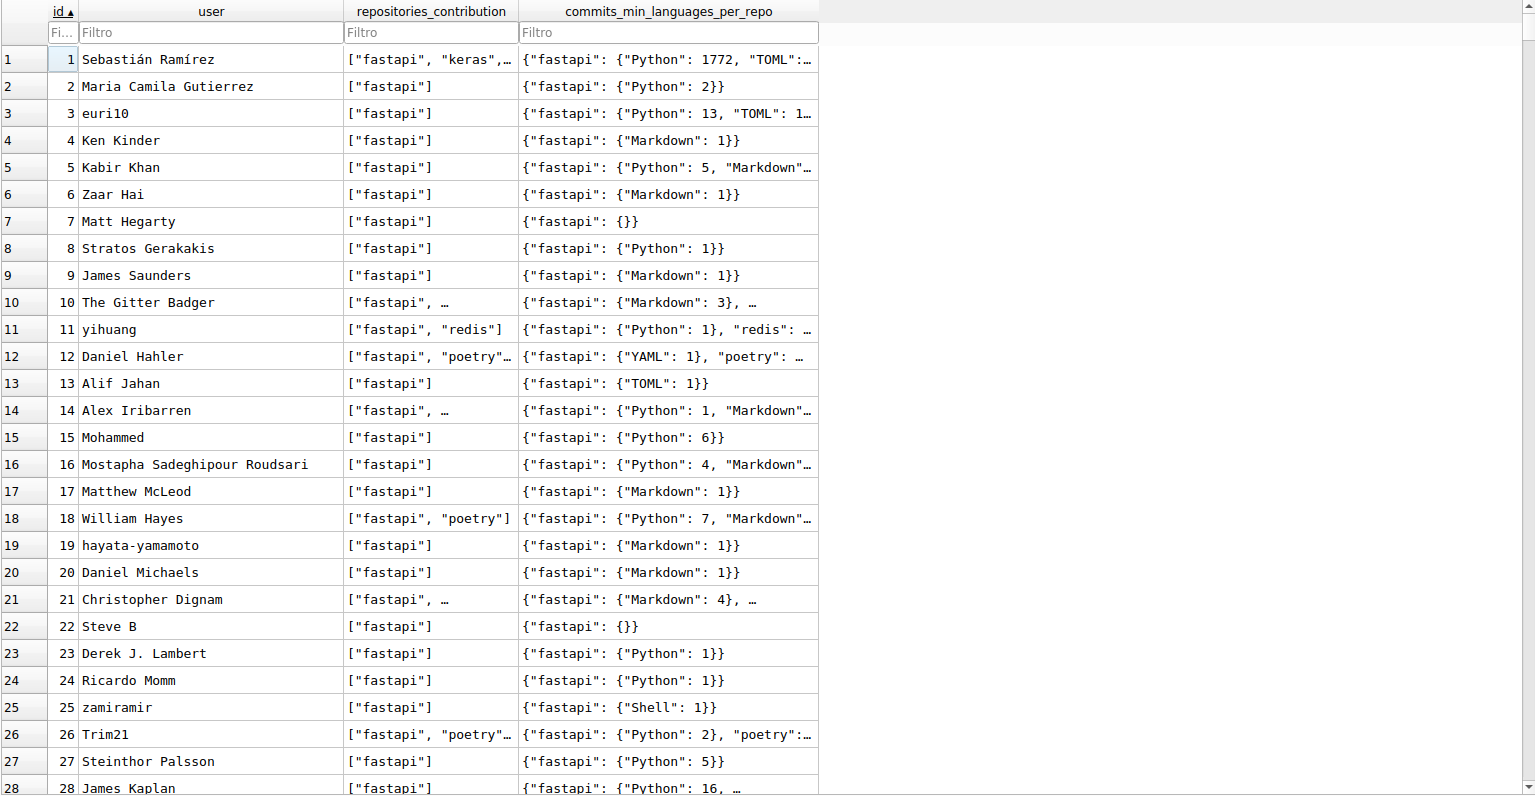
\includegraphics[width=1\textwidth]{img/tablauserexp1.png}
  \caption{Estado de la tabla User\_expertise después del análisis de 200 repositorios}
  \label{figura:userexpafter1}
\end{figure}

\begin{figure}[H]
  \centering
  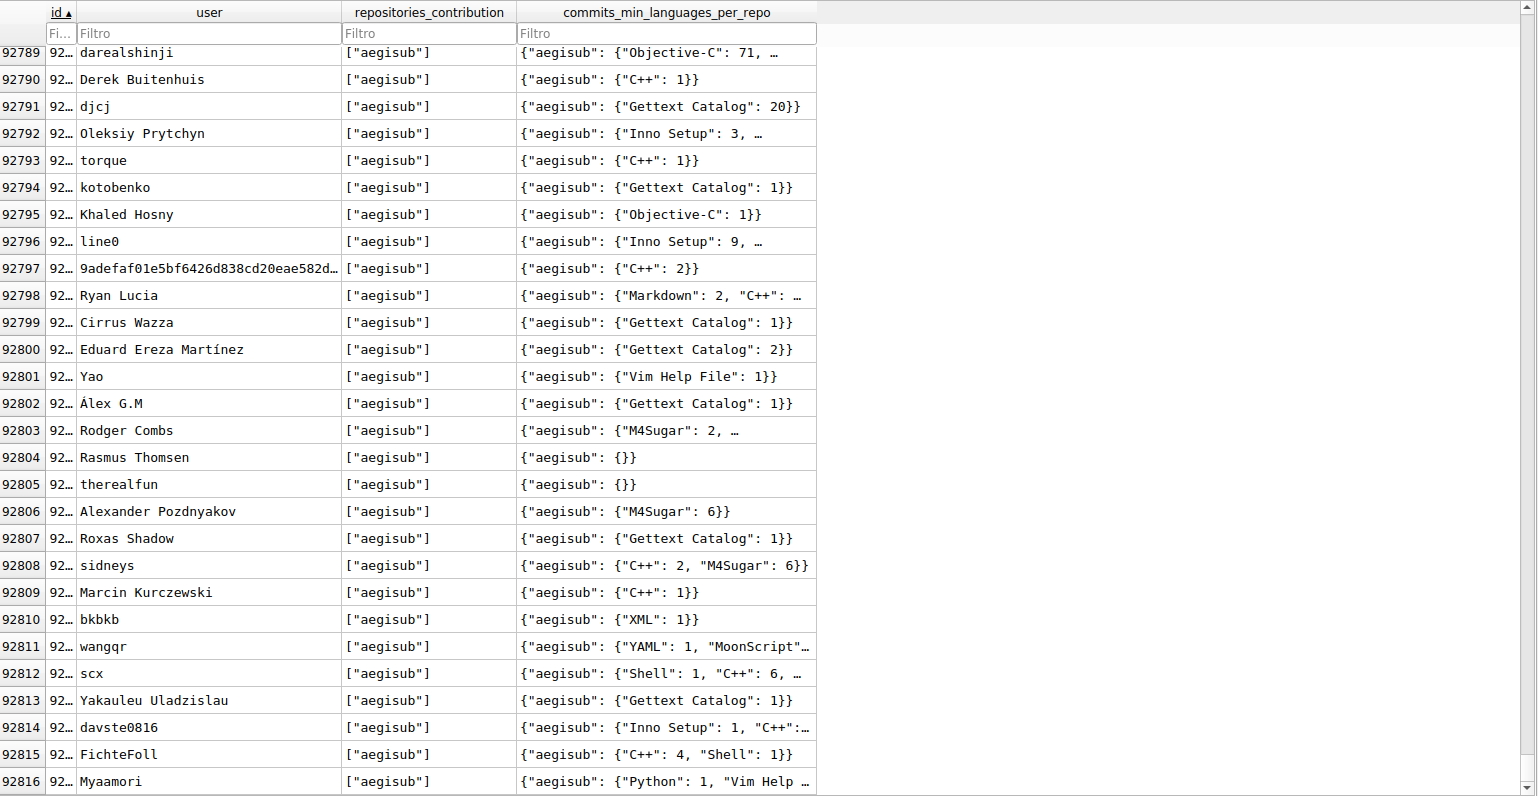
\includegraphics[width=1\textwidth]{img/tablauserexp2.png}
  \caption{Estado de la tabla User\_expertise después del análisis de 200 repositorios - 2}
  \label{figura:userexpafter2}
\end{figure}

En la tabla Languages se han almacenado 262 lenguajes distintos. En las figuras 6.5 y 6.6 se muestra el estado de la tabla Languages tras analizar los 200 repositorios. Cada fila representa un lenguaje y las columnas, los datos que se almacenan de cada lenguaje.

\begin{figure}[H]
  \centering
  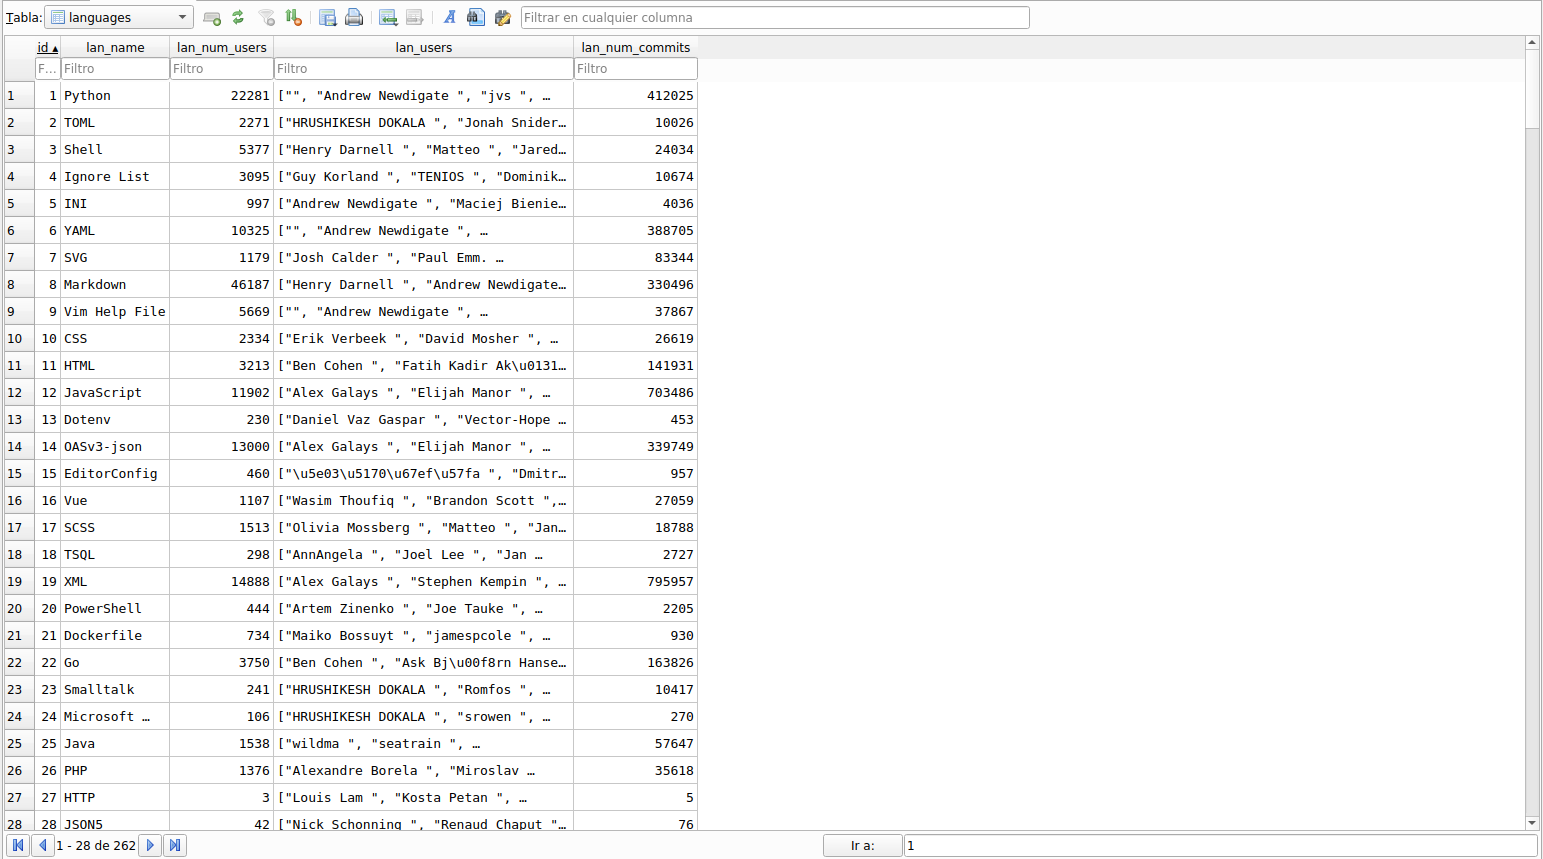
\includegraphics[width=1\textwidth]{img/tablalan1.png}
  \caption{Estado de la tabla Languages después del análisis de 200 repositorios}
  \label{figura:lanafter1}
\end{figure}

\begin{figure}[H]
  \centering
  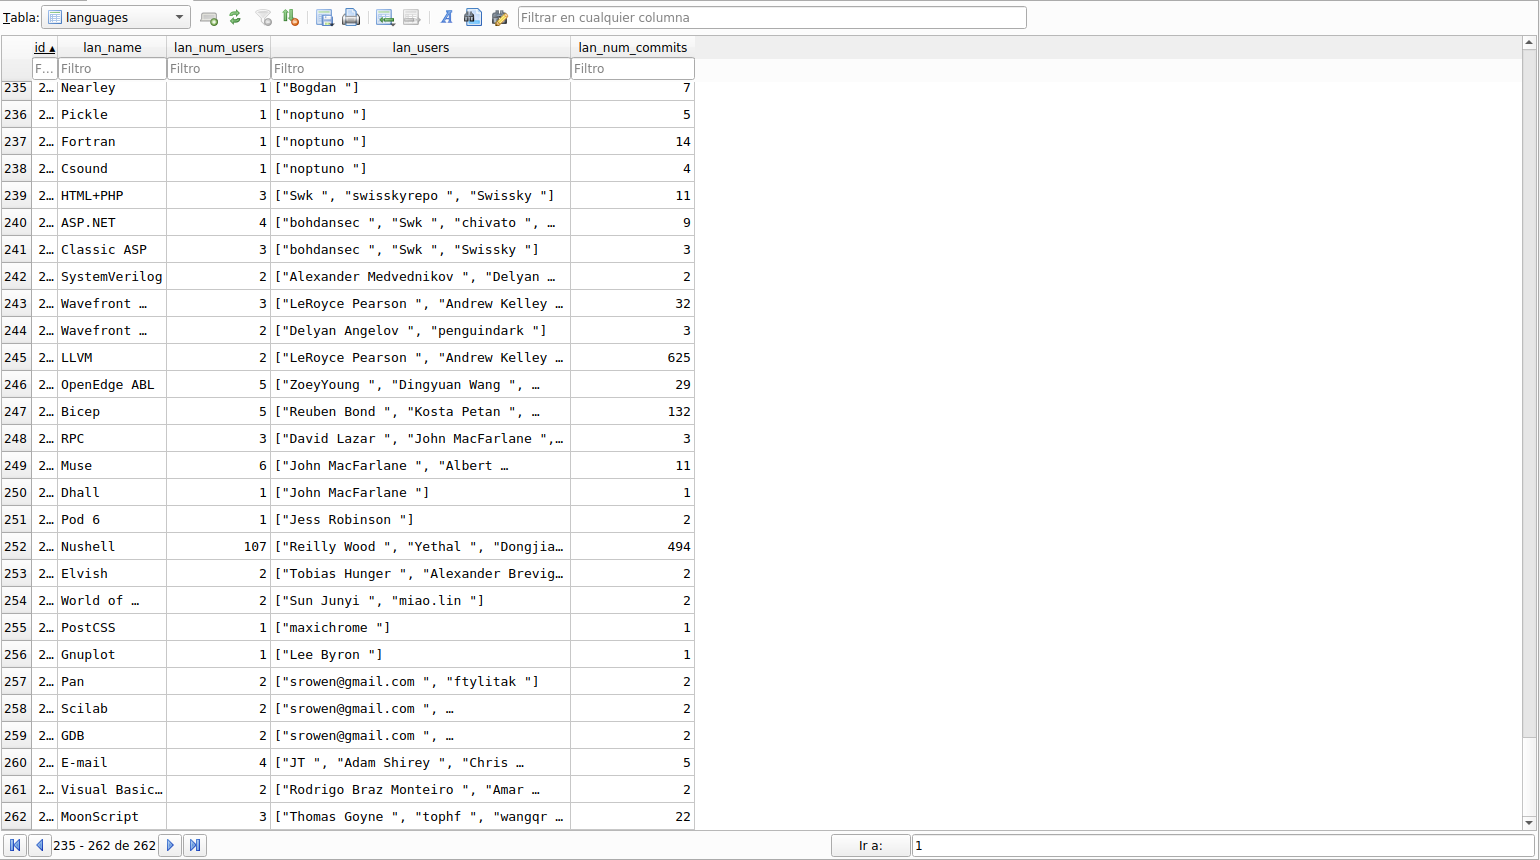
\includegraphics[width=1\textwidth]{img/tablalan2.png}
  \caption{Estado de la tabla Languages después del análisis de 200 repositorios - 2}
  \label{figura:lanafter2}
\end{figure}


Con estos datos, ahora podemos comprobar como es el uso de los lenguajes en los repositorios. Para ello nos haremos las siguientes preguntas:

\begin{itemize}
  \item \textbf{¿Cuáles son los 10 lenguajes sobre los que más usuarios han realizado commits en los distintos repositorios analizados?}
        \begin{itemize}
          \item Viendo la tabla Languages, y ordenando según la columna lan\_num\_users: 
          \begin{itemize}
            \item Markdown: 46187 usuarios
            \item Python: 22281 usuarios
            \item XML: 14888 usuarios
            \item JSON:13000 usuarios
            \item JavaScript: 11092 usuarios
            \item YAML: 10325 usuarios
            \item Vim Help File (TXT): 5669 usuarios
            \item C++: 5587 usuarios
            \item Shell: 5377 usuarios
            \item Go: 3750 usuarios.
          \end{itemize}
        \end{itemize}
  \item \textbf{¿Cuáles son los 10 lenguajes sobre los que se han realizado más commits en total?}
        \begin{itemize}
          \item Viendo la tabla Languages, y ordenando según la columna lan\_num\_commits:
          \begin{itemize}
            \item XML: 795957
            \item JavaScript: 703486
            \item Python: 412025
            \item YAML: 388705
            \item JSON: 339749
            \item Markdown: 330496
            \item Go: 163826
            \item HTML: 141931
            \item C++: 126958
            \item Objective-C: 97321.
          \end{itemize}
        \end{itemize}
  \item \textbf{¿Cuáles son los 10 lenguajes que en más repositorios han sido minoritarios?}
        \begin{itemize}
          \item Haciendo la siguiente query contra la base de datos:
                \begin{verbatim}
      WITH RECURSIVE split_languages AS (
      SELECT 
        id,
        TRIM(REPLACE(REPLACE(SUBSTR(min_languages, 1, 
        INSTR(min_languages || ',', ',') - 1), '[', '')
        , ']', '')) AS language,
        SUBSTR(min_languages, INSTR(min_languages 
        || ',', ',') + 1) AS remaining_languages
        FROM repository
        WHERE min_languages IS NOT NULL
        UNION ALL

        SELECT 
            id,
            TRIM(REPLACE(REPLACE(SUBSTR(remaining_languages
            , 1, INSTR(remaining_languages || ',', ',')
             - 1), '[', ''), ']', '')),
            SUBSTR(remaining_languages, 
            INSTR(remaining_languages || ',', ',') + 1)
        FROM split_languages
        WHERE remaining_languages != ''
        )
        SELECT 
            language, 
            COUNT(*) AS frequency
        FROM split_languages
        WHERE language != ''
        GROUP BY language
        ORDER BY frequency DESC;
      \end{verbatim}
                Obtenemos que los 10 lenguajes que más se han repetido como minoritarios han sido: 
                \begin{itemize}
                  \item YAML: 130 veces
                  \item Vim Help File (TXT): 115 veces
                  \item Shell: 96 veces
                  \item CSS: 92 veces
                  \item SVG: 88 veces
                  \item JSON: 85 veces
                  \item HTML: 85 veces
                  \item Markdown: 70 veces
                  \item Javascript: 63 veces
                  \item TOML: 58 veces.
                \end{itemize}
        \end{itemize}
  \item \textbf{¿Si nos fijamos en los lenguajes minoritarios que más se repiten en los repositorios, cuál es la tendencia de uso por parte de los contribuyentes?}
        \begin{itemize}
          \item Ayudándonos de la tabla Languages, vamos a ver si estos lenguajes se han usado por muchos usuarios, y la cantidad de commits que estos han realizado.
                \begin{itemize}
                  \item YAML: Entre 10325 usuarios se han realizado 388705 commits.
                  \item VIM: Entre 5669 usuarios se han realizado 37867 commits.
                  \item Shell: Entre 5377 usuarios se han realizado 24034 commits.
                  \item CSS: Entre 2334 usuarios se han realizado 26619 commits.
                  \item SVG: Entre 1179 usuarios se han realizado 83344 commits.
                  \item JSON: Entre 13000 usuarios se han realizado 339749 commits.
                  \item HTML: Entre 3213 usuarios se han realizado 141931 commits.
                  \item Markdown: Entre 46187 usuarios se han realizado 330496 commits.
                  \item JavaScript: Entre 11902 usuarios se han realizado 703486 commits.
                  \item TOML: Entre 2271 usuarios se han realizado 10026 commits.
                \end{itemize}
        \end{itemize}
  \item \textbf{¿Cómo es el uso de los lengajes minoritarios dentro de los repositorios? ¿Se centralizan en usuarios concretos? ¿Qué tipo de lenguajes suelen ser?}
        \begin{itemize}
          \item En la mayoría de los repositorios que se han analizado, la tendencia que se sigue es que, si bien no se suelen centralizar del todo en uno o un grupo pequeño de usuarios, si que suele ocurrir que uno o varios de ellos destacan más en el uso de alguno de los lenguajes. Por ejemplo, con el repositorio prettier/prettier que se ha analizado, más de 20 personas han realizado commits sobre ficheros de lenguaje YAML, pero la mayoría de ellos han realizado menos de 3 commits, mientras que la persona con más commits ha realizado 1081 commits, y el segundo, 351 commits. También tiene que ver con el número de commits que se realiza sobre cada uno de los lenguajes, ya que la tendencia que he comentado se suele dar sobre todo para aquellos lenguajes sobre los que se han realizado muchos commits, mientras que para los lenguajes con menos contribuciones, están más repartidos y no hay ningún usuario que destaque demasiado por encima del resto.
          
          Los lenguajes que suelen ser minoritarios en la mayoría de repositorios se utilizan para realizar configuraciones o despliegues de aplicaciones y que suelen ser flexibles de manera que la mayoría de lenguajes de programación pueden usar. Por ello son tan importantes a pesar de que no sean los lenguajes con un mayor uso dentro de los repositorios, ya que suelen ser clave para el funcionamiento de una aplicación, un programa, etc.
        \end{itemize}
  \item \textbf{¿Cómo es el uso general de los lenguajes minoritarios en los repositorios públicos?}
        \begin{itemize}
          \item Para ver el uso general de los lenguajes minoritarios vamos a calcular el coeficiente de Gini de los lenguajes minoritarios más usados en los repositorios que hemos analizado.
          El coeficiente de Gini~\cite{gini:_gini} es una medida de desigualdad que normalmente se suele usar para calcular la desigualdad de ingresos o de población. Sin embargo, se puede usar para medir cualquier distribución desigual. El coeficiente de Gini puede tener un valor entre 0 y 1, siendo 0 la perfecta igualdad, mientras que el 1 es la desigualdad total. Se calcula con la siguiente fórmula matemática:

          \begin{figure}[H]
            \centering
            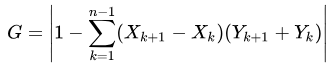
\includegraphics[width=0.6\textwidth]{img/giniformula.png}
            \caption{Fórmula de Brown usada para el cálculo del coeficiente de Gini}
            \label{figura:giniformula}
          \end{figure}
          
          donde:
            \begin{itemize}
              \item G es el Coeficiente de Gini
              \item X suele ser la proporción de población
              \item Y suele ser la proporción de ingresos.
            \end{itemize}
          Y se suele representar de la siguiente manera, con la línea de máxima igualdad, y la curva de Lorenz:
            
          \begin{figure}[H]
            \centering
            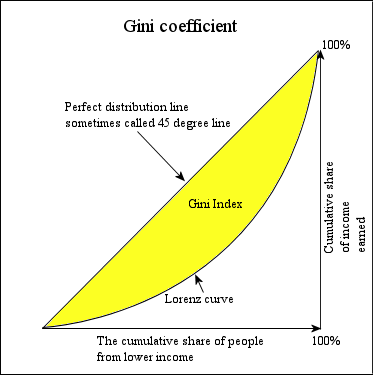
\includegraphics[width=0.6\textwidth]{img/graficagini.png}
            \caption{Gráfica Coeficiente de Gini}
            \label{figura:ginigrafica}
          \end{figure}

          En nuestro caso, al analizar la participación en los lenguajes teniendo en cuenta el número de contribuyentes y el número de commits, cambiaremos la proporción de población e ingresos por nuestros datos. Por tanto, si el coeficiente de Gini que obtenemos del uso de un lenguaje es cercano o igual a 0, significa que el uso es muy parecido entre los contribuyentes, mientras que si se acerca al 1 quiere decir que hay usuarios que contribuyen en mucha mayor cantidad que otros.W

          Con ello, los datos que hemos obtenido en los 10 lenguajes minoritarios que más se repiten son:

          \textbf{YAML: Coeficiente de Gini 0,739}

          \begin{figure}[H]
            \centering
            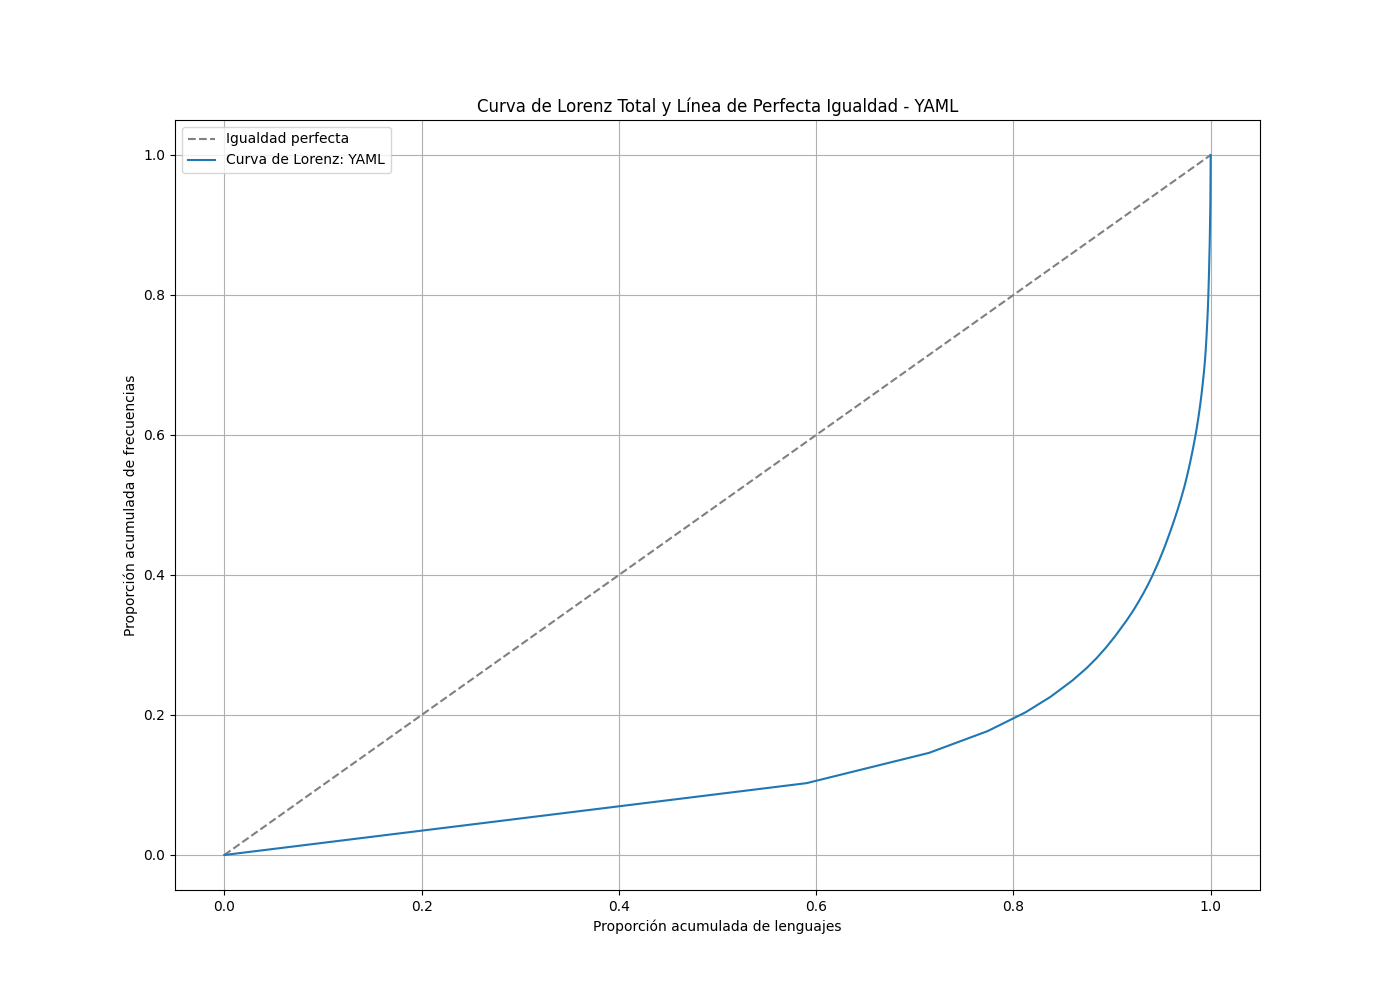
\includegraphics[width=0.8\textwidth]{img/curva_lorenz_total_YAML.png}
            \caption{Coeficiente de Gini YAML}
            \label{figura:ginigraficaYAML}
          \end{figure}

          \textbf{VIM Help File: Coeficiente de Gini 0,750}

          \begin{figure}[H]
            \centering
            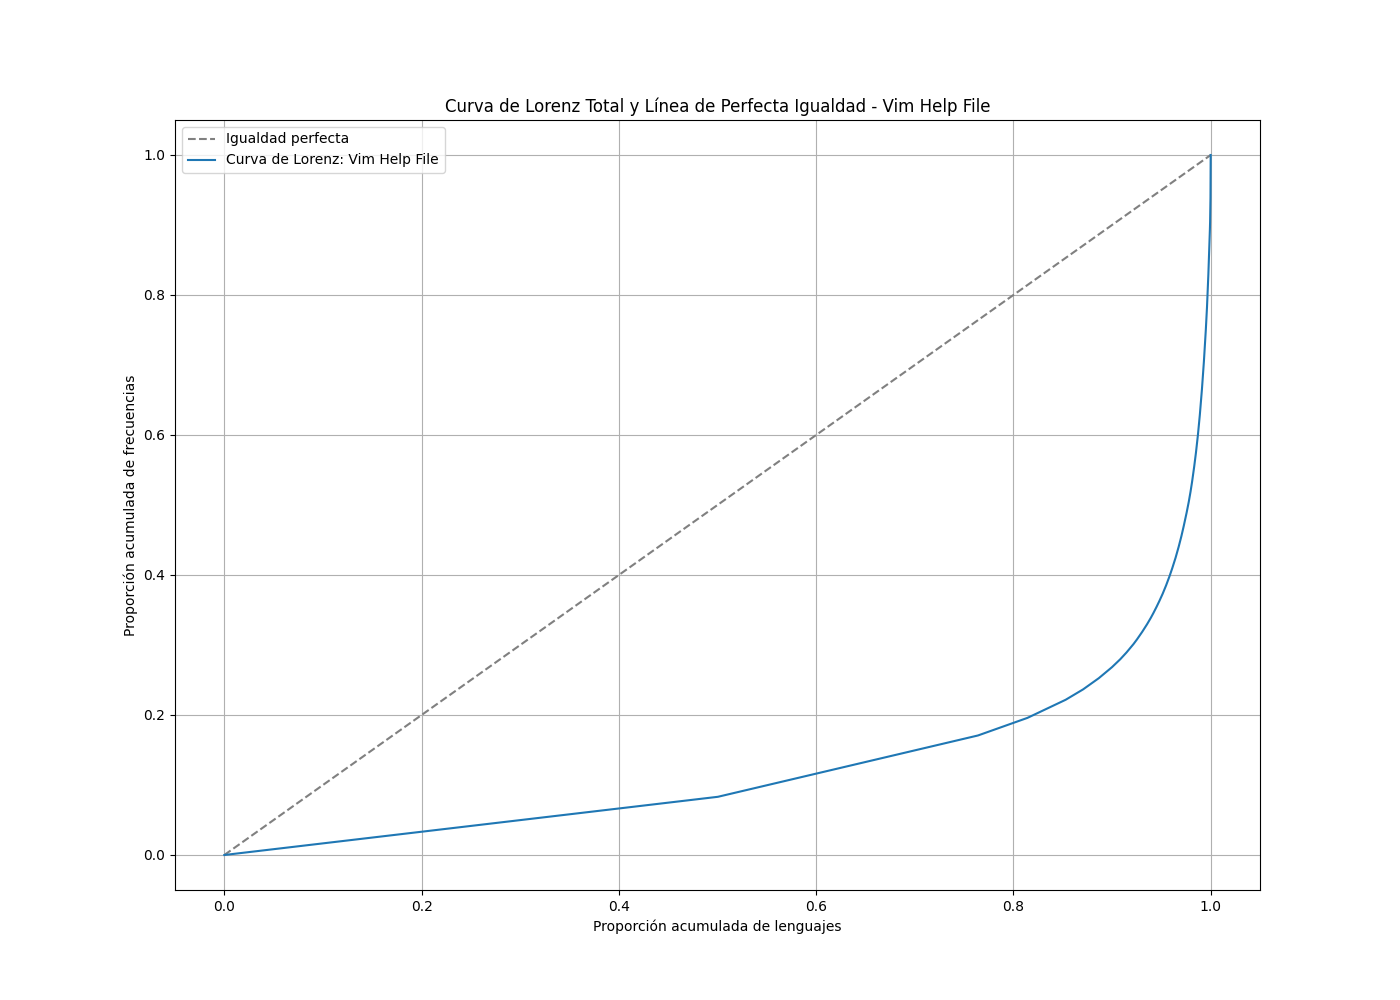
\includegraphics[width=0.8\textwidth]{img/curva_lorenz_total_Vim Help File.png}
            \caption{Coeficiente de Gini VIM Help File}
            \label{figura:ginigraficaVIM}
          \end{figure}

          \textbf{Shell: Coeficiente de Gini 0,699}

          \begin{figure}[H]
            \centering
            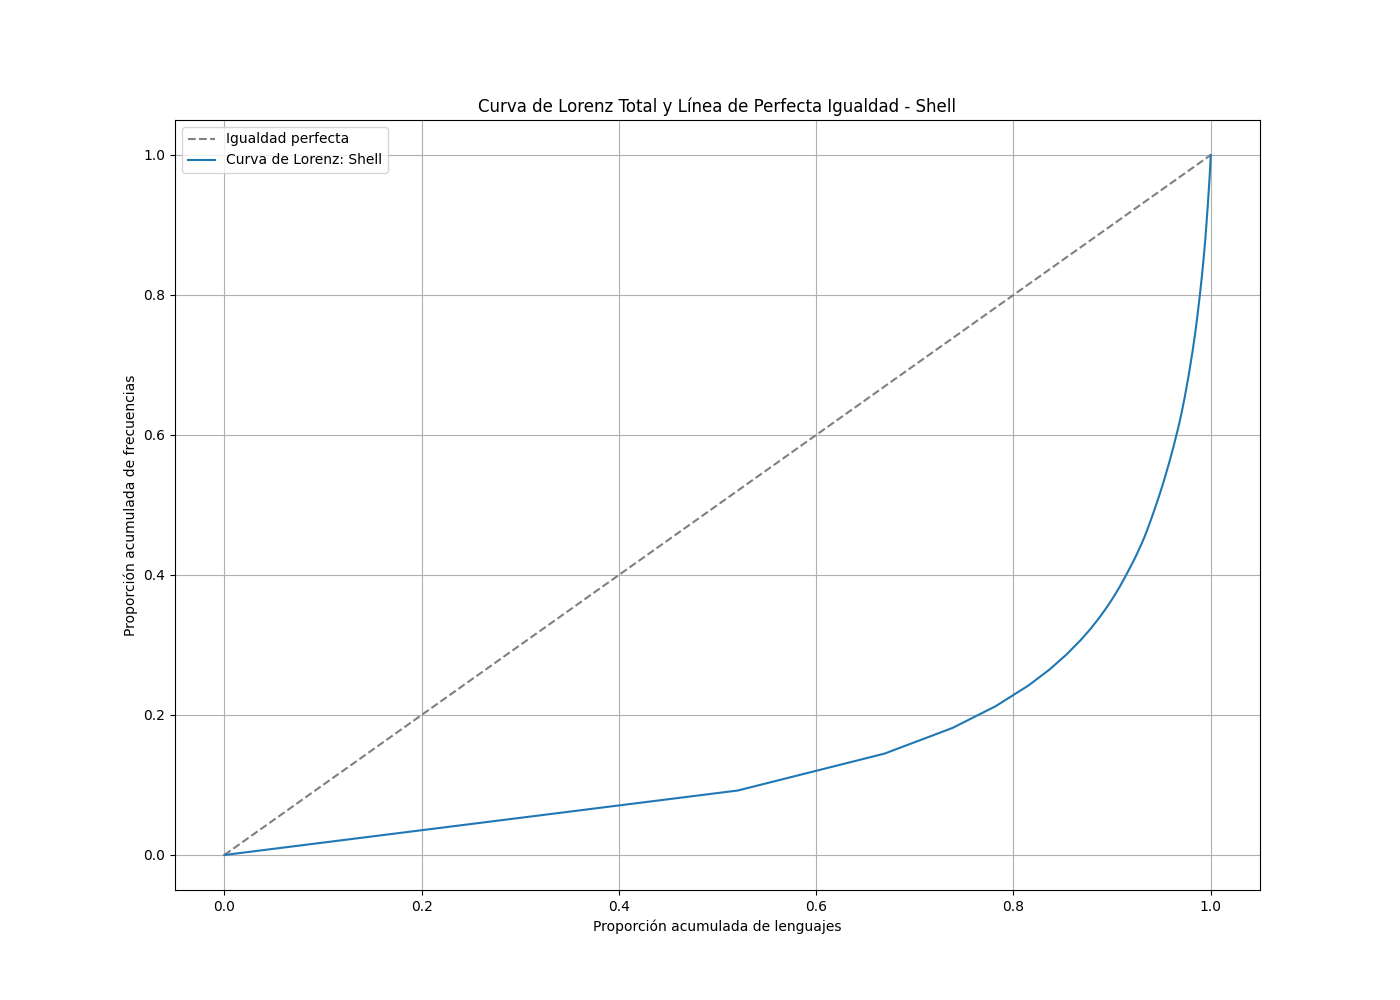
\includegraphics[width=0.8\textwidth]{img/curva_lorenz_total_Shell.png}
            \caption{Coeficiente de Gini Shell}
            \label{figura:ginigraficaShell}
          \end{figure}

          \textbf{CSS: Coeficiente de Gini 0,814}

          \begin{figure}[H]
            \centering
            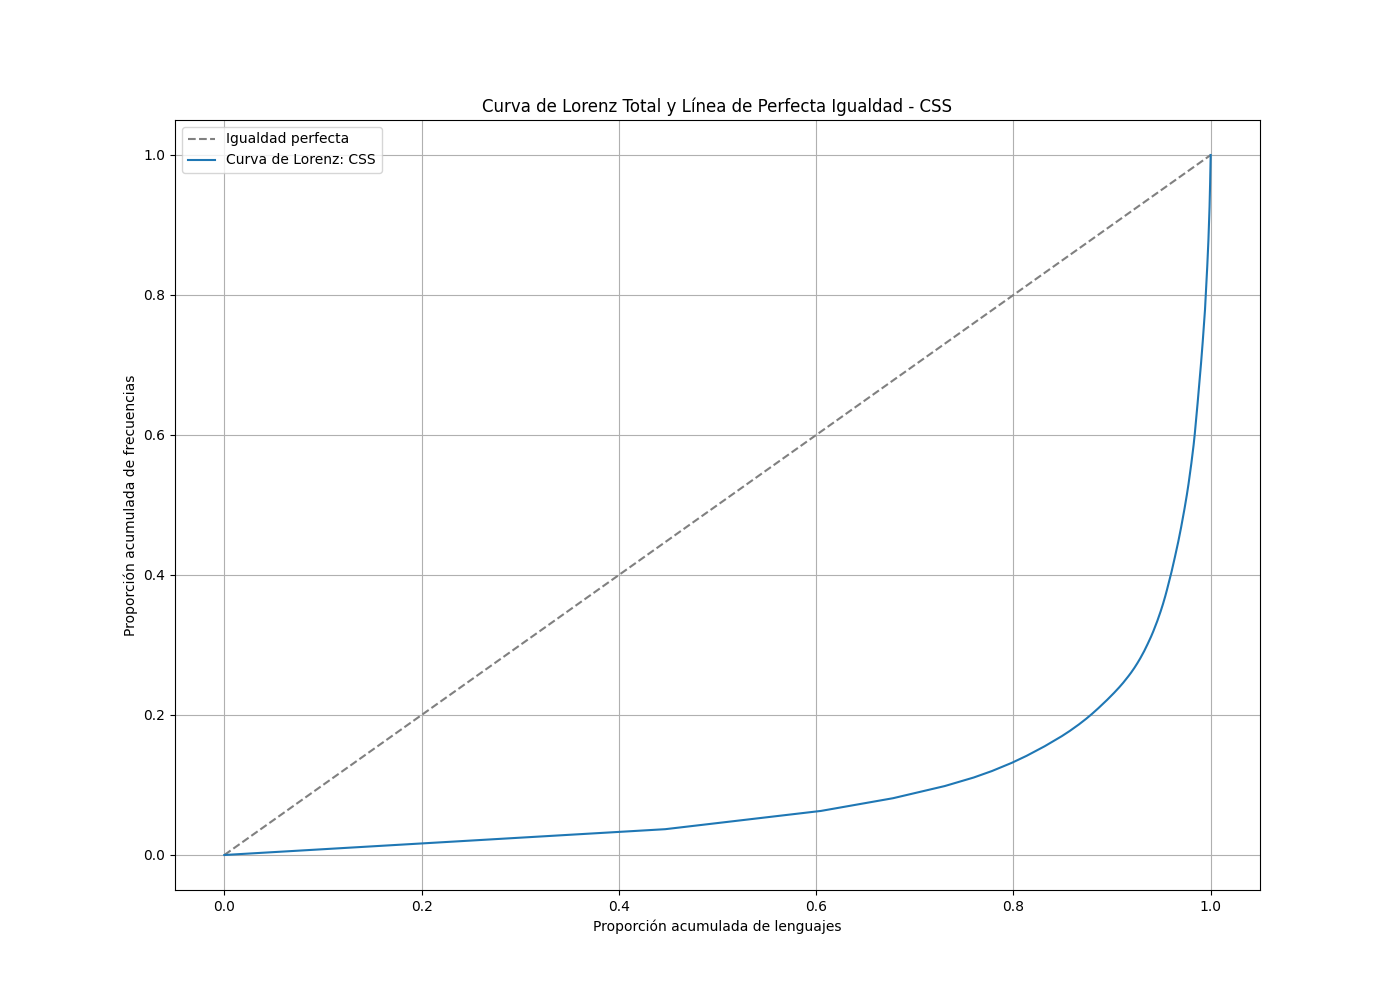
\includegraphics[width=0.8\textwidth]{img/curva_lorenz_total_CSS.png}
            \caption{Coeficiente de Gini CSS}
            \label{figura:ginigraficaCSS}
          \end{figure}

          \textbf{SVG: Coeficiente de Gini 0,814}

          \begin{figure}[H]
            \centering
            \includegraphics[width=0.8\textwidth]{img/curva_lorenz_total_SVG.png}
            \caption{Coeficiente de Gini SVG}
            \label{figura:ginigraficaSVG}
          \end{figure}

          \textbf{JSON: Coeficiente de Gini 0,879}

          \begin{figure}[H]
            \centering
            \includegraphics[width=0.8\textwidth]{img/curva_lorenz_total_JSON.png}
            \caption{Coeficiente de Gini JSON}
            \label{figura:ginigraficaJSON}
          \end{figure}

          \textbf{HTML: Coeficiente de Gini 0,960}

          \begin{figure}[H]
            \centering
            \includegraphics[width=0.8\textwidth]{img/curva_lorenz_total_HTML.png}
            \caption{Coeficiente de Gini HTML}
            \label{figura:ginigraficaHTML}
          \end{figure}

          \textbf{Markdown: Coeficiente de Gini 0,828}

          \begin{figure}[H]
            \centering
            \includegraphics[width=0.8\textwidth]{img/curva_lorenz_total_Markdown.png}
            \caption{Coeficiente de Gini Markdown}
            \label{figura:ginigraficaMarkdown}
          \end{figure}

          \textbf{JavaScript: Coeficiente de Gini 0,896}
          
          \begin{figure}[H]
            \centering
            \includegraphics[width=0.8\textwidth]{img/curva_lorenz_total_JavaScript.png}
            \caption{Coeficiente de Gini JavaScript}
            \label{figura:ginigraficaJavaScript}
          \end{figure}

          \textbf{TOML: Coeficiente de Gini 0,674}

          \begin{figure}[H]
            \centering
            \includegraphics[width=0.8\textwidth]{img/curva_lorenz_total_TOML.png}
            \caption{Coeficiente de Gini TOML}
            \label{figura:ginigraficaTOML}
          \end{figure}




          Con esto se comprueba que la mayoría de lenguajes minoritarios de los repositorios que hemos analizado tienen un uso bastante desigual ya que todos se acercan bastante al 1. Esto quiere decir que en estos lenguajes suelen aportar bastante más unos pocos usuarios que el resto que contribuyen a estos. 

    \end{itemize}
  \end{itemize}
        %%%%%%%%%%%%%%%%%%%%%%%%%%%%%%%%%%%%%%%%%%%%%%%%%%%%%%%%%%%%%%%%%%%%%%%%%%%%%%%%
        %%%%%%%%%%%%%%%%%%%%%%%%%%%%%%%%%%%%%%%%%%%%%%%%%%%%%%%%%%%%%%%%%%%%%%%%%%%%%%%%
        % CONCLUSIONES %
        %%%%%%%%%%%%%%%%%%%%%%%%%%%%%%%%%%%%%%%%%%%%%%%%%%%%%%%%%%%%%%%%%%%%%%%%%%%%%%%%

        \cleardoublepage
        \chapter{Conclusiones}
        \label{chap:conclusiones}


        \section{Consecución de objetivos}
        \label{sec:consecucion-objetivos}

        El objetivo general se ha conseguido a base de la cumplimentación de los objetivos específicos que se pusieron al comenzar el proyecto.

        \begin {itemize}
  \item \textbf {Obtención de datos de los repositorios de plataformas Git}: Este objetivo se ha logrado cumplir gracias, sobre todo, al uso de la librería Perceval, que ha permitido la recolección de los datos de los commits de los distintos repositorios y en la cual se basa la aplicación para hacer los análisis. Además, también, mediante llamadas a la API de GitHub se obtienen datos adicionales sobre los repositorios como el número de ficheros del repositorio o los lenguajes usados en él.
  \item \textbf{Tratamiento de los datos de los repositorios}: Los datos que recolectamos tanto con Perceval como con nuestras propias llamadas a la API de Github se reciben en formato JSON. La aplicación adapta las respuestas a los  formatos que necesitamos para realizar los análisis y guardarlos en la base de datos según estaba definido.
  \item \textbf{Creación de una aplicación web para permitir un uso más fácil del aplicativo}: Mediante el uso del módulo de Flask de Python, se ha podido crear la aplicación web, formada sobre todo con HTML, CSS, JavaScript y usando la librería Bootstrap. Se ha conseguido que la experiencia del usuario que entra a la web sea más sencilla para el uso de la aplicación y que pueda ver gráficamente los análisis de los repositorios que escoja.
  \item \textbf{Creación de una base de datos donde almacenar los análisis de los repositorios}: Se ha conseguido complir este objetivo gracias a la base de datos SQLite3 que se ha creado. Además, logramos almacenar todos los datos que buscábamos para realizar los análisis finales. Quizá este sea el punto que, si bien se ha conseguido, se podría mejorar ya que la clasificación de las diferentes tablas y sus propias columnas que se ha hecho durante el proyecto, es mejorable de cara a poder sacar los datos y poder analizarlos de una manera más fácil a posteriori.
\end{itemize}

Debido a la consecución de todos estos objetivos, damos por cumplido el objetivo general del proyecto mediante nuestro programa en Python que procesa los datos obtenidos de los repositorios y que analiza el proyecto, junto a la aplicación web que permite visualizar fácilmente el análisis realizado.

\section{Aplicación de lo aprendido}
\label{sec:aplicacion}

Para la realización de este trabajo de fin de grado he aplicado conocimientos adquiridos a lo largo de todas la carrera universitaria, sobre todo de aquellas asignaturas dirigidas a la programación.

\begin{enumerate}
  \item \textbf{Informática 1}: Con esta asignatura comencé a conocer los fundamentos de la programación. Si bien el lenguaje que practiqué fue Picky, me ayudó a saber los conceptos más básicos.
  \item \textbf{Informática 2}: En esta asignatura, ya más centrada en programación más avanzada, pude ampliar mi conocimiento del lenguaje Python usado en este proyecto.
  \item \textbf{Protocolos para la Transmisión de Audio y Vídeo}: Fue la primera asignatura en la que comencé a conocer Python y a aplicarlo. Probablemente, sea la que más me ha ayudado con este proyecto, ya que también hice una aplicación cliente-servidor, por lo que ya algo de experiencia.
  \item \textbf{Construcción de Servicios y Aplicaciones Audiovisuales en Internet}: En esta asignatura comencé a tratar como funciona el front-end de una aplicación web, practicando con HTML, CSS y JavaScript, con lo que se ha construido el cliente de mi web.
  \item \textbf{Laboratorio de Tecnologías Audiovisuales en la web}: En esta asignatura conocí como funciona el back-end de una plataforma web, con lo que a la hora de hacer el servidor, pude aplicar algunos de los conceptos que aprendí.
\end{enumerate}


\section{Lecciones aprendidas}
\label{sec:lecciones_aprendidas}

Durante la realización de este trabajo de fin de grado he aprendido:

\begin{enumerate}
  \item Uso de la librería Perceval para la obtención de datos de repositorios Git.
  \item Uso de la librería Flask apra la creación de la aplicación web.
  \item Uso de distintas librerías como matplotlib para la representación del análisis de los repositorios
  \item Creación de una base de datos SQLite3.
  \item Manejo de una base de datos y la interacción con la aplicación Python.
  \item El uso de distintos lenguajes en repositorios de GitHub.
  \item Organización de proyectos en cuanto a tiempo y esfuerzo.
\end{enumerate}


\section{Trabajos futuros}
\label{sec:trabajos_futuros}

Tras finalizar el proyecto y hacer un análisis general de lo que se puede mejorar, cambiar o añadir a la aplicación, tengo las siguientes propuestas a futuro:

\begin{itemize}
\item \textbf{Mejorar la clasificación de la base de datos}: Como he comentado en un punto anterior, este es el principal punto de mejora que le encuentro a la aplicación. Me ha sido bastante complicado hacer el análisis final del uso de los lenguajes minoritarios en los repositorios debido a como he almacenado los datos en la tabla Repository. Creo que sería mejor almacenar los datos en más columnas, y sin usar formatos JSON o listas.
\item \textbf{Añadir en la aplicación páginas que permitan ver los repositorios que ya están en la base de datos}: Creo que sería útil para el usuario que entre a la página, que pueda acceder al análisis de los repositorios sin tener que buscarlos antes, es decir, una página que muestre una tabla con todos los repositorios que están en la base de datos y los pueda ver fácilmente.
\item \textbf{Mejorar los tiempos de recolección de datos}: Perceval quizá es un poco lento a la hora de generar los ficheros JSON con los datos en repositorios que tienen una gran cantidad de commits realizados. Puede que haya una mejor alternativa para mejorar la eficiencia de este punto.
\end{itemize}
%%%%%%%%%%%%%%%%%%%%%%%%%%%%%%%%%%%%%%%%%%%%%%%%%%%%%%%%%%%%%%%%%%%%%%%%%%%%%%%%
%%%%%%%%%%%%%%%%%%%%%%%%%%%%%%%%%%%%%%%%%%%%%%%%%%%%%%%%%%%%%%%%%%%%%%%%%%%%%%%%
% APÉNDICE(S) %
%%%%%%%%%%%%%%%%%%%%%%%%%%%%%%%%%%%%%%%%%%%%%%%%%%%%%%%%%%%%%%%%%%%%%%%%%%%%%%%%

\cleardoublepage
\appendix
\chapter{Manual de usuario}
\label{app:manual}

Al entrar en la aplicación se muestra esta pantalla:

\begin{figure}[H]
  \centering
  \includegraphics[width=1\textwidth]{img/paginaprincipal.png}
  \caption{Página inicial de la aplicación}
  \label{figura:appmainpage2}
\end{figure}

  Al clicar en Búsqueda de un repositorio concreto se muestra esta pantalla:

  \begin{figure}[H]
    \centering
    \includegraphics[width=1\textwidth]{img/userrepoget.png}
    \caption{Respuesta con el formulario a la petición con método GET}
    \label{figura:userrepoget2}
  \end{figure}

  Se debe introducir el nombre de usuario de GitHub y el nombre del repositorio a analizar y al enviarlo se muestra la siguiente pantalla:
  \begin{figure}[H]
    \centering
    \includegraphics[width=1\textwidth]{img/httpie.png}
    \caption{Respuesta con el análisis del repositorio}
    \label{figura:httpie}
  \end{figure}

  Al hacer clic sobre los lenguajes o los usuarios aparece la información detallada acerca de ellos.

  Si en la pantalla principal se pulsa en "Búsqueda por usuario" se muestra la siguiente pantalla:

  \begin{figure}[H]
    \centering
    \includegraphics[width=1\textwidth]{img/usersearchget.png}
    \caption{Respuesta a la petición GET al endpoint /usersearch}
    \label{figura:usersearch2}
  \end{figure}

  Se debe introducir el nombre de usuario de GitHub, y se muestra una lista de los repositorios de ese usuario:

  \begin{figure}[H]
    \centering
    \includegraphics[width=1\textwidth]{img/httpiesearch.png}
    \caption{Respuesta con los repositorios del usuario}
    \label{figura:httpiesearch}
  \end{figure}

  Al clicar en cualquier repositorio de la lista se pasa a su análisis.

%%%%%%%%%%%%%%%%%%%%%%%%%%%%%%%%%%%%%%%%%%%%%%%%%%%%%%%%%%%%%%%%%%%%%%%%%%%%%%%%
%%%%%%%%%%%%%%%%%%%%%%%%%%%%%%%%%%%%%%%%%%%%%%%%%%%%%%%%%%%%%%%%%%%%%%%%%%%%%%%%
% BIBLIOGRAFIA %
%%%%%%%%%%%%%%%%%%%%%%%%%%%%%%%%%%%%%%%%%%%%%%%%%%%%%%%%%%%%%%%%%%%%%%%%%%%%%%%%

\cleardoublepage

% Las siguientes dos instrucciones es todo lo que necesitas
% para incluir las citas en la memoria
\bibliographystyle{abbrv}
\bibliography{memoria}  % memoria.bib es el nombre del fichero que contiene
% las referencias bibliográficas. Abre ese fichero y mira el formato que tiene,
% que se conoce como BibTeX. Hay muchos sitios que exportan referencias en
% formato BibTeX. Prueba a buscar en http://scholar.google.com por referencias
% y verás que lo puedes hacer de manera sencilla.
% Más información: 
% http://texblog.org/2014/04/22/using-google-scholar-to-download-bibtex-citations/

\end{document}
